%ctrl+alt+b -> build, ctrl+alt+v => preview at new tab
%ctrl+click -> highlight line

% \documentclass[12pt,a4paper,titlepage]{jsarticle}
\documentclass[11pt,a4paper]{jsreport}

\usepackage{algorithmic}
\usepackage{amsmath,amssymb,amsfonts,amsthm,,mathtools}
\usepackage{ascmac}
% \usepackage{amsmath}
\usepackage{bm}
\usepackage{caption}
\usepackage{cite}
\usepackage{comment}
% \usepackage[dvipdfmx]{color}
\usepackage{colortbl}
\usepackage{float}
\usepackage{graphicx}
% \usepackage[dvipdfmx]{graphicx}
\usepackage{multicol}
\usepackage{latexsym}
% \usepackage{listings}
\usepackage[dvipdfmx]{pict2e}
\usepackage[ipaex]{pxchfon}
\usepackage{tabularx}
\usepackage{textcomp}
\usepackage{underscore}
\usepackage{ulem}
\usepackage{url}
\usepackage{wrapfig}
\usepackage[dvipsnames,dvipdfmx]{xcolor}
\usepackage{mdframed}
\usepackage{makecell}
\usepackage{SekineLabMacro}
%\usepackage{physics2}
% \usepackage{amsmath,amssymb}% 数式入力に数学必携のパッケージ読み込み
\usepackage{listings,jvlisting}
% \usepackage{here}
\lstset{
  basicstyle={\ttfamily},
  identifierstyle={\small},
  commentstyle={\smallitshape},
  keywordstyle={\small\bfseries},
  ndkeywordstyle={\small},
  stringstyle={\small\ttfamily},
  frame={tb},
  breaklines=true,
  columns=[l]{fullflexible},
  numbers=left,
  xrightmargin=0zw,
  xleftmargin=3zw,
  numberstyle={\scriptsize},
  stepnumber=1,
  numbersep=1zw,
  lineskip=-0.5ex
}
%プログラムのソースコード関連はここまで

%\setcounter{secnumdepth}{4}
%\usepackage[margin=10truemm]{geometry}

\captionsetup[figure]{labelsep=space}
\captionsetup[table]{labelsep=space}

\theoremstyle{definition}
\newtheorem{dfn}{定義}
\newtheorem{thm}{定理}
\newtheorem{lmm}{補題}

\renewcommand{\qedsymbol}{$\blacksquare$}
\renewcommand{\proofname}{\textbf{証明}}

%============

%\newtheo

%============



\title{AVX-512を用いた区間行列積の実装法}
\author{筒田 峰輔}
\date{12月25日}

\begin{document}

\JYear{令和6年度}
\Kinds{卒業論文}
\StudentNumber{2131104}


\pagestyle{empty}
\maketitle
\tableofcontents
\clearpage
\pagestyle{plain}

\chapter{はじめに}
	ロボットや自動車の動きのシミュレーションなど幅広い分野で利用される数学問題をコンピュータを用いて近似的に解くことを数値計算という. コンピュータは人間より素早く大量に計算を行うことができるが, 正確に計算することが難しい. それはコンピュータが無限桁を表せないという性質を持ち, 数値計算を行った際に途中で桁が切り捨てられ, 誤差が発生する.数値計算では, このような誤差を含んだ計算が繰り返し行われることで無視できない真の解とのズレが発生することがある. そのため,数値計算で得られた近似買いがどれだけの誤差を含んでいるのかを可視化する精度保証が必要になってくる.
	数値計算の中には区間積和演算と呼ばれる
	\begin{equation*}
	a \times b + c
	\end{equation*}
で表される計算がある. 行列積同士の計算にはこの積和演算が用いられる. 実数を用いた演算は, コンピュータ上では浮動小数点として近似して計算され, この時に発生する誤差を丸め誤差という. 計算1回あたりに発生する誤差は僅かだったとしても, 実際には膨大な回数の計算が行われるため, 誤差の範囲がどんどん増えていくことで無視できない誤差になってしまう. これに対し,真の解をもつ区間をある種の数とみなして浮動小数点数によって実数を挟み込み, 区間の幅によって誤差の評価を行う. 区間演算では上端と下端の2つの浮動小数点によって誤差の評価を行う. 例として以下のような区間を持つ行列同士の演算も区間演算によって行われる.

\begin{itembox}[l]{区間行列同士の掛け算}
\[
\begin{pmatrix}
   [a_{11l},a_{11u}] & \cdots & [a_{1nl},a_{1nu}] \\
   \vdots & \ddots & \vdots \\
   [a_{n1l},a_{n1u}] & \cdots & [a_{nnl},a_{nnu}]
 \end{pmatrix}
 \times
 \begin{pmatrix}
   [b_{11l},b_{11u}] & \cdots & [b_{1nl},b_{1nu}] \\
    \vdots & \ddots & \vdots \\
   [b_{n1l},b_{n1u}] & \cdots & [b_{nnl},b_{nnu}]
 \end{pmatrix}
 \]
\end{itembox}

区間行列積の演算では1つの要素を導くためにも以下のような
\begin{equation*}
[a_l,a_u] \cdot [b_l,b_u] + [c_l,c_u]
\end{equation*}
式のように区間を持つ要素同士の積和演算である区間積和演算と呼ばれる計算を複数回行う必要がある. しかし区間積和演算は丸めモードの変更を必要とし,正しく計算するためには最適化の抑制を行う必要があるため, 非常に遅い計算になる. そのため現在では区間行列積の精度保証には精度を犠牲にした中心半径型の区間演算に基づくBLASによる計算で行うことが主である. BLASを用いることで高速な区間行列積の実装を行うことができる. しかし,BLASは点行列を扱う線形代数のサブプログラムであるため, 区間行列をそのまま実装することはできない. そこでBLASでは区間の幅を過大評価することで精度を低下させる代わりに点行列の演算に帰着している[2]. \\
\indent 本論文ではAVX-512を用いることで上端下端型の区間積和演算を高速に計算し, 精度よく高速な区間行列積の実装を目的とする. \\
\indent 本論文の構成を以下に示す. 第2章では基本事項の解説を行う. 第3章では既存手法について示し, 第4章では提案手法について述べる. 第5章では実験とその結果についてまとめ第6章にて結論をまとめる.
\newpage
\chapter{準備}
\section{浮動小数点[1]}
  計算機では実数を扱うとき, 正確に表せないときがある. たとえば,$\sqrt{2}$の値を小数の形で厳密に表
現するには無限の桁が必要であるが, 計算機では, 有限の情報しか扱えない. すなわち, 計算機
では, 有限桁の, そして有限個の数しか扱えないのである.コンピュータでは,実数を近似的に表現する仕組みとして,浮動小数点数(floating point 
number)を採用している. これは, 4つの正の整数$β,n,L,U$で特徴づけられる数であり,
  \begin{equation}
    x = \pm\underbrace{\left( \frac{d_0}{\beta}+\frac{d_1}{\beta_1}+, \cdots ,+\frac{d_n}{\beta_n}\right)}_{=\alpha}\cdot\beta^m
  \end{equation}

\noindent の形をしている. ここで$d_0,...,d_n$と$m$は

  \begin{equation}
    0 \leq d_i \leq \beta - 1(i = 0,1,...,n)d_0 \neq 0, -L \leq m \leq U
  \end{equation}

\noindent を満たす整数とする.$\beta$を基数,$n$を桁数, $L$を最小指数, $U$を最大指数, $\alpha$を$x$の仮数部または
小数部, $m$を指数部という. なお$\beta$は偶数とする. \\
 そして集合

  \begin{equation*}
    \mathbb{F}_s = \mathbb{F}_s(\beta,n,L,U) = \{0\} \cup \{(2.1)と(2.2)で表現される数\}
  \end{equation*}

\noindent を$\beta$進$n + 1$桁の浮動小数点数系と呼ぶ. $\mathbb{F}$の中で, 絶対値最大の正数は$x_{max} = \beta^U(\beta - \beta^{-n})$
であり,絶対値最小の正数は$x_{min} = \beta^{-L}$となる. \\
  計算のため入力した数値や, 計算の途中で算出される中間的な数値, そして最終目標の答えを表
す数値は, すべてそれらに近い$\mathbb{F}_s$の要素で近似的に表現され,使用される. 例えば,$\tilde{x} \in \mathbb{R}$が 

  \begin{equation}
    \tilde{x} = \delta \cdot \left(\frac{d_0}{\beta_0}+, \cdots +\frac{d_n}{\beta_n}+\frac{d_{n+1}}{\beta_{n+1}}+ \cdots \right) \cdot \beta^m
  \end{equation}

\noindent の形で与えられているとする. $\delta$は$+1$か$-1$のいずれかであり, $-L \leq m \leq U$が成り立っている
とする. このとき, $\tilde{x}$の近似値として,

  \begin{equation}
    x = \delta \cdot \left(\frac{d_0}{\beta_0}+, \cdots +\frac{d_n}{\beta_n}\right)\cdot\beta^m
  \end{equation}

\noindent を採用する方法を切り捨てという. また,

  \begin{align}
    & x = \delta\cdot\left(\frac{d_0}{\beta_0}+, \cdots +\frac{\tilde{d}_n}{\beta_n}\right)\cdot\beta^m, \nonumber \\
    \tilde{d_n} &= 
      \begin{cases}
        d_n(d_{n+1} < \beta/\text{2のとき}) \\
        d_n\text{または}d_n+1(d_{n+1} = \beta/2,d_{n+2} = d_{n+3} = \cdots = \text{$0$のとき}) \\
        d_n+1(d_{n+1} = \beta/2,d_{n+2} = d_{n+3} = \cdots = 0\text{の場合を除き}d_{n+1} \geq \beta/\text{2のとき})
      \end{cases}
  \end{align}

\noindent を採用する方法を最近点への丸めという. この方法では,$\tilde{x}$の近似値として, $|x - \tilde{x}|$の値が最小
となるような$x$, すなわち,$|x - \tilde{x}| = min|y - \tilde{x}|$を満たす$x \in \mathbb{F}_s$を採用する. 最近点への丸め
の中でも, $\tilde{x}$が,$x_1$と$x_2$の中点の場合, すなわち,$d_{n+1} = \beta/2,d_{n+2} = d_{n+3} = \cdots = 0$の場合は,

  \begin{equation}
    x_1 = \delta \cdot \left(\frac{d_0}{\beta_0}+, \cdots +\frac{d_n}{\beta_n}\right)\cdot\beta^m,x_2 = \delta \cdot \left(\frac{d_0}{\beta_0}+, \cdots +\frac{d_n+1}{\beta_n}\right)\cdot\beta^m
  \end{equation}

\noindent が$|x_1 - \tilde{x}| = |x_2 - \tilde{x}|$を満たすので, これら2つが$x$の候補となる得る. そのとき,$d_n$の値を考慮して,

  \begin{equation*}
    x = \left\{
    \begin{aligned}
      x_1(d_n\text{が偶数のとき}) \\
      x_2(d_n\text{が奇数のとき})
    \end{aligned}
    \right.
  \end{equation*}

\noindent とする. この方法を最近偶数への丸めという. \\
\indent このように$\tilde{x} \in \mathbb{R}$に$\tilde{x} \in \mathbb{F}_s$を対応させることを丸めるといい, 丸めによって生じる誤差を丸め誤差という(rouding error)と呼ぶ. \\
\indent なお, 計算結果の絶対値が大きすぎるために$\mathbb{F_s}$の要素で表現できなくなることをオーバーフローという. また, 絶対値が小さすぎるため,$\tilde{x} \neq 0$が$0$に丸められてしまうことをアンダーフローという. もちろんこれらは,一般的には丸めの方法に依存している. \\
\indent  浮動小数点$\mathbb{F_s}=\mathbb{F_s}(\beta,n,L,U)$において四則演算は次のようになされていると考えてよ
い . 2つの数$x=\xi\cdot\beta_l,y=\eta\cdot\beta_m$が与えられたとする. \\
	加減算 \\
\\
	(1)  指数が一致するように, 仮数部を調整する(すなわち, 指数の大きい方に小数点の位置を含
               ませる). \\
	(2)  仮数部の加減算を実行する. \\
	(3)  $n + 1$桁の浮動小数点数になるように丸める. \\
\\
	乗除算 \\
\\
	(1)  仮数の乗除算を行う. \\
	(2)  乗算の時は$l - m$を新たな指数とする. \\
	(3)  $n + 1$桁の浮動小数点数になるように丸める. \\

\section{IEEE754標準}
  現在, ほとんどのCPUではIEEE754標準(IEEE Standard for Floating-Point Arithmetic,
以下IEEE754標準と略記)という規格に基づいている[2]. IEEE754標準では, 2や10を基数
(2.1節の$\beta$)とする有限数や非正規化数,正負の無限大な数, 2種類の非数が表せる. 二進浮動小数点数形式と十進浮動小数点数形式をそれぞれ定めており, この内, 二進浮動小数点数形式の単精度と倍精度である際は表1が利用される. \\

\begin{table}[h]
  \centering
  \caption{単精度・倍精度の規格}
  \begin{tabular}{c|cccc}
    精度 & $\beta$ & $n$ & $L$ & $U$ \\ \hline \hline
    単精度 & 2 & 23 & 126 & 127 \\
    倍精度 & 2 & 52 & 1022 & 1023 \\ \hline
  \end{tabular}
\end{table}

\subsection{規格}
  IEEE754標準は符号部,指数部, 仮数部の3部分で構成される方式で, 以下の浮動小数点数
データを表現しなければならないと定められている[1]. \\
\\
	・符号付きゼロ及び非ゼロの浮動小数点数で, 形式は$(-1)^s \times b^e \times m$である. \\
 	-sは0または1である. \\
 	-eは任意の整数$emin \leq e \leq emax$. \\
 	-mは以下の形式の数字列で現わされる数である. \\
 	$d_0 \cdot d_1,d_2...d_{p-1}$ここで$d_i$は$0 \leq d_i \leq b$の整数桁(したがって$0 \leq m < b$). \\
	・2つの無限大, $+\infty$と$-\infty$. \\
	・2つの$N_aN,qN_aN$(静的)及び$sN_aN$(信号). \\

\subsection{丸めモード}
  2008年に制定されたIEEE754標準では,四則演算と平方根に限り丸めが定義されており,全
部で5つの丸めモードがある.以下に例として3つの丸めモードを示す. なお, デフォルトでは最
近点丸めが適用されている. $\tilde{x}$を実数$(\tilde{x} \in \mathbb{R})$とする. \\

\noindent (1) 最近点丸め: $\tilde{x}$に最も近い浮動小数点数に丸める. もし2点あるならば, 仮数部の最後のビットが0である浮動小数点数に丸める \\
(2) 上向き丸め($+\infty$): $\tilde{x}$以上の浮動小数点数の中で最も小さい浮動小数点数に丸める \\
(3) 下向き丸め($-\infty$): $\tilde{x}$以下の浮動小数点数の中で最も大きい浮動小数点数に丸める \\
\section{C言語における丸めモード変更}
  C99(ISO/IEC 9899:1999)準拠のC言語コンパイルでは, fenv.hを用いることで丸めモードの
変更ができる. 以下にfenv.hの丸め変更のコマンドを示す. \\
	fesetround(FE\_UPWARD); これ以降の四則演算を上向き丸めモードへ変更 \\
	fesetround(FE\_DOWNWARD); これ以降の四則演算を下向き丸めモードへ変更 \\
	fesetround(FE\_TONEAREST); これ以降の四則演算を最近点丸めモードへ変更 \\
  次に, 複数の丸めモード変更を用いた計算をプログラム上で実装するときの注意点について説明
する. 例えば,$a,b \in \mathbb{F}$があるとき,$a + b$の結果を上向き丸め, 下向き丸めで計算し,それぞれの
結果の変数$d, e$に格納するプログラムを作成する.

\begin{lstlisting}[caption = 丸めモード変更を用いたプログラム(正しくない例)]
#include <stdio.h>
#include <fenv.h>

int main(void){
  double a = 0.1;
  double b = 1.1;
  double d,e;

  fesetround(FE_UPWARD);
  d = a + b;

  fesetround(FE_DOUNWARD);
  e = a + b;

}
\end{lstlisting}
  上のプログラムを最適化した場合, 丸めの異なる計算であっても同じ計算と見なされるため,計
算順序が変わってしまい, 実際にはうまく計算されない. 具体的には,以下のような動作が行われ
てしまう.
\\
	(1) $a + b$の演算結果を$tmp$という一時的に使用する変数に格納 \\
	(2) 上向き丸めモードへ変更 \\
	(3) 変数$d$に$tmp$を格納 \\
	(4) 下向き丸めモードへ変更 \\
	(5) 変更$e$に$tmp$を格納 \\
この場合, 丸めを含んだ計算が正しく実行されていないため, 対策として最適化の抑制を行う必要がある. 具体的には,各変数にvolatile属性を付与することで, 最適化の抑制を行い,丸めを含んだ計算が正しく実行されるようにする. 正しいプログラムの例を以下に示す.
\begin{lstlisting}[caption = 丸めモード変更を用いたプログラム(正しい例)]
#include <stdio.h>
#include <fenv.h>

int main(void){
  volatile double a = 0.1
  volatile double b = 1.1
  volatile double d,e;

  fesetround(FE_UPWARD);
  d = a + b;

  fesetround(FE_DOWNWARD);
  e = a + b;
}
\end{lstlisting}
  このように実装すれば, 丸めを含んだ計算が正しい順序で計算されるようになる. しかし,最適
化の抑制を行っているため, 最適化の抑制を行わない場合と比較してプログラムの実行速度は遅く
なる. これは, 本研究で使用するC++で実装するときの同様である.
\section{区間演算[6]}
\subsection{浮動小数点同士の四則演算の精度保証法}
  はじめに, 浮動小数点数の四則演算の精度保証について説明する.$\mathbb{F}_{IEEE}$をIEEE754標準で規
格化された浮動小数点数の集合とする. $a,b \in \mathbb{F}_{IEEE}$であるときの,$a + b$を例に考える. $a + b$の
結果は多くに場合, 実数$\mathbb{R}$になるため, コンピュータ上で正確な値として表現することはできな
い. そのため, 数学的に正しい結果で表現するために,

\begin{equation*}
 c_l \leq a + b \leq c_u
\end{equation*}

\noindent のように真の結果を挟み込んで表す. このようにすれば, 真の結果は,$c_l$と$C_u$の間に必ず存在す
るはずである. このとき,$c_l$と$c_u$の幅が大きい場合は, 精度保証はできているが精度が悪い. 次
に,$c_l,c_u$の算出方法について説明する. まず, 演算子+を例に,丸めを含んだ演算の表記を以下
に示す.
\\

\begin{align*}
 & a + b \in \mathbb{R}\text{: 数学における足し算} \\
 & a \tilde{+} b \in \mathbb{F}_{IEEE}\text{: $a + b$を最近点丸めで計算したもの} \\
 & a \overline{+} b \in \mathbb{F}_{IEEE}\text{: $a + b$を上向きで計算したもの} \\
 & a \underline{+} b \in \mathbb{F}_{IEEE}\text{: $a + b$を下向き丸めで計算したもの} \\
\end{align*}

$c_l = a \underline{+} b,a \overline{+} b$とすれば, \\

\begin{equation*}
 a + b \in [a \underline{+} b,a \overline{+} b] = \{c \in \mathbb{R} | a \underline{+} b \leq c \leq a \overline{+} b\}
\end{equation*}

となり,真の結果を含んだ区間$[a \underline{+} b,a \overline{+}  b]$を得ることができる. 同様にほかの四則演算についても以下のように表すことができる.

\begin{align*}
a - b \in [a \underline{-} b,a \overline{+} b]  \\
a \cdot b \in [a \underline{\cdot} b,a \overline{\cdot} b] \\
a / b \in [a \underline{/} b,a \overline{/} b] \\
\end{align*}
\subsection{上端下端型の区間演算}
  前項では端点同士の演算の精度保証について説明したが, 実際の演算では, $a = 1.1 \in [a_l,a_u],b = 0.1 \in [b_l,b_u]$
として$c = a + b$のような区間同士の演算が行われるため, 区間演算の精
度保証法について考える必要がある. まず, 丸め誤差が入らない状況の区間演算について考える. 
$a \in [a_l,a_u],b \in [b_l,b_u]$としたときの$a + b$の結果は以下の集合で表すことができる.

\begin{equation*}
\{a + b \in \mathbb{R} | \forall{a} \in [a_l,a_u],\forall{b} \in [b_l,b_u]\}
\end{equation*}

  よって, 区間同士の四則演算は以下のように定義する.

\begin{align*}
[a_l,a_u] + [b_l,b_u] &= \{a + b \in \mathbb{R} | \forall{a} \in [a_l,a_u],\forall{b} \in [b_l,b_u]\} \\
[a_l,a_u] - [b_l,b_u] &= \{a - b \in \mathbb{R} | \forall{a} \in [a_l,a_u],\forall{b} \in [b_l,b_u]\} \\
[a_l,a_u] \cdot [b_l,b_u] &= \{a \cdot b \in \mathbb{R} | \forall{a} \in [a_l,a_u],\forall{b} \in [b_l,b_u]\} \\
[a_l,a_u] / [b_l,b_u] &= \{a / b \in \mathbb{R} | \forall{a} \in [a_l,a_u],\forall{b} \in [b_l,b_u]\} \\
\end{align*}

この右辺の集合は閉区間になり, 端点$a_l,a_u,b_l,b_u \in \mathbb{R}$のみで書き表せる.

\begin{align*}
&\cdot\text{加算}: \{a + b|a \in [a_l,a_u],b \in [b_l,b_u]\} = [a_l + b_l,a_u + b_u]  \\
&\cdot\text{減算}: \{a - b|a \in [a_l,a_u],b \in [b_l,b_u]\} = [a_l - b_u,a_u - b_l]  \\
&\cdot\text{乗算}: \{a \cdot b|a \in [a_l,a_u],b \in [b_l,b_u]\} = \\
  \quad &[\text{min}\{a_l \cdot b_l,a_u \cdot b_l,a_l \cdot b_u,a_u \cdot a_u\},\text{max}\{a_l \cdot b_l,a_u \cdot b_l,a_l \cdot b_u,a_u \cdot a_u\}]  \\
&\cdot\text{除算}: \{a/b|a \in [a_l,a_u],b \in [b_l,b_u]\} = \\
  \quad &[\text{min}\{a_l/b_l,a_u/b_l,a_l/b_u,a_u/a_u\}, \text{max}\{a_l/b_l,a_u/b_l,a_l/b_u,a_u/a_u\}]  \\
&ただし,0 \in [b_l,b_u]
\end{align*}
  ここで, 端点$a_l,a_u,b_l,b_u$は浮動小数点数として計算機で保持できていることを前提とする.
$a_l + b_l$などの端点同士の演算でも誤差が発生するため, この演算でも丸めモードの変更をすること
で, 真の像を包含するような区間を作成する. 例えば, $a_l.a_u,b_l,b_u \in \mathbb{F}_{IEEE}$における足し算では

\begin{equation*}
[a_l,a_u] + [b_l,b_u] = [a_l + b_l,a_u + b_u] \subset [a_l \underline{+} b_l,a_u \overline{+} b_u]
\end{equation*}

\noindent のようにあらわすことができる. 丸めモードまで含めた演算規則として, 以下のような機械区間演算を定義する. \\
定義1.(機械区間演算). $a_l,a_u,b_l,b_u \in \mathbb{F}_{IEEE}$としたとき, 以下として機械区間演算を定義する:

\begin{align*}
&\cdot\text{加算}: [a_l,a_u] + [b_l,b_u] = [a_l \underline{+} b_l,a_u \underline{+} b_u] \\
&\cdot\text{減算}: [a_l,a_u] + [b_l,b_u] = [a_l /underline{-} b_u,a_u \underline{+} b_l] \\
&\cdot\text{乗算}: [a_l,a_u] + [b_l,b_u] = \\
  \quad &[\text{min}\{a_l \underline{\cdot} b_l,a_u \underline{\cdot} b_l,a_l \underline{\cdot} b_u,a_u \underline{\cdot} b_u\},\text{max}\{a_l \overline{\cdot} b_l,a_u \overline{\cdot} b_l,a_l \overline{\cdot} b_u,a_u \overline{\cdot} b_u\}] \\
&\cdot\text{除算}: [a_l,a_u] + [b_l,b_u] = \\
  \quad&[\text{min}\{a_l \underline{/} b_l,a_u \underline{/} b_l,a_l \underline{/} b_u,a_u \underline{/} b_u\},\text{max}\{a_l \overline{/} b_l,a_u \overline{/} b_l,a_l \overline{/} b_u,a_u \overline{/} b_u\}] \\
  &ただし,0 \notin [b_l,b_u]
\end{align*}

  また, $a_l,a_u,b_l,b_u,c_l,c_u \in \mathbb{F}_{IEEE}$としたとき, 区間積和演算$[a_l,a_u]\cdot[b_l,b_u] + [c_l,c_u]$は次のよ
うに表すことができる.

\begin{align*}
&[a_l,a_u]\cdot[b_l,b_u] + [c_l,c_u] \\
&= [min\{a_l \underline{\cdot} b_l,a_u \underline{\cdot} b_l,a_l \underline{\cdot} b_u,a_u \underline{\cdot} b_u\},max\{a_l \overline{\cdot} b_l,a_u \overline{\cdot} b_l,a_l \overline{\cdot} b_u,a_u \overline{\cdot} b_u\}] + [c_l,c_u] \\
&= [min\{a_l \underline{\cdot} b_l,a_u \underline{\cdot} b_l,a_l \underline{\cdot} b_u,a_u \underline{\cdot} b_u\}\underline{+}c_l,max\{a_l \overline{\cdot} b_l,a_u \overline{\cdot} b_l,a_l \overline{\cdot} b_u,a_u \overline{\cdot} b_u\}\overline{+}c_u] \\
&= [min\{a_l \underline{\cdot} b_l \underline{+} c_l,a_u \underline{\cdot} b_l \underline{+} c_l,a_l \underline{\cdot} b_u \underline{+} c_l,a_u \underline{\cdot} b_u \underline{+} c_l\}, \\
& \quad max\{a_l \overline{\cdot} b_l \overline{+} c_u,a_u \overline{\cdot} b_l \overline{+} c_u,a_l \overline{\cdot} b_u \overline{+} c_u,a_u \overline{\cdot} b_u \overline{+} c_u\}] \\
\end{align*}


\subsection{中心半径型の区間演算}
  上端下端型の区間演算$[a_l,a_u] = \{a \in \mathbb{R} | a_l \leq a \leq a_u\}$に対して, 中心と半径を用いて区間演
算を行うものを中心半径型の区間演算という. 中心半径型の区間演算は,上端下端型の区間演算ん比較して過大評価だが, 最大値/最小値の判別が必要のない計算方法であり,区間行列積に適応できる. \\
\indent 中心$\alpha,\beta \in \mathbb{R}$と半径$\delta \geq 0,\gamma \geq 0$とすると,区間

\begin{equation*}
\langle \alpha,\delta \rangle := \{a \in \mathbb{R}| |a - \alpha| \leq \delta\}
\end{equation*}

\noindent で表現でき, これを中心半径型の区間と呼ぶ. 上端下端型の区間と中心半径型の区間は以下の関係性で表すことができる.

  \begin{align*}
    [a_l,a_u] &= \langle \frac{a_l + a_u}{2},\frac{a_u - a_l}{2} \rangle \\
    \langle \alpha,\delta \rangle &= [\alpha - \delta,\alpha + \delta]
  \end{align*}

この「上端下端型から中心半径」と「中心半径型から上端下端型」の2つの変換においても, 浮
動小数点数同士の演算であるため, 当然誤差が生じる.そのため, 丸めモードの変更を行い,元の
区間を包含する区間を作成し, 変換する必要がある. それを踏まえて, 中心半径型から上端下端型
への変換を考える. $\alpha,\delta \in \mathbb{F}_{IEEE}$とすると,

\begin{equation*}
  \langle \alpha,\delta \rangle \subset |\alpha \underline{-} \delta,\alpha \overline{+} \delta|
\end{equation*}

\noindent と表すことができる. \\
  次に,同じように上端下端型から中心半径型への変換について考える.
  $\mathbb{F}_{IEEE}$を

  \begin{equation*}
    \alpha = (a_l \overline{+} a_u) \overline{/} 2,\delta = \alpha \overline{-} a_l
  \end{equation*}

とする.
  丸めモードの定義から, $\alpha \overline{-} a_l \geq \alpha -a_l$となることに注意すると

  \begin{equation*}
    a_l + \delta = a_l + (\alpha \overline{-} a_l) \geq a_l + (\alpha - a_l) = \alpha
  \end{equation*}

よって,

\begin{equation*}
  a_l + \delta \geq \alpha
\end{equation*}

両辺から$\delta$を引くと

\begin{equation*}
  a_l \geq \alpha - \delta
\end{equation*}

となる. \\
  また,$a_l \overline{+} a_u$の結果は基数2の浮動小数点数になり, そのためどのような丸めモードであっ
ても, 2で割っても誤差は生じないため, 以下のようになる.

\begin{equation*}
  (a_l \overline{+} a_u) \overline{/} 2 = (a_l \overline{+} a_u)/2
\end{equation*}

丸めモードの定義から$a_l \overline{+} a_u \geq a_l + a_u$となることに注意すると

\begin{align*}
&  \alpha + \delta = ((a_l \overline{+} a_u) \overline{/}2) + (\alpha \overline{-} a_l) = \left(\frac{a_l \overline{+} a_u}{2}+(\alpha \overline{-} a_l)\right) \\
&  \geq \frac{a_l + a_u}{2} + \alpha - a_l = \frac{a_l + a_u}{2} + ((a_l \overline{+} a_u) \overline{/} 2) - a_l \\
&  \geq \frac{a_l + a_u}{2} + \frac{a_l + a_u} - a_l = a_l + a_u - a_l = a_u
\end{align*}

よって上端下端型から中心半径の変換は

\begin{equation*}
  \alpha = (a_l \overline{+} a_u) \overline{/} 2,\delta = \alpha \overline{-} a_l
\end{equation*}

とすると,

\begin{equation*}
  [a_l,a_u] \subset \langle \alpha,\delta \rangle
\end{equation*}

となる.
  また, 区間同士の乗算として以下の式が成立する. 区間を$[\alpha - \delta,\alpha + \delta],[\beta - \gamma,\beta + \gamma]$とする.

  \begin{equation*}
    [\alpha - \delta,\alpha + \delta][\beta - \gamma,\beta + \gamma] \subset [\alpha\beta - |\alpha|\gamma - |\beta|\delta - \delta\gamma,\alpha\beta + |\alpha|\gamma + |\beta|\delta + \delta\gamma]
  \end{equation*}

  機械区間演算としては次のように計算する.

  \begin{equation*}
    [\alpha - \delta,\alpha + \delta][\beta - \gamma,\beta + \gamma] \subset [\alpha\beta \underline{+} (-|\alpha|)\gamma \underline{+} (-|\beta|)\delta \underline{+} (-\delta)\gamma,\alpha\beta \overline{+} |\alpha|\gamma \overline{+} |\beta|\delta \overline{+} \delta\gamma]
  \end{equation*}
\section{SIMD命令}
  近年, 多くのCPUはSIMD命令を採用している. SIMD(Singre Instruction Muktiple Data streams)
とは, 1966年にMichel J.Flynnが提案したコンピュータアーキテクチャの分類にある
命令形式の一つで,複数のデータに対して単一の命令を適用するアーキテクスチャのことを指す. 
他には, 1つの命令で1つのデータに対して処理を行う命令形式をMISD(Multiple Instruction Singl Data stream)
, 独立した複数のプロセッサが異なる命令を用いて異なるデータを処理する命令形式のMIND(Multiple Instruction Multiple Data streams)がある.
  次に具体的な計算を例に,SIMDの概要を説明する. 例えば, $a_x,a_y,a_w,a_z,b_x,b_y,b_w,b_z,c_x,c_y,c_w,c_z$
をそれぞれ64ビットの倍精度浮動小数点数として,以下のような積和演算を行うとする.

\begin{align*}
 c_x &= a_x \times b_x + c_x \\
 c_y &= a_y \times b_y + c_y \\
 c_w &= a_w \times b_w + c_w \\
 c_z &= a_x \times b_z + c_z
\end{align*}

まず, 64ビットのレジスタ幅を持ったプロセッサである場合を考える. 1命令で64ビットのデータ
を1組だけ処理できることになり, FMAを用いて計算したとしても上記の計4組の命令を逐次
実行する必要がある. 一方, 256ビットのレジスタ幅をもち, 1組当たり64ビットのデータを同時
に処理できる命令セットをサポートしているプロセッサの場合は, 1回の命令で4組の演算を実行
することができる. つまり上記のケースの場合, 1/4の命令回数で実行できるようになるため, 
プログラム実行における高速化につながると考えられる. \\
\indent  SIMD命令セットはIntelのSSE(Streaming SIMD Extendions)やAVX(Intel Advanced Vector Extensions)
のほかに, 組み込み系やモバイル機器に広く用いられているARMプロセッサ
でもSIMD命令がサポートされている. \\
\indent  次に本研究で利用するIntel AVX-512(以下,AVX-512と略記)について, 説明する. AVX-512
は, Intel社のCPUに実装された拡張命令セットの一つであり, 前述の複数のデータによる処理
を同時に実行できるSIMD命令セットに含まれる. 2016年にXeon Phi x200シリーズで始めて
実装された. AMDのZen4 Ryzen7000シリーズでも利用可能である. Intel AVX/AVX2を発展
させたもので, 512ビット長のZMMレジスタを32本搭載しており, レジスタ1本あたり単精度
浮動小数点数であれは16個, 倍精度浮動小数点数であれば8この数値を1つの命令で一度に実行
できる. しかし,Intel第12世代以降のCore-iシリーズではAVX-512は対応していない. 近年では, AMDのZen4 Ryzen7000シリーズ, EPYC9004シリーズ等は, 技術的にAVX512に対応されてきている. しかし, 電力効率の観点から実用的な実装は避けられている. また, 2023年8月には新しいAVX命令セットとして,AVX10が発表された.
  AVX/AVX2/AVX-512のレジスタのビット長と丸め(命令自体に丸め制御を含めることが
できるか否か)について,表2に示す.

\begin{table}[h]
  \centering
  \caption{Intel AVX/AVX/AVX512の性能比較}
  \begin{tabular}{c|c|c}
    命令体系 & ビット長 & 丸め \\ \hline \hline
    AVX & 256(floatのみ) & - \\ \hline
    AVX2 & 256 & - \\ \hline
    AVX-512 & 512 & $\bigcirc$ \\ \hline
  \end{tabular}
\end{table}

  AVX/AVX2のレジスタは256ビット長であり, 命令自体に丸め制御を含めることはできない. 
AVX-512になって初めて, 512ビット長のレジスタを持ち, 命令自体に丸め制御を含めることが
できる. AVX-512の命令である, \_mm512\_add\_round\_pdを例に, AVX-512上の丸めモードの
指定方法について説明する. \_mm512\_add\_round\_pdの構文は以下である.

\fbox{\_\_m512\_add\_round\_pd(\_\_512d a, \_\_m512 b, int rounding)}

  また,roundngに指定する値を表3に示す.

\begin{table}[h]
  \centering
  \caption{roundingに指定する値[5]}
  \small
  \begin{tabular}{|c|c|}
  \hline
  rounding & 説明(すべてsuppress exception) \\ \hline \hline
  \makecell{\_MM\_FROUND\_TO\_NEAREST\_INT $|$ \\ \_MM\_FROUND\_NO\_EXC} & \makecell{round to nearest, \\ 最も近い値に丸める} \\ \hline
  \makecell{\_MM\_FROUND\_TO\_NEG\_INT $|$ \\ \_MM\_FROUND\_NO\_EXC} & \makecell{round down, 負の無限大に丸める} \\ \hline
  \makecell{\_MM\_FROUND\_TO\_POS\_INT $|$ \\ \_MM\_FROUND\_NO\_EXC} & \makecell{round up, \\ 正の無限大に丸める} \\ \hline
  \makecell{\_MM\_FROUND\_TO\_ZERO\_INT $|$ \\ \_MM\_FROUND\_NO\_EXC} & \makecell{truncate, \\ ゼロに丸める} \\ \hline
  \_MM\_FROUND\_TO\_CUR\_DIRECTION & \makecell{use MXCSR.RC, MXCSR, \\ レジスタのデフォルトを使用する} \\ \hline
  \end{tabular}
\end{table}

前述の浮動小数点数の丸めに対応した, 最近点への丸めや上向き丸め, 下向き丸め等を命令自体
で指定し, 実行することができる. 例外抑止のために, \_MM\_FROUND\_NO\_EXCをしてする必要
がある. また, AVX-512唐っマスクレジスタが導入されたため, 要素ごとに処理条件を指定できる
ようになった. \\
\indent  AVX-512は, SSEやAVXと異なり, 細かなカテゴリに分かれている. 基本となるのはAVX-512Fだが, 
これに加えてAVX-512BW, AVX-512VLなどいくつかに分類される[5]. \\

  ・AVX-512基本(F) \\
    \indent \indent -512ビット・ベクトル幅 \\
    \indent \indent -32個の512ビット長ベクトルレジスタ \\
    \indent \indent -データのエクスバンドとコンプレクス命令 \\
    \indent \indent -三項論理命令 \\
    \indent \indent -8個の64ビット長マスクレジスタ \\
    \indent \indent -2つのソースのレーン間のpermute命令 \\
    \indent \indent -スキャッター命令 \\
    \indent \indent -組み込みブロードキャスト/丸め \\
    \indent \indent -超越関数のサポート \\
\indent  ・AVX-512競合検出命(CD) \\
\indent ・AVX-512指数及び逆数命令(ER) \\
\indent  ・AVX-512プリフェッチ命令(PF) \\
\indent  ・AVX-512バイト及びワード命令(BW) \\
\indent  ・AVX-512ダブルワード及びクワッドワード命令(DQ) \\
\indent    \indent  -新しいQWORDの計算と変換命令 \\
\indent  ・AVX-512ベクトル長の拡張(VL) \\

\indent C/C++でAVX-512のイントリンシック(組み込み関数)を利用する場合, 特定のヘッダをインクルードする必要がある. 表4にSIMD命令とイントリンシックヘッダの関係を示す.

\begin{table}[h]
  \centering
  \caption{SIMD命令とヘッダファイルの対応[5]}
  \small
  \begin{tabular}{|l|l|}
  \hline
  ヘッダファイル名 & 説明 \\ \hline \hline
  mmintrin.h & MMX \\ \hline
  mm3dnow.h & 3dnow! \\ \hline
  xmmintrin.h & SSE(MMXを含む) \\ \hline
  emmintirn.h & SSE2(SSE,MMXを含む) \\ \hline
  pmmintrin.h & SSE3(SSE2,SSE,MMXを含む) \\ \hline
  tmmintrin.h & SSSE3(SSE3,SSE2,SSE,MMXを含む) \\ \hline
  ammintrin.h & SSE4A(SSE3,SSE2,SSE,MMXを含む) \\ \hline
  smmintrin.h & SSE4_1(SSSE3,SSE3,SSE2,SSE,MMXを含む) \\ \hline
  nmmintrin.h & SSE4_2(SSE4_1,SSSE3,SSE3,SSE2,SSE,MMXを含む) \\ \hline
  immintrin.h & AVX,AVX2,AVX-512(SSE4,BMI/BMI2,FMAを除くすべてのSSEとMMXを含む) \\ \hline
  \end{tabular}
\end{table}

  本研究では, AVX-512を使用するため, immintrinというライブラリを利用している. im-
mintirn.hはAVX512以外にもSSE4A, BMI/BMI2, FMAを除くすべてのSSEとMMX,AVXとAVX2を
含んでいるため, それらの命令を使用可能である.
\section{FMA}
  積和演算とは, $a,b,c \in \mathbb{R}$とすると, 以下の式で表される演算のことである.

  \begin{equation*}
  a \times b + c
  \end{equation*}

  積和演算は行列積やベクトルの内積, 多項式の評価などに用いられる.積と和に分けて演算する
積和演算では, 積と和のそれぞれの演算において丸めが行われるため, 繰り返し演算を行うと誤差が
大きくなってしまう. また,積と和を別々に計算するため, 命令の回数も多くなってしまう .一方, 
FMA(Fused Multiply-Add)がハードウェア実装されている場合, 積和演算を1命令で行える. 
また, 積の演算では誤差が生じなく, 和の演算のみ誤差が生じるため, 積と和を別々に計算する方法
よりも精度が向上する. FMAの演算は, 2008年以降のIEEE754標準で規定されている[2].
\subsection{FMAのソフトウェア実装}
  FMAはCPUのアークテクスチャがFMAをサポートしていれば, その命令を呼び出すこと
で実行することが可能である. しかし,使用するCPUのアーキテクスチャがFMA命令をサポート
していない場合, ソフトウェアでFMAをエミュレートする必要がある. その一例として,1999年
に改訂されたC99があげられる. C99では規格としてFMAの関数(fma,fmaf,fmalの3つ)
が定められている[4]. ただし,C99でも同様に,使用するCPUのアーキテクスチャがFMA命令をサポート
している場合は, その命令を使用する.
\subsection{FMAのハードウェア実装}
  前述のとおり, FMAはCPUのアーキテクスチャがFMA命令をサポートしていれば, その命令
を呼び出すことで実行できる. 最初にFMAを搭載したのはIBM RS/6000のPOWER1プロセッサ
からである[3]. x86プロセッサでは,2007年にAMDが発表したSSE5で3オペランドの
FMA命令を含む命令セットとして, 2008年にIntelが4オペランドのFMA命令を含むAVX及び
FMA命令セットを実装した. 現在, Intel AVXでは4オペランドのFMA命令を廃止し, 3オペランド
のFMA命令を使用している. また,ARMでは,ARMv8-AでFMA命令が4オペランド
で実装されている.
\section{BLAS}
  BLASとはBasic Linear Algebra Subprogramの略である. 名前の通り基礎的な線形代数の
サブプログラムである. BLASにはベクトルや行列の和, 差, 積などが用意されている. 元々BLAS
にはより難しい問題を解くために用意されており, 誰でも管谷入手することができる. BLAS二は
Levelが存在している. Level.1のBLASはベクトル-ベクトル演算を行うもので15種類存在し, そ
れに加えて単精度, 倍精度, 複素数単精度, 複素数倍精度の4種類の組み合わせが存在する. この組
合わせは以降のLevelでも同様に存在する. Level2のBLASは行列-ベクトル演算を行う関数が
25種類存在する. Level3のBLASは行列-行列演算を行う関数が9種類存在する.今回は倍精度で
計算を行い行列同士の積を計算するdgemmという関数を使って行列積を計算する.
\newpage
\chapter{既存手法}

\section{既存の区間行列積の計算手法}
  区間行列積の演算には区間積和演算を複数回行う必要がある. この項の既存手法では上端下端型
の区間演算の方法を用いて行列同士の積の演算を行っている.
  区間演算では, 2章で説明した通り, 上端下端型の区間演算と中心半径型の区間演算が存在する.
中心半径型の区間演算の方法で区間積和演算を実装すると, 高速であるが過大評価になってしまう
という欠点がある. そのため精度よく精度保証をするために上端下端型の方法を用いて行列積の
実装を行う. しかし, この実装方法では, 区間積和演算を膨大な回数計算する必要があり, 時間が
かかりすぎてしまう. このことを実際に疑似コードをもとに説明する.
$a_l,a_u,b_l,b_u,c_l,c_u,d_l,d_u \in \mathbb{F}_{IEEE}$として,

\begin{equation}
	\label{kison}
  [d_l,d_u] = [a_l,a_u] \cdot [b_l,b_u] + [c_l,c_u]
\end{equation}

という一般的な区間積和演算を計算する.なお, 丸めモードは2章でセル名したC言語の
ライブラリであるfenv.hの命令を利用している.

\begin{lstlisting}[caption = 上端下端型の区間積和演算のプログラム]
  void fma(condt double& alv, const double auv, const double& blv,
  const double& buv, const double& clv, const double cuv, double&
  resupv, double& readownv)
  {

    volatile double al = alv;
    volatile double au = auv;
    volatile double bl = blv;
    volatile double bu = buv;
    volatile double cl = clv;
    volatile double cu = cuv;
    volatile double resup = resdown;

    fesetround(FE_UPWARD):
    volatile double tmpup = al * bl;
    volatile double tmp;
    tmp = al * bu;
    if(tmpup < tmp)
      tmpup = tmp;
    tmp = au * bl;
    if(tmpup < tmp)
      tmpup = tmp;
    tmp au * bu;
    if(tmpup < tmp)
      tmpup = tmp;

    resup = tmpup + cu;

    fesetround(FE_DOWNWARD);
    volatile double tmpdown = al * bl;
    tmp al * bu;
    if(tmpdown > tmp)
      tmpdown = tmp;
    tmp = au * bl;
    if(tmpdown > tmp)
      tmpdown = tmp;
    tmp = au * bu;
    if(tmpdown > tmp)
      tmpdown = tmp;

    resdown = tmpdown + cl;
    fesetround(FE_TONEAREST);

    resupv = resup;
    resdownv = resdown;
  }
\end{lstlisting}
  このとき,変数al$\sim$cu(引数ではalv$\sim$cuv)は,式(\ref{kison})の右辺$a_l \sim c_u$に対応している. resup
とresdown(引数ではresupvとresdown)は, 式(\ref{kison})の左辺の$d_l$と$d_u$に対応し, redownが
$d_l$, resupが$d_u$である. \\
\indent  上記のプログラムを見ると, 丸めモードが3回, 演算(if文も含む)が16回も行われている. 1回
の区間積和演算に対してこの量の丸めモード変更と演算を行ってしまうと, 既存手法である区間
行列積を計算するプログラムは区間積和演算を繰り返し計算するため, プログラムの実行時間が
非常に長くなってしまう. また,上向き丸め, 下向き丸めの計算が正しく行われるようにするために
各変数にvolatile属性を付与することで最適化の抑制を行っている. 最適化が抑制されることに
より, volatileを利用していないプログラムよりを速度が遅くなってしまう.
\section{BLASを用いた既存の計算手法}
	この項ではBLASを用いた既存手法について説明する.まず,区間演算を要素ごとに用いる素朴な方法を以下に示す.
	\begin{equation}
	C_{ij} = \sum_{k=1}^n A_{ik}B_{kj} (1 \leqq i \leqq m,1 \leqq j \leqq p)
	\end{equation}
	
この手法ではプログラムの最適化の観点から計算機の性能を引き出すことが困難である. これに対し, BLASの高速かつ信頼性の高い数値計算ライブラリを用いることが可能な点行列をベースにした手法を説明する. BLASは区間行列積をそのままサポートしているわけではないため, 点行列の計算に直しBLASを用いて計算を行っている. \\
\indent	区間行列積の各成分の結果は, 区間ベクトルの内積に帰着されるために, まずは, 区間ベクトルの内積に対する計算方法を紹介する.
\indent まずは, 2つの中心半径型の2次元区間ベクトルの内積を考える. すなわち, $a_m = (a_m^i),b_c = (b_m^i) \in \mathbb{R}^2,a_r = (a_r^i),b_r \geqq 0 \in \mathbb{R}^2$とし, 内積

\begin{align*}
\langle a_m,a_r \rangle \cdot \langle b_m,b_r \rangle &= \left(\frac{\langle a_m^1,a_r^1 \rangle}{\langle a_m^2,a_r^2 \rangle} \right) \cdot \left(\frac{\langle b_m^1,b_r^1 \rangle}{\langle b_m^2,b_r^2 \rangle} \right) \\
&=\langle a_m^1,a_r^1 \rangle \cdot \langle b_m^1,b_r^1 \rangle \cdot \langle a_m^2,a_r^2 \rangle \cdot \langle b_m^2,b_r^2 \rangle
\end{align*}
\noindent を考える.中心八景型の区間の積は
\begin{align*}
\langle a_m^1,a_r^1 \rangle \cdot \langle b_m^1,b_r^1 \rangle \subset \langle a_m^1b_m^1, | a_m^1|b_r^1 + a_r^1|b_m^1| + a_r^1b_r^1 \rangle \\
\langle a_m^2,a_r^2 \rangle \cdot \langle b_m^2,b_r^2 \rangle \subset \langle a_m^2b_m^2, | a_m^2|b_r^2 + a_r^2|b_m^2| + a_r^2b_r^2 \rangle
\end{align*}
\noindent となる.よって,

\begin{align*}
\quad &\langle a_m,a_r \rangle \cdot b_m,b_r \rangle \\
&\subset \langle a_m^1b_m^1, | a_m^1|b_r^1 + a_r^1|b_m^1| + a_r^1b_r^1 \rangle + \langle a_m^2b_m^2, | a_m^2|b_r^2 + a_r^2|b_m^2| + a_r^2b_r^2 \rangle \\
&=\langle a_m^1b_m^1 + a_m^2b_m^2, (|a_m^1|b_r^1 + |a_m^2|b_r^2) + (a_r^1|b_m^1| + a_r^2|b_m^2|) + (a_r^1b_r^1 + a_r^2b_r^2) \rangle \\
&= \langle a_m \cdot b_m, |a_m| \cdot b_r + a_r \cdot |b_m| + a_r \cdot b_r \rangle
\end{align*}
\noindent となり, 区間の過大評価を許容すれば, 「区間ベクトルの内積は, 点ベクトルの内積4回及び点ベクトルの足し算2回」に書き直すことができる.
\indent よって次のことが言える.

\begin{equation}
\langle a_m,a_r \rangle \cdot \langle b_m,b_r \rangle \subset \langle a_m \cdot b_m, |a_m| \cdot b_r + a_r \cdot |b_m| + a_r \cdot b_r \rangle
\end{equation}
\noindent のように評価できる.
\indent この時同様に区間行列積についても以下のことが成り立つ.$A_m \ in \mathbb{R}^{l \times m}, B_m \in \mathbb{R}^{m \times n}$と非負行列$A_r \in \mathbb{R}^{l \times m}, B_r \in \mathbb{R}^{m \times n}$とする. そのとき, 中心半径型の区間行列積は以下のように評価できる.

\begin{equation}
\langle A_m,A_r \rangle \cdot \langle B_m,B_r \rangle \subset \langle A_m \cdot B_m, |A_m| \cdot B_r + A_r \cdot |B_m| + A_r \cdot B_r \rangle
\end{equation}

\indent これらのことを利用して上端下端型の区間行列$[A_l,A_u],[B_l,B_u](A_l,A_u \in \mathbb{F}^{l \times m},A_l \leqq A_u$および$B_l,B_u \in \mathbb{F}^{m \times n},B_l \leqq B_u)$の行列積に関して式の変換を行う.$A_M,A_r \in \mathbb{F}^{l \times m}, B_m,B_r \in \mathbb{F}^{m \times n}$をそれぞれ

\begin{align*}
&A_m :=(A_l \overline{+} A_u) \overline{/}2,            A_r := A_m \overline{-} A_l \\
&B_m :=(B_l \overline{+} B_u) \overline{/}2,            B_r := B_m \overline{-} A_l
\end{align*}

\noindent とし, $C_r \in \mathbb{F}^{l \times n}$を

\begin{align*}
C_r := |A_m| \overline{\cdot} B_r \overline{+} A_r \overline{\cdot} |B_m| \overline{+} A_r \overline{\cdot} B_r \\
\end{align*}
\noindent とする. そのとき,
\begin{align*}
[A_l,A_u] \cdot [B_l,B_u] \subset [A_m \underline{\cdot} B_m \underline{-} C_r,  A_m \overline{\cdot} B_m \overline{+} C_r]
\end{align*}

となる.これによって区間行列積を中心半径型の区間行列積に変換することができた.既存手法では導いた点行列をBLASを用いて計算することで高速な区間行列積を実装している.しかし, このとき, 導いた点行列は元の区間行列の区間の幅を過大評価し, 精度を犠牲にしているという欠点がある.
\newpage
\chapter{提案手法}
	3章で説明した通り, 既存手法では区間行列積の計算における区間積和演算には丸めモードの変更の回数やそれに伴う最適化の抑制の観点等から,非常に時間がかかってしまう. またBLASを用いた既存手法では, 計算速度が速いが,区間の幅を過大評価しているため, 精度が悪くなってしまう. 本研究では区間積和演算を高速に行う区間FMAとAVX-512の関数を利用する. また, 区間行列へのアクセス数を減らす手法と共に区間行列積の実装を提案する.
\section{区間FMAの利用[7]}
  2章にあるように, 区間積和演算は以下の式で表される.

\begin{align*}
&[a_l,a_u]\cdot[b_l,b_u] + [c_l,c_u] \\
&= [\text{min}\{a_l \underline{\cdot} b_l \underline{+} c_l,a_u \underline{\cdot} b_l \underline{+} c_l,a_l \underline{\cdot} b_u \underline{+} c_l,a_u \underline{\cdot} b_u \underline{+} c_l\}, \\
& \quad \text{max}\{a_l \overline{\cdot} b_l \overline{+} c_u,a_u \overline{\cdot} b_l \overline{+} c_u,a_l \overline{\cdot} b_u \overline{+} c_u,a_u \overline{\cdot} b_u \overline{+} c_u\}] \\
\end{align*}

このやり方だと, 上向き丸めと下向き丸めの2種類の丸めモードを用いて計算する必要がある. そこで区間FMAを利用することですべて上向き丸めで計算できるようにする.

\begin{align*}
&[a_l,a_u]\cdot[b_l,b_u] + [c_l,c_u] \\
&= [\text{min}\{a_l \underline{\cdot} b_l \underline{+} c_l,a_u \underline{\cdot} b_l \underline{+} c_l,a_l \underline{\cdot} b_u \underline{+} c_l,a_u \underline{\cdot} b_u \underline{+} c_l\}, \\
& \quad  \text{max}\{a_l \overline{\cdot} b_l \overline{+} c_u,a_u \overline{\cdot} b_l \overline{+} c_u,a_l \overline{\cdot} b_u \overline{+} c_u,a_u \overline{\cdot} b_u \overline{+} c_u\}] \\
& = [(-1)\text{max}\{a_l \overline{\cdot} (-b_l) \overline{+} (-c_l),a_u \overline{\cdot} (-b_l) \overline{+} (-c_l),a_l \overline{\cdot} (-b_u) \overline{+} (-c_l),a_u \overline{\cdot} (-b_u) \overline{+} (-c_l)\}, \\
& \quad  \text{max}\{a_l \overline{\cdot} b_l \overline{+} c_u,a_u \overline{\cdot} b_l \overline{+} c_u,a_l \overline{\cdot} b_u \overline{+} c_u,a_u \overline{\cdot} b_u \overline{+} c_u\}] \\
\end{align*}

このとき$x,y \in \mathbb{F}_{IEEE}$として$x>y$となる$x$と$y$があるとする. このとき, 両辺に1を掛けると$-x < -y$となり,大小関係が逆転する. このことを利用する. まず, もともとminの中で下向き丸めで計算していた各要素に-1を掛けてすべて上向きで計算し, maxをとる. その値に-1を掛けるとminで求めたときと必ず同じ値が求まる. よって以下の等式が成り立つ.

\begin{align*}
&= [\text{min}\{a_l \underline{\cdot} b_l \underline{+} c_l,a_u \underline{\cdot} b_l \underline{+} c_l,a_l \underline{\cdot} b_u \underline{+} c_l,a_u \underline{\cdot} b_u \underline{+} c_l\}, \\
& \quad  \text{max}\{a_l \overline{\cdot} b_l \overline{+} c_u,a_u \overline{\cdot} b_l \overline{+} c_u,a_l \overline{\cdot} b_u \overline{+} c_u,a_u \overline{\cdot} b_u \overline{+} c_u\}] \\
&= [(-1)\text{max}\{a_l \overline{\cdot} (-b_l) \overline{+} (-c_l),a_u \overline{\cdot} (-b_l) \overline{+} (-c_l),a_l \overline{\cdot} (-b_u) \overline{+} (-c_l),a_u \overline{\cdot} (-b_u) \overline{+} (-c_l)\}, \\
& \quad  \text{max}\{a_l \overline{\cdot} b_l \overline{+} c_u,a_u \overline{\cdot} b_l \overline{+} c_u,a_l \overline{\cdot} b_u \overline{+} c_u,a_u \overline{\cdot} b_u \overline{+} c_u\}] \\
\end{align*}

	上記アルゴリズムを利用した区間積和演算のプログラムを以下に示す.

\begin{lstlisting}[caption = 区間FMAを利用した区間積和演算のプログラム]
void fma(const double& alw, const double& auw, const double& blw, const double& buw, const double& clw, const double& cuw, double& resupw, double& resdownw)
{
    volatile double al = alw;
    volatile double au = auw;
    volatile double bl = blw;
    volatile double bu = buw;
    volatile double cl = clw;
    volatile double cu = cuw;
    volatile double res[8] = {0};
    volatile double* e = &res[0];
    volatile double* f = &res[0];
   


        volatile double c[8] = {al, au, al, au, -al, -au, -al, -au};
        volatile double d[8] = {bl, bl, bu, bu, bl, bl, bu, bu};
        volatile double g[8] = {cu, cu, cu, cu, -cl, -cl, -cl, -cl};

        fesetround(FE_UPWARD);
        for (int i = 0; i < 8; i++)
        {
            res[i] = c[i] * d[i] + g[i];
        }

        e = max_element(res, res + 4);
        f = max_element(res + 4, res + 8);
        *f = -*f; // 符号を反転

        fesetround(FE_TONEAREST);


    resupw = *e;
    resdownw = *f;

}
\end{lstlisting}

このとき, 変数al$\sim$cu(引数ではalw$\sim$cuw)は式(\ref{kison})の右辺$a_l \sim c_u$に対応している. eとf(引数ではresupwとresdown)は式(\ref{kison})の左辺の$d_l$と$d_u$に対応し, fが$d_l$,eが$d_u$である. 上記プログラムを見ると, 既存手法のプログラムと比較して丸めモードの変更が1回文少なくなっているため, これだけでも高速になったといえる. また, 上記のプログラムでも既存手法のプログラムと同様に, 丸めの演算が正しく行われるようにするために各変数にvolatile属性を付与し, 最適化の抑制を行っている. そのため, volatileを利用していないプログラムより速度が遅くなってしまう.
\section{AVX-512の利用}
		本研究では前節の区間FMAとAVX-512の関数を用いて, 区間積和演算を一度の命令で実行できるようにする. まず, 本実験で利用するプログラムを例に説明する.

\begin{lstlisting}[caption = 区間積和演算の計算部分]
void fma(const double& al, const double& au, const double& bl, const double& bu, const double& cl, const double& cu, double& e, double& f)
{
   
    
        __m512d c = _mm512_setr_pd(al, au, al, au, -al, -au, -al, -au);
        __m512d d = _mm512_setr_pd(bl, bl, bu, bu, bl, bl, bu, bu);
        __m512d g = _mm512_setr_pd(cu, cu, cu, cu, -cl, -cl, -cl, -cl);

        __m512d res = _mm512_fmadd_round_pd(c, d, g, _MM_FROUND_TO_POS_INF | _MM_FROUND_NO_EXC);

        __mmask8 mmask = 15;
        e = _mm512_mask_reduce_max_pd(mmask, res);

        mmask = 240;
        f = -1 * _mm512_mask_reduce_max_pd(mmask, res);


}
\end{lstlisting}

このとき, 変数al$\sim$cu(引数ではalw$\sim$cuw)は, 式(\ref{kison})の右辺$a_l \sim c_u$に対応している. eとfは区間FMAのアルゴリズムと同様である. eはresup,fはresdownに対応している. 次に, \\
\_\_m512 res = \_mm512\_fmadd\_round\_pd(c,d,g,\_MM\_FROUND\_TO\_POS\_INF|\_MM\_FROUND\_NO\_EXC); \\
についてだが, これはAVX-512のレジスタcとレジスタdを要素ごとに乗算し, その結果とレジスタgの要素を加算するというものである. この際に,乗算では丸めは行われず, 加算でのみ丸めが行われるため, 通常に演算したときと比較して精度が良くなる. また,命令の中に丸めモードの指定を含むことができるため, 加算は上向き丸めで計算している.こ の関数を利用することで, 既存手法の複数回の丸めモード変更や何度も演算していた部分を一度の命令で実行できるようになる. また, \\
\_\_mmask8 mmask = 15; \\
e = \_mm512\_mask\_reduce\_max\_pd(mmask,res); \\
では, 指定した配列の要素から最大値をとり, eに代入するプログラムである. このプログラムでは, 配列0番目から3番目までの要素を指定して, その中で最大値をとり, 変数eに代入している. \\
\indent AVX-512は512ビット長のレジスタがあるため, 8回の演算を一度の命令で実行できる. 区間行列積で行われる区間積和演算は式(\ref{kison}) の通り, ちょうど8回の演算が必要であるため, これらの演算をAVX-512では一度の命令で実行できる.さ らに本来であれば, 区間積和演算は上向き丸めと下向き丸めの2種類の丸めが存在するため, 一度に演算するのは不可能だが前節の区間FMAを利用することで一度での演算が可能である. \\
\indent このように区間FMAに対しAVX-512を利用することで区間積和演算を高速に行うことで既存手法より高速かつ精度よく実装できると考える. また,既存手法では各変数にvolatile属性を付与して最適化の抑制を行っていたが, 一度の丸めまで含めることができるようになり, 最適化の抑制を必要としないため既存手法のプログラムよりも速くなるといえる. また, BLASを用いた既存手法では区間を過大評価し, 演算を行っているのに対し, 精度を過大評価せず演算を行うため, BLASを用いた既存手法よりも精度の良い計算結果が得られると考えられる.
\section{キャッシュブロッキング}
  キャッシュ上に存在するデータを再利用できるようにプログラムやアルゴリズム自体を変更する
ことをキャッシュブロッキングと呼ぶ. 行列積ではデータ量$O(N^2)$に対して計算量が$O(N^3)$で
あり, データの再利用が多いためキャッシュブロッキングが有効である. データにアクセスする最,キ
ャッシュブロッキングを削減するために行列を細切れにし, 一度にキャッシュに乗るデータ量を制限することを特にタイリングと呼ぶ. 例として,このようなコードが考えられる.

\begin{lstlisting}[caption = タイリングを施したコード]
  for(ii = 0 , ii < n , ii+=long){ 
  for(jj = 0 , jj < n , jj+=long){ 
  for(kk = 0 , kk < n , kk+=long){ 
        for(i = ii , i < ii+long , i++){ 
        for(j = jj , j < jj+long , j++){ 
        for(k = kk , k < kk+long , k++){ 
            C(i , j) = C(i , j) + A(i , k) * B(i , k); 
        }}} 
  }}} 
\end{lstlisting}

このコードはlong$\times$longの大きさの行列ができる. このlongの大きさを調整することで, 一度に
アクセスするデータ量をキャッシュに乗る量に制限することができる.
\section{キャッシュブロッキングによるタイリングを行った部分の計算}
  タイリングができた部分に関する説明を行う. タイリングができた部分がは以下のようなコードに
なる. まず, 一番内側のi, j, zが100回ループが行われる. 次にその一つ外側のループであるii, jj, zz
がループし, 最後に一番外側のループのiii, jjj, zzzが動く.

\begin{lstlisting}[caption = タイリングができた部分に関するコード]
  for(int iii = 0; iii < 1500; iii+=500){ 
  for(int jjj = 0; jjj < 1500; jjj+=500){ 
  for(int zzz = 0; zzz < 1500; zzz+=500){ 
    for(int ii = iii; ii < iii + 500; ii+=100){ 
    for(int jj = jjj; jj < jjj + 500; jj+=100){ 
    for(int zz = zzz; zz < zzz + 500; zz+=100){ 
      for(int z = 0; i < 100; i++){ 
      for(int j = 0; j < 100; j++){ 
      for(int i = 0; z < 100; z++){
      // 計算回数 
      }}} 
    }}} 
  }}} 
\end{lstlisting}
この例の場合,タイリングがうまくできているため,高速な計算が可能になる.
\subsection{キャッシュブロッキングによるタイリングできなかった部分の計算}
  タイリングできなかった部分の計算について説明する. 前章で述べたキャッシュブロッキングを
行うと, 与えられた行列のサイズによってはタイリングがうまくいかない端数の部分ができてしまう
ため例外処理を行う必要がある. 例えば,与えられた行列の大きさが1500に対して200のタイリング
を行うと,1401番以降の計算を行えなくなってしまう. そこで前もって処理を行い, 1401番以降の
計算に対して計算するための以下のようなコードを作成する.

\begin{lstlisting}[caption = タイリングができなかった部分に対するコード]
  ijust = i / 200 *200; 
  for( i = 0 , i < 1500 , i+=200){
  // タイリングができた計算部分
  } 
  for(i = ijust , i < 1500 , i+=1500 - ijust){
  // 端数となった部分
  }
\end{lstlisting}

このようなコードを作成することにより, 端数部分もタイリングした状態で計算を行うことができ
るが計算部分の引数の変化には注意が必要である. また, 行列積ではm, n, kのようなそれぞれの
行列の縦横の長さの値が存在するため, 別々にタイリングする必要がある.
\subsection{キャッシュブロッキングを行うサイズ}
	キャッシュブロッキングは演算を行う行列を小さい行列に分割しキャッシュ上に乗せること
でデータの再利用を行うことが可能であるが, この際, 一度にキャッシュに乗せるサイズを考える必
要がある. 実験環境のCPUのキャッシュサイズに対し, それより大きいサイズでキャッシュブロッキング
を行っても効率よく計算を行うことができないため, CPUのキャッシュサイズより小さくキャッシュブロッ
キングを行う必要がある. \\
\indent	区間行列積の演算に用いられる変数は$A$行列の要素である$a_l,a_u$と$B$行列の要素
である$b_l,b_u$, 計算結果を格納する$C$行列の要素である$c_l,c_u$の6つである. このとき例えば$A$
行列のみで見ると$a_l,a_u$の2つであり, Double型は8Byteであるため$A$行列は16Byteであるといえる. 
そこでCPUのキャッシュサイズであるL1, L2, L3に対し以下のような計算を行い正しいキャッシュサイズを導く
まずキャッシュサイズを$n$とし, $A$行列のByte数である16Byteを割る.
 \begin{equation}
 n / 16 = \frac{n}{16}
 \end{equation}
これに対し, 行列を正方形とした時行$\times$列に分けるため$1/2$乗を行う

\begin{equation}
\frac{n}{16} = \sqrt{\frac{n}{16}} \times \sqrt{\frac{n}{16}}
\end{equation}
求めた$\sqrt{n/16}$に対し, 今度は区間行列の要素である$a_l,a_u$に分けるため2で割る.

\begin{equation}
\sqrt{\frac{n}{16}} /2 
\end{equation}
これによって求めた値の平方根記号を外した値を用いてキャッシュブロッキングを行うサイズを決定する. 
\indent	本実験におけるマシンのそれぞれのキャッシュサイズを以下の表に示す.

\begin{table}[h]
\centering
\caption{各マシンのキャッシュサイズ}
\begin{tabular}{|c|c|c|}
\hline
& マシン1 & マシン2 \\ \hline
L1キャッシュ & 320KB & 640KB \\ \hline
L2キャッシュ & 5.0MB & 4.0MB \\ \hline
L3キャッシュ & 8.0MB & 16.0MB \\ \hline
\end{tabular}
\end{table}

マシン1とマシン2に対し, 適切なキャッシュブロッキングを行うサイズを計算する. まずマシン1のL1キャッシュを以下のように求める. キャッシュサイズは320KBであり, まず16Byteで割る. 
\begin{equation}
320000 / 16 = 20000 \\
\end{equation}
次に正方形とした行$\times$列に分けるため$1/2$乗を行う.
\begin{equation}
20000 = \sqrt{20000} \times \sqrt{20000} \\
\end{equation}
区間の要素である$[a_l,a_u]$に分けるため2で割る.
\begin{equation}
\frac{\sqrt{20000}}{2} = \sqrt{10000} \\
\end{equation}
平方根を外しByte数を導く.
\begin{equation}
\sqrt{10000} = 100 \times 100
\end{equation}

同様にL2,L3キャッシュも求める. まずL2のキャッシュサイズは5.0MBであり, 16Byteで割る.
\begin{equation}
5000000 / 16 = 312500 \\
\end{equation}
次に正方形とした行$\times$列に分けるため$1/2$乗を行う.
\begin{equation}
312500 = \sqrt{312500} \times \sqrt{312500} \\
\end{equation}
区間の要素である$[a_l,a_u]$に分けるため2で割る.
\begin{equation}
\frac{\sqrt{312500}}{2} = \sqrt{156250} \\
\end{equation}
平方根を外しByte数を導く.
\begin{equation}
\sqrt{156250} = 395 \times 395 \\
\end{equation}
次にL3キャッシュサイズは8.0MBであり, 同様に,16Byteで割る.
\begin{equation}
8000000 /16 = 500000 \\
\end{equation}
次に正方形とした行$\times$列に分けるため$1/2$乗を行う.
\begin{equation}
500000 = \sqrt{500000} \times \sqrt{500000} \\
\end{equation}
区間の要素である$[a_l,a_u]$に分けるため2で割る.
\begin{equation}
\frac{\sqrt{500000}}{2} = {250000} \\
\end{equation}
平方根を外しByte数を導く.
\begin{equation}
\sqrt{250000} = 500 \times 500 
\end{equation}

また,マシン2についても同様にL1,L2,L3の最適なサイズを導く. まずL1サイズについて求める. マシン1のL1のキャッシュサイズは640KBであり, 同様に16Byteで割る.

\begin{equation}
640000 / 16 = 40000 \\
\end{equation}
次に正方形とした行$\times$列に分けるため$1/2$乗を行う.
\begin{equation}
40000 = \sqrt{40000} \times \sqrt{40000} \\
\end{equation}
区間の要素である$[a_l,a_u]$に分けるため2で割る.
\begin{equation}
\frac{\sqrt{40000}}{2} = \sqrt{20000} \\
\end{equation}
平方根を外しByte数を導く.
\begin{equation}
\sqrt{20000} = 141 \times 141 \\
\end{equation}
L2のキャッシュサイズは4.0MBであり, 16Byteで割る.
\begin{equation}
4000000 / 16 = 250000 \\
\end{equation}
次に正方形とした行$\times$列に分けるため$1/2$乗を行う.
\begin{equation}
250000 = \sqrt{250000} \times \sqrt{250000} \\
\end{equation}
区間の要素である$[a_l,a_u]$に分けるため2で割る.
\begin{equation}
\frac{\sqrt{250000}}{2} = \sqrt{125000} \\
\end{equation}
平方根を外しByte数を導く.
\begin{equation}
\sqrt{12500} = 353 \times 353 \\
\end{equation}
L2のキャッシュサイズは16.0MBであり, 16Byteで割る.
\begin{equation}
16000000 /16 = 1600000 \\
\end{equation}
次に正方形とした行$\times$列に分けるため$1/2$乗を行う.
\begin{equation}
1000000 = \sqrt{1000000} \times {1000000} \\
\end{equation}
区間の要素である$[a_l,a_u]$に分けるため2で割る.
\begin{equation}
\frac{\sqrt{1000000}}{2} = {500000} \\
\end{equation}
平方根を外しByte数を導く.
\begin{equation}
\sqrt{500000} = 707 \times 707 \\
\end{equation}

上記から読み取れるようにマシン1のL1キャッシュは100, L2キャッシュは395, L3キャッシュは500より小さいサイズが
最も効率の良いキャッシュブロッキングを行うサイズであると考える. また,マシン2も同様にL1キャッシュは141, L2キ
ャッシュは353, L3キャッシュは707より小さいサイズが最も効率の良いキャッシュブロッキングを行うサイズであると考える. \\
\indent	本実験でのキャッシュブロッキングを行うサイズを以下の表に示す. この時キャッシュブロッキングは
2の累乗にて行う.
\begin{table}[h]
\centering
\caption{キャッシュブロッキングを行うサイズ}
\begin{tabular}{|c|c|c|}
\hline
& マシン1 & マシン2 \\ \hline
L1キャッシュ & 64 & 128 \\ \hline
L2キャッシュ & 128 & 256 \\ \hline
L3キャッシュ & 256 & 512 \\ \hline
\end{tabular}
\end{table}
\subsection{実際の計算順序}
	プログラムの計算順序について説明する.まず前処理として用意する値値ついて説明する.
\begin{itembox}[l]{前処理として用意する値}
int mamari, namari, kamari; // タイリングのための値 \\
mamari = m / NB\_L2 * NB\_L2; \\
namari = n / NB\_L2 * NB\_L2; \\
kamari = k / NB\_L2 * NB\_L2; \\
\end{itembox}
この値は前章で述べたタイリングのための値である. NB\_L2,後に示すNB\_L1は\#defineによって指定された値で, 使用するCPUに応じて大きさを変更できるようにしている. これは前節のキャッシュブロッキングを行うサイズに対応している. 次に計算のために用意する行列は以下のようになった.このとき, 区間行列は区間の要素を持っているため, 作成する仮行列は$A$行列の上側であるAU, 下側であるALの二つの仮行列を用意する. また$C$行列も同様に上側,下側の二つの仮行列を用意する.
\begin{itembox}[l]{計算のために用意する行列}
alignas(64) double L1AL[NB\_L1*NB\_L1]; //A行列の上向き丸めの仮行列 \\
alignas(64) double L1AU[NB\_L1*NB\_L1]; //A行列の下向き丸めの仮行列 \\
alignas(64) double L1CL[NB\_L1*NB\_L1]; //C行列の上向き丸めの仮行列 \\
alignas(64) double L1CU[NB\_L1*NB\_L1]; //C行列の下向き丸めの仮行列 \\
for(int i = j = jj; j < jj + NB\_L1;j++)\{ \\
	for(int i = ii; i < ii + NB\_L1;i++)\{ \\
		L1AL[i-ii + NB\_L1*(j-jj)] = A[i + m*j]; // 仮行列に値を代入 \\
	\}\} \\
for(int z = zz; z < zz + NB\_L1; z++)\{ \\
                for(int i = ii; i < ii + NB\_L1; i++)\{ \\
                    L1CL[i-ii + NB\_L1*(z-zz)] = CL[i + m*z]; \\
                    L1CU[i-ii + NB\_L1*(z-zz)] = CU[i + m*z]; \\
               \}\}
\end{itembox}
この行列はタイリングした大きさの行列に値を代入している.この行列を使って区間行列積の計算を小さく区切って行う.次に,実際に計算を行っている部分は以下のようになる.
\begin{itembox}[l]{実際に計算を行っている部分}
for(int z = 0; z <  NB\_L1; z++)\{ \\
            for(int j = 0; j <  NB\_L1; j++)\{ \\
            // bは最内ループでは値が変わらないため一つ外側のループで代入しておく \\
                double bl = BL[j + jj + n*(z + zz)]; \\
                double bu = BU[j + jj + n*(z + zz)]; \\
            for(int i = 0; i <  NB\_L1; i++)\{ \\
                        double al = L1AL[i + NB\_L1*j]; \\
                        double au = L1AU[i + NB\_L1*j]; \\
                        double cl = L1CL[i + NB\_L1*z]; \\
                        double cu = L1CU[i + NB\_L1*z]; \\
                        double e; \\
                        double f; \\
                        fma(al,au,bl,bu,cl,cu,e,f); \\
                        L1CL[i + NB\_L1*z] = f; \\
                        L1CU[i + NB\_L1*z] = e; \\
                        cl = L1CL[i + NB\_L1*z]; \\
                        cu = L1CU[i + NB\_L1*z]; \\
            \}\}\}
\end{itembox}
このとき関数呼び出しとして利用するfma関数は前々説で述べたfma関数を用いて計算を行っている.また, fma関数では変数al,au,bl,bu,cl,cuを用いるため仮行列を変数に代入し計算する.
\begin{lstlisting}[caption = fma関数]
void fma(const double& al, const double& au, const double& bl, const double& bu, const double& cl, const double& cu, double& e, double& f)
{
    
        __m512d c = _mm512_setr_pd(al, au, al, au, -al, -au, -al, -au);
        __m512d d = _mm512_setr_pd(bl, bl, bu, bu, bl, bl, bu, bu);
        __m512d g = _mm512_setr_pd(cu, cu, cu, cu, -cl, -cl, -cl, -cl);

        __m512d res = _mm512_fmadd_round_pd(c, d, g, _MM_FROUND_TO_POS_INF | _MM_FROUND_NO_EXC);

        __mmask8 mmask = 15;
        e = _mm512_mask_reduce_max_pd(mmask, res);

        mmask = 240;
        f = -1 * _mm512_mask_reduce_max_pd(mmask, res);


}
\end{lstlisting}
タイリングを行った大きさで実際の計算を行う. このときタイリングの大きさはL1キャッシュに乗せることのできる大きさにすることで,高速なデータへのアクセスを可能にし, 計算の高速化が見込まれる. ここまで計算した値を元の行列に代入することで計算が完了する. 次に元の行列への代入部分は以下のようになる.
\begin{itembox}[l]{元の行列に計算結果を代入する部分}
for(int z = zz; z < zz + NB\_L1; z++)\{ \\
                for(int i = ii; i < ii + NB\_L1; i++)\{ \\
                    CL[i + m*z] = L1CL[i-ii + NB\_L1*(z-zz)]; \\
                    CU[i + m*z] = L1CU[i-ii + NB\_L1*(z-zz)]; \\
                \}\}
\end{itembox}
これらのコードを合わせることで行列積の計算ができるようになる. プログラムの流れは以下のようになる.

\begin{itembox}[l]{プログラムの計算の流れ}
for (int iii = 0; iii < mamari; iii+=NB\_L2)\{  \\
    for (int jjj = 0; jjj < namari; jjj+=NB\_L2)\{ \\
    for (int zzz = 0; zzz < kamari; zzz+=NB\_L2)\{ \\
        //i+ j+ z+ \\
        for (int ii = iii; ii < iii + NB\_L2; ii+=NB\_L1)\{ \\
        for (int jj = jjj; jj < jjj + NB\_L2; jj+=NB\_L1)\{ \\
        for (int zz = zzz; zz < zzz + NB\_L2; zz+=NB\_L1)\{ \\
        // 計算のために用意する行列の部分 \\
        // 実際に計算を行う部分 \\
        // 元の行列に計算結果を代入する部分 \\
        \}\}\} \\
        \} // kamariまでの計算が終了 \\
        for (int zamari = kamari; zamari < k; zamari+=(k-kamari))\{ \\
        for (int ii = iii; ii < iii + NB\_L2; ii+=NB\_L1)\{ \\
        for (int jj = jjj; jj < jjj + NB\_L2; jj+=NB\_L1)\{ \\
        // 計算部分 \\
        \}\} \\
        \}//zamariの計算が終了 \\
        \}//namariまでの計算が終了 \\
         for (int jamari = namari; jamari < n; jamari+=(n-namari))\{ \\
    	for (int zzz = 0; zzz < kamari; zzz+=NB\_L2)\{ \\
        for (int ii = iii; ii < iii + NB\_L2; ii+=NB_L1)\{ \\
        for (int zz = zzz; zz < zzz + NB\_L2; zz+=NB\_L1)\{ \\
        // 計算部分 \\
        \} \\
        //jamariの中のzamariの計算を行う \\
        \}//jamariの計算が終了 \\
        \}//mamariまでの計算が終了 \\
        for (int iii = mamari; iii < m; iii+=NB\_L2)\{//if文に直す \\
    	for (int jjj = 0; jjj < namari; jjj+=NB\_L2)\{  \\
    	for (int zzz = 0; zzz < kamari; zzz+=NB\_L2)\{ \\
    	// 計算部分 \\
    	//iの端数の中のjamari,zamariも計算を行う \\
    \}\}\}
\end{itembox}
この流れに沿ってプログラムを作成した.
\newpage
\chapter{実験}
	実際にプログラムの実行時間の計測を行うことで, 既存手法と比較し, 高速化したかどうかを検証する. 使用したソースコードは付録Aに記載する.
\section{実験環境}
	実際に使用したのは2台のマシンである. それぞれの実験環境を以下に示す.
\begin{table}[h]
\centering
\small
\begin{tabular}{c|c|c}
 & マシン1 & マシン2 \\ \hline \hline
OS & Windows11上のUbuntu20.04(WSL2) & Windows11上のUbuntu20.04(WSL2) \\ \hline
CPU &  \makecell{11th Gen Intel(R) Core(TM) i5-1135G7 \\ @2.40GHz} & \makecell{11th Gen(TM) i7-11700 \\ @250GHz} \\ \hline
\end{tabular}
\end{table}

\section{実験方法}
	本実験で計測するプログラムは以下の3パターンである. \\
	\\
	(1)既存手法のプログラム \\
	(2)BLASを用いた既存手法 \\
	(3)提案手法アルゴリズム \\
上記の既存プログラムに対し, 提案手法との比較を行う. コンパイラにはg++を使用している. 使用したコンパイルオプションを以下に示す.

\begin{itembox}[l]{使用したコンパイルオプション}
g++ -I.. -std=c++11 -DNDEBUG -DKV\_FASTROUND -O3 -m64 filename.cpp -L \\
\${MKLROOT}/lib/intel64 -Wl,--no-as-needed -lmkl\_intel\_lp64 -lmkl\_intel\_thread \\
-lmkl\_core -liomp5 -lpthread -lm -ldl -lmpfr -fopenmp -mavx512f
\end{itembox}

\indent 実験には付録にある自作したプログラム, 既存手法である素朴な区間行列積の計算方法, BLASの三つを用いて計測を行った.この時, BLASは3章で述べた計算方法である. 計算する行列のサイズは512, 1024, 2048の三つをそれぞれ全パターン行う. \\
\indent m = 512, n = 512, k = 512 (パターン1) \\
\indent m =1024, n = 512, k =512 (パターン2) \\
\indent m = 2048, n = 512, k = 512 (パターン3) \\
\indent m = 512, n = 1024, k  = 512 (パターン4) \\
\indent m = 512, n = 2048, k = 512 (パターン5) \\
\indent m = 512, n = 512, k = 1024 (パターン6) \\
\indent m = 512, n = 512, k = 2048 (パターン7) \\
\indent m = 1024, n = 1024, k = 1024 (パターン8) \\
\indent m = 512, n = 1024, k = 1024 (パターン9) \\
\indent m = 2048, n = 1024, k = 1024 (パターン10) \\
\indent m = 1024, n = 512, k = 1024 (パターン11) \\
\indent m = 1024, n = 2048, k = 1024 (パターン12) \\
\indent m = 1024, n = 1024, k = 512 (パターン13) \\
\indent m = 1024, n = 1024, k = 2048 (パターン14) \\
\indent m = 2048, n = 2048, k = 2048 (パターン15) \\
\indent m = 512, n = 2048, k = 2048 (パターン16) \\
\indent m = 1024, n = 2048, k = 2048 (パターン17) \\
\indent m = 2048, n = 512, k = 2048 (パターン18) \\
\indent m = 2048, n = 1024, k = 2048 (パターン19) \\
\indent m = 2048, n = 2048, k = 512 (パターン20) \\
\indent m = 2048, n = 2048, k = 1024 (パターン21) \\
これらに対し, マシン1とマシン2の二つを用いて計測を行う.
\newpage
\section{実験結果}
	まず, マシン1, 2において, 提案手法, BLASを用いた既存手法, 素朴な区間行列積の計算を行う既存手法に対し, 前節の21パターンの速度計測を10回行い, 比較したグラフを以下の図5.1から図5.42に示す.


\begin{figure}[htbp]
\centering
\includegraphics[width=0.8\linewidth,clip]{blas512.pdf}
\caption{マシン1の速度比較}
\end{figure}

% \begin{figure}[hbtp]
%     \centering
%     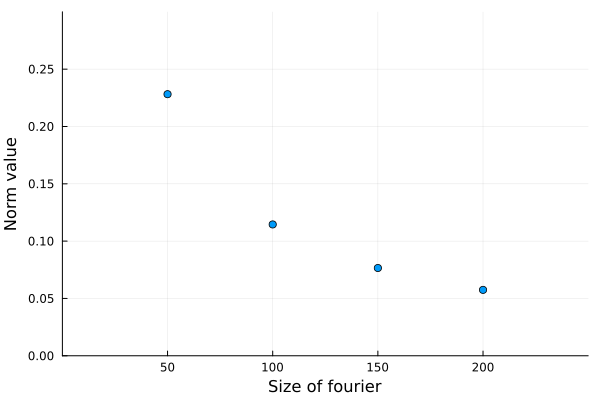
\includegraphics[width=0.8cm,clip]{test.png}
%     \caption{figure_title}
%     \label{fig:hey}
% \end{figure}

\begin{figure}[H]
\centering
\includegraphics[width=0.8\linewidth]{blas512m1024.pdf}
\caption{マシン1の速度比較}
\end{figure}

\begin{figure}[H]
\centering
\includegraphics[width=0.8\linewidth]{blas512m2048.pdf}
\caption{マシン1の速度比較}
\end{figure}

\begin{figure}[H]
\centering
\includegraphics[width=0.8\linewidth]{blas512n1024.pdf}
\caption{マシン1の速度比較}
\end{figure}

\begin{figure}[H]
\centering
\includegraphics[width=0.8\linewidth]{blas512n2048.pdf}
\caption{マシン1の速度比較}
\end{figure}

\begin{figure}[H]
\centering
\includegraphics[width=0.8\linewidth]{blas512k1024.pdf}
\caption{マシン1の速度比較}
\end{figure}

\begin{figure}[H]
\centering
\includegraphics[width=0.8\linewidth]{blas512k2048.pdf}
\caption{マシン1の速度比較}
\end{figure}

\begin{figure}[H]
\centering
\includegraphics[width=0.8\linewidth]{blas1024.pdf}
\caption{マシン1の速度比較}
\end{figure}

\begin{figure}[H]
\centering
\includegraphics[width=0.8\linewidth]{blas1024m512.pdf}
\caption{マシン1の速度比較}
\end{figure}

\begin{figure}[H]
\centering
\includegraphics[width=0.8\linewidth]{blas1024m2048.pdf}
\caption{マシン1の速度比較}
\end{figure}

\begin{figure}[H]
\centering
\includegraphics[width=0.8\linewidth]{blas1024n512.pdf}
\caption{マシン1の速度比較}
\end{figure}

\begin{figure}[H]
\centering
\includegraphics[width=0.8\linewidth]{blas1024n2048.pdf}
\caption{マシン1の速度比較}
\end{figure}

\begin{figure}[H]
\centering
\includegraphics[width=0.8\linewidth]{blas1024k512.pdf}
\caption{マシン1の速度比較}
\end{figure}

\begin{figure}[H]
\centering
\includegraphics[width=0.8\linewidth]{blas1024k2048.pdf}
\caption{マシン1の速度比較}
\end{figure}

\begin{figure}[H]
\centering
\includegraphics[width=0.8\linewidth]{all2048.pdf}
\caption{マシン1の速度比較}
\end{figure}

\begin{figure}[H]
\centering
\includegraphics[width=0.8\linewidth]{all2048,m=512.pdf}
\caption{マシン1の速度比較}
\end{figure}

\begin{figure}[H]
\centering
\includegraphics[width=0.8\linewidth]{all2048,m=1024.pdf}
\caption{マシン1の速度比較}
\end{figure}

\begin{figure}[H]
\centering
\includegraphics[width=0.8\linewidth]{all2048,n=512.pdf}
\caption{マシン1の速度比較}
\end{figure}

\begin{figure}[H]
\centering
\includegraphics[width=0.8\linewidth]{all2048,n=1024.pdf}
\caption{マシン1の速度比較}
\end{figure}

\begin{figure}[H]
\centering
\includegraphics[width=0.8\linewidth]{all2048,k=512.pdf}
\caption{マシン1の速度比較}
\end{figure}

\begin{figure}[H]
\centering
\includegraphics[width=0.8\linewidth]{all2048,k=1024.pdf}
\caption{マシン1の速度比較}
\end{figure}

\begin{figure}[H]
\centering
\includegraphics[width=0.8\linewidth]{b512.pdf}
\caption{$m,n,k = 1024$の計算時間}
\end{figure}

\begin{figure}[H]
\centering
\includegraphics[width=0.8\linewidth]{b512m1024.pdf}
\caption{マシン2の速度比較}
\end{figure}

\begin{figure}[H]
\centering
\includegraphics[width=0.8\linewidth]{b512m2048.pdf}
\caption{マシン2の速度比較}
\end{figure}

\begin{figure}[H]
\centering
\includegraphics[width=0.8\linewidth]{b512n1024.pdf}
\caption{マシン2の速度比較}
\end{figure}

\begin{figure}[H]
\centering
\includegraphics[width=0.8\linewidth]{b512n2048.pdf}
\caption{マシン2の速度比較}
\end{figure}

\begin{figure}[H]
\centering
\includegraphics[width=0.8\linewidth]{b512k1024.pdf}
\caption{マシン2の速度比較}
\end{figure}

\begin{figure}[H]
\centering
\includegraphics[width=0.8\linewidth]{b512k2048.pdf}
\caption{マシン2の速度比較}
\end{figure}

\begin{figure}[H]
\centering
\includegraphics[width=0.8\linewidth]{b1024.pdf}
\caption{マシン2の速度比較}
\end{figure}

\begin{figure}[H]
\centering
\includegraphics[width=0.8\linewidth]{b1024m512.pdf}
\caption{マシン2の速度比較}
\end{figure}

\begin{figure}[H]
\centering
\includegraphics[width=0.8\linewidth]{b1024m2048.pdf}
\caption{マシン2の速度比較}
\end{figure}

\begin{figure}[H]
\centering
\includegraphics[width=0.8\linewidth]{b1024n512.pdf}
\caption{マシン2の速度比較}
\end{figure}

\begin{figure}[H]
\centering
\includegraphics[width=0.8\linewidth]{b1024n2048.pdf}
\caption{マシン2の速度比較}
\end{figure}

\begin{figure}[H]
\centering
\includegraphics[width=0.8\linewidth]{b1024k512.pdf}
\caption{マシン2の速度比較}
\end{figure}

\begin{figure}[H]
\centering
\includegraphics[width=0.8\linewidth]{b1024k2048.pdf}
\caption{マシン2の速度比較}
\end{figure}

\begin{figure}[H]
\centering
\includegraphics[width=0.8\linewidth]{b2048.pdf}
\caption{マシン2の速度比較}
\end{figure}

\begin{figure}[H]
\centering
\includegraphics[width=0.8\linewidth]{b2048m512.pdf}
\caption{マシン2の速度比較}
\end{figure}

\begin{figure}[H]
\centering
\includegraphics[width=0.8\linewidth]{b2048m1024.pdf}
\caption{マシン2の速度比較}
\end{figure}

\begin{figure}[H]
\centering
\includegraphics[width=0.8\linewidth]{b2048n512.pdf}
\caption{マシン2の速度比較}
\end{figure}

\begin{figure}[H]
\centering
\includegraphics[width=0.8\linewidth]{b2048n1024.pdf}
\caption{マシン2の速度比較}
\end{figure}

\begin{figure}[H]
\centering
\includegraphics[width=0.8\linewidth]{b2048k512.pdf}
\caption{マシン2の速度比較}
\end{figure}

\begin{figure}[H]
\centering
\includegraphics[width=0.8\linewidth]{b2048k1024.pdf}
\caption{マシン2の速度比較}
\end{figure}

\indent 次に, マシン1において提案手法とBLASを用いた既存手法に対し, 前節の21パターンの精度を比較したグラフを以下の表5.1から表5.21に示す. 比較する箇所は提案手法と既存手法に対し, 同様の場所を10箇所取り出し, 比較を行う. このときcl,cuはそれぞれ提案手法の結果の区間の上端下端であり, dl,duは既存手法の結果の区間上端下端である.



\begin{table}[H]
\centering
\begin{tabular}{|c|c|c|c|c|}
\hline
& cl & cu & dl & du \\ \hline
1ヵ所目 & -16.82680316 & -16.69964356 & -16.82680617 & -16.69964021 \\ \hline
2ヵ所目 & 13.97806268 & 14.09593355 & 13.97805959 & 14.09593635 \\ \hline
3ヵ所目 & 10.76114969 & 10.89158026 & 10.76114632 & 10.89158341 \\ \hline
4ヵ所目 & -3.095083784 & -2.953419438 & -3.095087295 & -2.953415867 \\ \hline
5ヵ所目 & 7.589419574 & 7.715563773 & 7.589416344 & 7.71556685 \\ \hline
6ヵ所目 & -0.162638825 & -0.02189793 & -0.162642342 & -0.021894411 \\ \hline
7ヵ所目 & -47.90795719 & -47.77695476 & -47.90795999 & -47.77695101 \\ \hline
8ヵ所目 & -31.73850608 & -31.62356277 & -31.73850864 & -31.62355958 \\ \hline
9ヵ所目 & 13.85839284 & 13.99928697 & 13.85838918 & 13.99929036 \\ \hline
10ヵ所目 & -3.755653587 & -3.624137109 & -3.755656838 & -3.624133784 \\ \hline
\end{tabular}
\caption{マシン1の提案手法とBLASを用いた手法との精度比較(パターン1)}
\end{table}

\begin{table}[H]
\centering
\begin{tabular}{|c|c|c|c|c|}
\hline
 & cl & cu & dl & du \\ \hline
1ヵ所目 & -0.960272457 & -0.827787336 & -0.960275759 & -0.827784015 \\ \hline
2ヵ所目 & 31.71398915 & 31.83571311 & 31.71398579 & 31.83571583 \\ \hline
3ヵ所目 & 30.930656 & 31.05464085 & 30.93065259 & 31.05464364 \\ \hline
4ヵ所目 & -16.48339922 & -16.36191128 & -16.48340209 & -16.36190808 \\ \hline
5ヵ所目 & 11.89699213 & 12.02847663 & 11.89698872 & 12.02847979 \\ \hline
6ヵ所目 & 11.82676627 & 11.94748081 & 11.82676314 & 11.94748371 \\ \hline
7ヵ所目 & 4.771796029 & 4.907280988 & 4.771792594 & 4.907284327 \\ \hline
8ヵ所目 & 10.45341597 & 10.5877627 & 10.4534125 & 10.58776595 \\ \hline
9ヵ所目 & 43.35591872 & 43.48529643 & 43.35591505 & 43.48529923 \\ \hline
10ヵ所目 & -20.3503216 & -20.22564619 & -20.35032451 & -20.22564288 \\ \hline
\end{tabular}
\caption{マシン1の提案手法とBLASを用いた手法との精度比較(パターン2)}
\end{table}


\begin{table}[H]
\centering
\begin{tabular}{|c|c|c|c|c|}
\hline
場所 & cl & cu & dl & du \\ \hline
1ヵ所目 & 17.67432195 & 17.8085304 & 17.67431842 & 17.80853358 \\ \hline
2ヵ所目 & 6.804083761 & 6.934655121 & 6.804080429 & 6.934658317 \\ \hline
3ヵ所目 & -11.38945721 & -11.24611736 & -11.38946068 & -11.24611366 \\ \hline
4ヵ所目 & -21.59480126 & -21.46557263 & -21.59480427 & -21.46556919 \\ \hline
5ヵ所目 & 9.76764299 & 9.893373155 & 9.767639749 & 9.893376199 \\ \hline
6ヵ所目 & 17.26147512 & 17.38343486 & 17.26147189 & 17.38343774 \\ \hline
7ヵ所目 & -0.362863015 & -0.233250258 & -0.362866252 & -0.233247015 \\ \hline
8ヵ所目 & -15.3949946 & -15.25686031 & -15.3949979 & -15.2568567 \\ \hline
9ヵ所目 & 18.48171055 & 18.61101731 & 18.48170713 & 18.61102035 \\ \hline
10ヵ所目 & 12.97336827 & 13.10274104 & 12.97336491 & 13.10274415 \\ \hline
\end{tabular}
\caption{マシン1の提案手法とBLASを用いた手法との精度比較(パターン3)}
\end{table}

\begin{table}[H]
\centering
\begin{tabular}{|c|c|c|c|c|}
\hline
場所 & cl & cu & dl & du \\ \hline
1ヵ所目 & -24.64608837 & -24.3736231 & -24.64609494 & -24.37361604 \\ \hline
2ヵ所目 & -49.2723202 & -49.00211223 & -49.27232646 & -49.00210498 \\ \hline
3ヵ所目 & -39.42998777 & -39.15685472 & -39.42999421 & -39.1568475 \\ \hline
4ヵ所目 & -6.844240681 & -6.587096379 & -6.844247042 & -6.587089884 \\ \hline
5ヵ所目 & -39.56085517 & -39.30302234 & -39.56086122 & -39.3030155 \\ \hline
6ヵ所目 & 53.46328097 & 53.72880477 & 53.4632738 & 53.72881087 \\ \hline
7ヵ所目 & -82.54310238 & -82.29164014 & -82.54310785 & -82.29163303 \\ \hline
8ヵ所目 & -2.756812906 & -2.49448142 & -2.756819438 & -2.494474836 \\ \hline
9ヵ所目 & -34.0181092 & -33.75168753 & -34.01811552 & -33.75168053 \\ \hline
10ヵ所目 & 0.150996196 & 0.400642832 & 0.150989953 & 0.400649069 \\ \hline
\end{tabular}
\caption{マシン1の提案手法とBLASを用いた手法との精度比較(パターン4)}
\end{table}

\begin{table}[H]
\centering
\begin{tabular}{|c|c|c|c|c|}
\hline
場所 & cl & cu & dl & du \\ \hline
1ヵ所目 & -6.197135605 & -5.691715522 & -6.19714818 & -5.691702828 \\ \hline
2ヵ所目 & 3.714608079 & 4.219428275 & 3.71459542 & 4.219440854 \\ \hline
3ヵ所目 & 24.63969373 & 25.1706195 & 24.63968021 & 25.17063252 \\ \hline
4ヵ所目 & -88.14774927 & -87.59575208 & -88.14776219 & -87.59573741 \\ \hline
5ヵ所目 & -17.60895729 & -17.0875813 & -17.60897015 & -17.08756809 \\ \hline
6ヵ所目 & 11.80592195 & 12.33259142 & 11.80590866 & 12.33260446 \\ \hline
7ヵ所目 & -15.9673354 & -15.44740901 & -15.96734824 & -15.44739586 \\ \hline
8ヵ所目 & 14.53696663 & 15.05345654 & 14.53695357 & 15.0534693 \\ \hline
9ヵ所目 & -9.505371834 & -8.987268773 & -9.505384693 & -8.98725573 \\ \hline
10ヵ所目 & -72.42306945 & -71.89695703 & -72.42308188 & -71.89694315 \\ \hline
\end{tabular}
\caption{マシン1の提案手法とBLASを用いた手法との精度比較(パターン5)}
\end{table}

\begin{table}[H]
\centering
\begin{tabular}{|c|c|c|c|c|}
\hline
場所 & cl & cu & dl & du \\ \hline
1ヵ所目 & -50.88195895 & -50.75269715 & -50.88196167 & -50.75269341 \\ \hline
2ヵ所目 & 18.49221622 & 18.62240977 & 18.49221278 & 18.62241284 \\ \hline
3ヵ所目 & 26.67423777 & 26.80577206 & 26.67423422 & 26.80577508 \\ \hline
4ヵ所目 & -53.78620294 & -53.66045936 & -53.78620555 & -53.66045568 \\ \hline
5ヵ所目 & -18.94636647 & -18.82116073 & -18.94636941 & -18.82115741 \\ \hline
6ヵ所目 & -6.776461765 & -6.649734609 & -6.776464866 & -6.649731374 \\ \hline
7ヵ所目 & -26.18745111 & -26.05258643 & -26.18745422 & -26.0525828 \\ \hline
8ヵ所目 & 9.44070896 & 9.567538239 & 9.440705694 & 9.567541314 \\ \hline
9ヵ所目 & -32.11439396 & -31.9902608 & -32.11439674 & -31.99025738 \\ \hline
10ヵ所目 & -18.81403993 & -18.68809999 & -18.81404289 & -18.68809665 \\ \hline
\end{tabular}
\caption{マシン1の提案手法とBLASを用いた手法との精度比較(パターン6)}
\end{table}

\begin{table}[H]
\centering
\begin{tabular}{|c|c|c|c|c|}
\hline
場所 & cl & cu & dl & du \\ \hline
1ヵ所目 & 48.37932207 & 48.51084258 & 48.3793183 & 48.51084538 \\ \hline
2ヵ所目 & -11.98296777 & -11.83672405 & -11.98297131 & -11.83672027 \\ \hline
3ヵ所目 & -48.04688372 & -47.90509218 & -48.04688678 & -47.90508815 \\ \hline
4ヵ所目 & -2.288165131 & -2.164240294 & -2.288168207 & -2.164237174 \\ \hline
5ヵ所目 & 24.64525987 & 24.77330298 & 24.64525643 & 24.77330593 \\ \hline
6ヵ所目 & -23.04808881 & -22.9254267 & -23.04809165 & -22.92542341 \\ \hline
7ヵ所目 & -9.11015975 & -8.976625229 & -9.110162998 & -8.976621801 \\ \hline
8ヵ所目 & 41.52354654 & 41.64785548 & 41.52354301 & 41.64785817 \\ \hline
9ヵ所目 & -25.21694588 & -25.08422874 & -25.21694895 & -25.08422517 \\ \hline
10ヵ所目 & 36.18935625 & 36.30887539 & 36.1893529 & 36.30887802 \\ \hline
\end{tabular}
\caption{マシン1の提案手法とBLASを用いた手法との精度比較(パターン7)}
\end{table}

\begin{table}[H]
\centering
\begin{tabular}{|c|c|c|c|c|}
\hline
場所 & cl & cu & dl & du \\ \hline
1ヵ所目 & 18.21254876 & 18.4627439 & 18.21254232 & 18.46274997 \\ \hline
2ヵ所目 & -22.27412814 & -22.02352667 & -22.27413419 & -22.02352019 \\ \hline
3ヵ所目 & 14.29690189 & 14.55456407 & 14.29689531 & 14.55457036 \\ \hline
4ヵ所目 & -17.56955265 & -17.31042337 & -17.56955895 & -17.31041672 \\ \hline
5ヵ所目 & 32.39158594 & 32.65761878 & 32.39157896 & 32.65762511 \\ \hline
6ヵ所目 & 13.10807616 & 13.36136217 & 13.1080697 & 13.36136837 \\ \hline
7ヵ所目 & -19.84766886 & -19.5842545 & -19.84767524 & -19.58424772 \\ \hline
8ヵ所目 & 0.31554348 & 0.581450946 & 0.315536829 & 0.581457589 \\ \hline
9ヵ所目 & 4.876080293 & 5.142032357 & 4.876073595 & 5.142038955 \\ \hline
10ヵ所目 & 16.04859309 & 16.31089177 & 16.04858637 & 16.31089817 \\ \hline
\end{tabular}
\caption{マシン1の提案手法とBLASを用いた手法との精度比較(パターン8)}
\end{table}

\begin{table}[H]
\centering
\begin{tabular}{|c|c|c|c|c|}
\hline
場所 & cl & cu & dl & du \\ \hline
1ヵ所目 & 4.058089528 & 4.316042771 & 4.058083038 & 4.316049177 \\ \hline
2ヵ所目 & -44.03296429 & -43.78336446 & -44.03297009 & -43.78335778 \\ \hline
3ヵ所目 & 33.36308544 & 33.6252792 & 33.36307856 & 33.62528542 \\ \hline
4ヵ所目 & -5.258497714 & -4.994054345 & -5.258504273 & -4.994047683 \\ \hline
5ヵ所目 & -21.10695788 & -20.84632381 & -21.10696419 & -20.84631709 \\ \hline
6ヵ所目 & 7.428483446 & 7.673038407 & 7.428477258 & 7.673044445 \\ \hline
7ヵ所目 & -2.864417957 & -2.61171974 & -2.864424246 & -2.611713396 \\ \hline
8ヵ所目 & -39.28642886 & -39.01866263 & -39.28643516 & -39.01865554 \\ \hline
9ヵ所目 & 58.05456216 & 58.29224415 & 58.05455563 & 58.29224951 \\ \hline
10ヵ所目 & 6.035946737 & 6.293461231 & 6.035940238 & 6.293467607 \\ \hline
\end{tabular}
\caption{マシン1の提案手法とBLASを用いた手法との精度比較(パターン9)}
\end{table}

\begin{table}[H]
\centering
\begin{tabular}{|c|c|c|c|c|}
\hline
場所 & cl & cu & dl & du \\ \hline
1ヵ所目 & -37.67723333 & -37.41913949 & -37.67723941 & -37.41913266 \\ \hline
2ヵ所目 & 43.41784065 & 43.68407502 & 43.41783356 & 43.68408124 \\ \hline
3ヵ所目 & -1.820399608 & -1.560749329 & -1.820406082 & -1.560742822 \\ \hline
4ヵ所目 & -20.20655578 & -19.95608964 & -20.20656184 & -19.95608317 \\ \hline
5ヵ所目 & 45.72290925 & 45.99580844 & 45.72290197 & 45.99581481 \\ \hline
6ヵ所目 & 0.220086634 & 0.465418381 & 0.220080498 & 0.46542451 \\ \hline
7ヵ所目 & -41.33764102 & -41.06658488 & -41.33764739 & -41.0665777 \\ \hline
8ヵ所目 & -3.505757563 & -3.254989229 & -3.505763797 & -3.254982927 \\ \hline
9ヵ所目 & -29.03637491 & -28.77131301 & -29.03638124 & -28.77130609 \\ \hline
10ヵ所目 & 10.21022739 & 10.48910775 & 10.21022031 & 10.48911461 \\ \hline
\end{tabular}
\caption{マシン1の提案手法とBLASを用いた手法との精度比較(パターン10)}
\end{table}

\begin{table}[H]
\centering
\begin{tabular}{|c|c|c|c|c|}
\hline
場所 & cl & cu & dl & du \\ \hline
1ヵ所目 & 47.8371868 & 47.96625897 & 47.8371831 & 47.96626171 \\ \hline
2ヵ所目 & 10.29765208 & 10.42855025 & 10.29764871 & 10.42855342 \\ \hline
3ヵ所目 & -24.846907 & -24.72047375 & -24.84690992 & -24.72047034 \\ \hline
4ヵ所目 & -42.33582926 & -42.20789461 & -42.33583204 & -42.20789099 \\ \hline
5ヵ所目 & -39.28899205 & -39.14673558 & -39.28899521 & -39.14673163 \\ \hline
6ヵ所目 & 37.36636452 & 37.50170111 & 37.36636076 & 37.50170411 \\ \hline
7ヵ所目 & 16.69040232 & 16.82931815 & 16.69039868 & 16.82932146 \\ \hline
8ヵ所目 & 15.8072126 & 15.92694112 & 15.80720945 & 15.92694396 \\ \hline
9ヵ所目 & 0.530143674 & 0.656667976 & 0.530140505 & 0.656671133 \\ \hline
10ヵ所目 & 7.811975676 & 7.928543494 & 7.811972683 & 7.928546329 \\ \hline
\end{tabular}
\caption{マシン1の提案手法とBLASを用いた手法との精度比較(パターン11)}
\end{table}

\begin{table}[H]
\centering
\begin{tabular}{|c|c|c|c|c|}
\hline
場所 & cl & cu & dl & du \\ \hline
1ヵ所目 & -51.9765984 & -51.46373357 & -51.97661071 & -51.46372023 \\ \hline
2ヵ所目 & -42.87993787 & -42.35967884 & -42.87995045 & -42.35966541 \\ \hline
3ヵ所目 & -4.40108803 & -3.879720479 & -4.401101022 & -3.879707405 \\ \hline
4ヵ所目 & -23.87567143 & -23.3594914 & -23.8756841 & -23.35947826 \\ \hline
5ヵ所目 & 24.06004132 & 24.5919453 & 24.06002778 & 24.59195836 \\ \hline
6ヵ所目 & 37.65509456 & 38.16817136 & 37.65508135 & 38.16818381 \\ \hline
7ヵ所目 & -12.61070037 & -12.09453939 & -12.61071315 & -12.09452636 \\ \hline
8ヵ所目 & 33.16602384 & 33.67992776 & 33.16601066 & 33.67994027 \\ \hline
9ヵ所目 & 39.35283694 & 39.86597063 & 39.35282371 & 39.86598306 \\ \hline
10ヵ所目 & -18.53965038 & -18.01534085 & -18.5396633 & -18.01532757 \\ \hline
\end{tabular}
\caption{マシン1の提案手法とBLASを用いた手法との精度比較(パターン12)}
\end{table}

\begin{table}[H]
\centering
\begin{tabular}{|c|c|c|c|c|}
\hline
場所 & cl & cu & dl & du \\ \hline
1ヵ所目 & -28.42593248 & -28.15626626 & -28.42593893 & -28.15625924 \\ \hline
2ヵ所目 & -13.38311415 & -13.13406979 & -13.38312024 & -13.13406343 \\ \hline
3ヵ所目 & -25.36435652 & -25.11646907 & -25.36436247 & -25.11646262 \\ \hline
4ヵ所目 & -25.92386542 & -25.66425364 & -25.92387165 & -25.66424689 \\ \hline
5ヵ所目 & -5.966944902 & -5.728955695 & -5.966950793 & -5.728949687 \\ \hline
6ヵ所目 & 1.163409615 & 1.432557169 & 1.163402875 & 1.432563884 \\ \hline
7ヵ所目 & -34.39663288 & -34.14060809 & -34.39663894 & -34.14060135 \\ \hline
8ヵ所目 & -59.43788396 & -59.18739826 & -59.43788963 & -59.1873914 \\ \hline
9ヵ所目 & -63.29104867 & -63.04630598 & -63.29105416 & -63.04629923 \\ \hline
10ヵ所目 & -34.35449371 & -34.10724634 & -34.35449954 & -34.10723982 \\ \hline
\end{tabular}
\caption{マシン1の提案手法とBLASを用いた手法との精度比較(パターン13)}
\end{table}


\begin{table}[H]
\centering
\begin{tabular}{|c|c|c|c|c|}
\hline
場所 & cl & cu & dl & du \\ \hline
1ヵ所目 & 7.758149091 & 8.018063168 & 7.758142515 & 8.018069586 \\ \hline
2ヵ所目 & 0.494956132 & 0.751917883 & 0.494949703 & 0.7519243 \\ \hline
3ヵ所目 & 23.94433027 & 24.2165088 & 23.94432322 & 24.21651536 \\ \hline
4ヵ所目 & -20.8306556 & -20.56980848 & -20.83066192 & -20.56980175 \\ \hline
5ヵ所目 & 14.9962195 & 15.25850647 & 14.99621279 & 15.25851288 \\ \hline
6ヵ所目 & 59.48724304 & 59.75880098 & 59.48723566 & 59.75880718 \\ \hline
7ヵ所目 & 1.255892285 & 1.520605088 & 1.255885654 & 1.520611692 \\ \hline
8ヵ所目 & 27.75672951 & 28.0153774 & 27.75672276 & 28.01538359 \\ \hline
9ヵ所目 & 57.99597473 & 58.24004762 & 57.99596805 & 58.24005314 \\ \hline
10ヵ所目 & -24.35651137 & -24.10130223 & -24.3565175 & -24.10129561 \\ \hline
\end{tabular}
\caption{マシン1の提案手法とBLASを用いた手法との精度比較(パターン14)}
\end{table}

\begin{table}[H]
\centering
\begin{tabular}{|c|c|c|c|c|}
\hline
場所 & cl & cu & dl & du \\ \hline
1ヵ所目 & -53.02624507 & -52.49926832 & -53.02625772 & -52.49925462 \\ \hline
2ヵ所目 & 10.32814282 & 10.8719105 & 10.32812912 & 10.87192399 \\ \hline
3ヵ所目 & -3.57576048 & -3.057071442 & -3.575773413 & -3.057058442 \\ \hline
4ヵ所目 & 45.6570358 & 46.19486807 & 45.65702189 & 46.19488105 \\ \hline
5ヵ所目 & 3.300599212 & 3.83772147 & 3.300585749 & 3.837734861 \\ \hline
6ヵ所目 & -32.34521533 & -31.82035761 & -32.34522813 & -31.82034417 \\ \hline
7ヵ所目 & 22.82011914 & 23.33697324 & 22.82010599 & 23.33698593 \\ \hline
8ヵ所目 & 41.10792054 & 41.62229938 & 41.10790726 & 41.62231182 \\ \hline
9ヵ所目 & 76.45743094 & 76.98160748 & 76.45741707 & 76.98161982 \\ \hline
10ヵ所目 & 0.552407272 & 1.07752887 & 0.552394137 & 1.077541989 \\ \hline
\end{tabular}
\caption{マシン1の提案手法とBLASを用いた手法との精度比較(パターン15)}
\end{table}

\begin{table}[H]
\centering
\begin{tabular}{|c|c|c|c|c|}
\hline
場所 & cl & cu & dl & du \\ \hline
1ヵ所目 & -15.85286001 & -15.3414796 & -15.85287264 & -15.34146666 \\ \hline
2ヵ所目 & 47.0493142 & 47.56298787 & 47.04930089 & 47.56300024 \\ \hline
3ヵ所目 & -14.36685625 & -13.8767175 & -14.36686836 & -13.87670511 \\ \hline
4ヵ所目 & -34.37669213 & -33.847734 & -34.37670501 & -33.84772043 \\ \hline
5ヵ所目 & 22.29835539 & 22.80536361 & 22.29834249 & 22.80537606 \\ \hline
6ヵ所目 & -15.19085526 & -14.65964581 & -15.19086839 & -14.65963238 \\ \hline
7ヵ所目 & -14.27052507 & -13.77400243 & -14.27053734 & -13.77398988 \\ \hline
8ヵ所目 & -53.59792312 & -53.08032655 & -53.59793552 & -53.08031308 \\ \hline
9ヵ所目 & 22.16012817 & 22.68835641 & 22.16011474 & 22.68836939 \\ \hline
10ヵ所目 & 66.36592362 & 66.89404682 & 66.36590976 & 66.89405936 \\ \hline
\end{tabular}
\caption{マシン1の提案手法とBLASを用いた手法との精度比較(パターン16)}
\end{table}

\begin{table}[H]
\centering
\begin{tabular}{|c|c|c|c|c|}
\hline
場所 & cl & cu & dl & du \\ \hline
1ヵ所目 & 7.896650957 & 8.412424742 & 7.896637983 & 8.412437554 \\ \hline
2ヵ所目 & -18.80074066 & -18.26812096 & -18.80075379 & -18.26810746 \\ \hline
3ヵ所目 & -34.80336321 & -34.25834209 & -34.80337649 & -34.25832812 \\ \hline
4ヵ所目 & 0.15849485 & 0.696120888 & 0.158481406 & 0.696134323 \\ \hline
5ヵ所目 & 77.88139147 & 78.4393744 & 77.88137674 & 78.43938757 \\ \hline
6ヵ所目 & -81.85776625 & -81.33878139 & -81.85777841 & -81.3387676 \\ \hline
7ヵ所目 & 49.93842631 & 50.48327072 & 49.93841219 & 50.48328384 \\ \hline
8ヵ所目 & -0.683076887 & -0.164258807 & -0.683089852 & -0.164245834 \\ \hline
9ヵ所目 & 25.62317933 & 26.1120839 & 25.62316685 & 26.11209586 \\ \hline
10ヵ所目 & 59.21080405 & 59.73887191 & 59.21079025 & 59.73888452 \\ \hline
\end{tabular}
\caption{マシン1の提案手法とBLASを用いた手法との精度比較(パターン17)}
\end{table}

\begin{table}[H]
\centering
\begin{tabular}{|c|c|c|c|c|}
\hline
場所 & cl & cu & dl & du \\ \hline
1ヵ所目 & -34.8738953 & -34.74596562 & -34.87389815 & -34.74596207 \\ \hline
2ヵ所目 & 28.81297674 & 28.93152393 & 28.81297349 & 28.9315266 \\ \hline
3ヵ所目 & -42.6429758 & -42.50141392 & -42.64297891 & -42.50140995 \\ \hline
4ヵ所目 & -8.864123675 & -8.742495076 & -8.864126627 & -8.742491947 \\ \hline
5ヵ所目 & -14.03721694 & -13.89467639 & -14.03722036 & -13.89467268 \\ \hline
6ヵ所目 & -19.08183389 & -18.9567485 & -19.08183683 & -18.95674519 \\ \hline
7ヵ所目 & 3.946689388 & 4.076992603 & 3.94668609 & 4.07699582 \\ \hline
8ヵ所目 & 9.700208764 & 9.829123919 & 9.700205443 & 9.829127044 \\ \hline
9ヵ所目 & 28.73828365 & 28.87305784 & 28.73827999 & 28.87306092 \\ \hline
10ヵ所目 & -18.29771639 & -18.15833 & -18.2977197 & -18.15832633 \\ \hline
\end{tabular}
\caption{マシン1の提案手法とBLASを用いた手法との精度比較(パターン18)}
\end{table}

\begin{table}[H]
\centering
\begin{tabular}{|c|c|c|c|c|}
\hline
場所 & cl & cu & dl & du \\ \hline
1ヵ所目 & 10.91098527 & 11.17356447 & 10.91097859 & 11.17357093 \\ \hline
2ヵ所目 & 35.05598953 & 35.32376122 & 35.05598249 & 35.32376756 \\ \hline
3ヵ所目 & 41.08677867 & 41.34986317 & 41.08677168 & 41.34986933 \\ \hline
4ヵ所目 & 11.87738173 & 12.1345975 & 11.87737518 & 12.13460381 \\ \hline
5ヵ所目 & -19.52887225 & -19.26676617 & -19.52887861 & -19.26675943 \\ \hline
6ヵ所目 & -22.96472383 & -22.7043789 & -22.96473011 & -22.70437216 \\ \hline
7ヵ所目 & -2.105005492 & -1.838685242 & -2.10501213 & -1.838678565 \\ \hline
8ヵ所目 & 31.52889924 & 31.77695901 & 31.52889272 & 31.77696489 \\ \hline
9ヵ所目 & 55.28516235 & 55.54662477 & 55.28515526 & 55.54663076 \\ \hline
10ヵ所目 & -17.9782392 & -17.72335591 & -17.9782454 & -17.72334936 \\ \hline
\end{tabular}
\caption{マシン1の提案手法とBLASを用いた手法との精度比較(パターン19)}
\end{table}

\begin{table}[H]
\centering
\begin{tabular}{|c|c|c|c|c|}
\hline
場所 & cl & cu & dl & du \\ \hline
1ヵ所目 & -15.52122736 & -14.97003055 & -15.52124099 & -14.97001662 \\ \hline
2ヵ所目 & -32.21550214 & -31.68774611 & -32.21551501 & -31.6877326 \\ \hline
3ヵ所目 & 45.90961676 & 46.44126385 & 45.90960301 & 46.44127668 \\ \hline
4ヵ所目 & -53.20279218 & -52.69274194 & -53.2028044 & -52.69272866 \\ \hline
5ヵ所目 & 69.14844817 & 69.62727804 & 69.14843551 & 69.62728931 \\ \hline
6ヵ所目 & 48.01735517 & 48.5304932 & 48.01734186 & 48.53050554 \\ \hline
7ヵ所目 & 90.73742204 & 91.27292845 & 90.73740774 & 91.27294092 \\ \hline
8ヵ所目 & 24.14726382 & 24.67205914 & 24.14725046 & 24.67207201 \\ \hline
9ヵ所目 & -74.92480098 & -74.38533734 & -74.92481372 & -74.3853231 \\ \hline
10ヵ所目 & 2.914886134 & 3.433892613 & 2.914873128 & 3.433905555 \\ \hline
\end{tabular}
\caption{マシン1の提案手法とBLASを用いた手法との精度比較(パターン20)}
\end{table}

\begin{table}[H]
\centering
\begin{tabular}{|c|c|c|c|c|}
\hline
場所 & cl & cu & dl & du \\ \hline
1ヵ所目 & 82.62686318 & 83.14335149 & 82.62684944 & 83.14336357 \\ \hline
2ヵ所目 & -50.04988143 & -49.54241015 & -50.04989362 & -49.54239697 \\ \hline
3ヵ所目 & -69.82845176 & -69.31170261 & -69.82846398 & -69.311689 \\ \hline
4ヵ所目 & -64.81374011 & -64.27090294 & -64.81375304 & -64.27088872 \\ \hline
5ヵ所目 & -51.69241999 & -51.15917054 & -51.69243281 & -51.1591567 \\ \hline
6ヵ所目 & 20.91118197 & 21.42474816 & 20.91116892 & 21.42476079 \\ \hline
7ヵ所目 & 46.31442068 & 46.83263196 & 46.31440726 & 46.83264445 \\ \hline
8ヵ所目 & -54.77040622 & -54.24990182 & -54.77041869 & -54.24988826 \\ \hline
9ヵ所目 & -3.215385725 & -2.695227212 & -3.215398699 & -2.69521418 \\ \hline
10ヵ所目 & -8.805947165 & -8.29459516 & -8.805959862 & -8.294582292 \\ \hline
\end{tabular}
\caption{マシン1の提案手法とBLASを用いた手法との精度比較(パターン21)}
\end{table}


\indent 次に, マシン1,において提案手法と区間積和演算を計算する既存手法に対し, 前節の21パターンの精度を比較したグラフを以下の表5.22から表5.42に示す. また同様に比較する箇所は同じ個所を取り出し, 比較する.cl,cu,dl,duも同様に提案手法と既存手法の結果の区間の上端下端とする.

\begin{table}[H]
\centering
\begin{tabular}{|c|c|c|c|c|}
\hline
場所 & cl & cu & dl & du \\ \hline
1ヵ所目 & -23.52726816 & -23.40746494 & -23.52726816 & -23.40746494 \\ \hline
2ヵ所目 & -9.772786958 & -9.639098696 & -9.772786958 & -9.639098696 \\ \hline
3ヵ所目 & 14.04268654 & 14.1755164 & 14.04268654 & 14.1755164 \\ \hline
4ヵ所目 & 20.58901349 & 20.71482842 & 20.58901349 & 20.71482842 \\ \hline
5ヵ所目 & -34.26528711 & -34.1280351 & -34.26528711 & -34.1280351 \\ \hline
6ヵ所目 & -7.718818703 & -7.584056419 & -7.718818703 & -7.584056419 \\ \hline
7ヵ所目 & 7.287899267 & 7.405781626 & 7.287899267 & 7.405781626 \\ \hline
8ヵ所目 & -45.63106205 & -45.5007445 & -45.63106205 & -45.5007445 \\ \hline
9ヵ所目 & -2.135874663 & -2.001688501 & -2.135874663 & -2.001688501 \\ \hline
10ヵ所目 & -8.636260533 & -8.51073305 & -8.636260533 & -8.51073305 \\ \hline
\end{tabular}
\caption{マシン1の提案手法と区間積和演算を計算する手法との精度比較(パターン1)}
\end{table}

\begin{table}[H]
\centering
\begin{tabular}{|c|c|c|c|c|}
\hline
場所 & cl & cu & dl & du \\ \hline
1ヵ所目 & 2.927307704 & 3.056266342 & 2.927307704 & 3.056266342 \\ \hline
2ヵ所目 & -9.754077067 & -9.615251613 & -9.754077067 & -9.615251613 \\ \hline
3ヵ所目 & 11.22022266 & 11.34891886 & 11.22022266 & 11.34891886 \\ \hline
4ヵ所目 & -5.832022084 & -5.696988228 & -5.832022084 & -5.696988228 \\ \hline
5ヵ所目 & 4.529250727 & 4.665157808 & 4.529250727 & 4.665157808 \\ \hline
6ヵ所目 & 0.616141163 & 0.748186294 & 0.616141163 & 0.748186294 \\ \hline
7ヵ所目 & -37.5641184 & -37.4210892 & -37.5641184 & -37.4210892 \\ \hline
8ヵ所目 & 13.88055042 & 14.01154043 & 13.88055042 & 14.01154043 \\ \hline
9ヵ所目 & -29.43604573 & -29.30347876 & -29.43604573 & -29.30347876 \\ \hline
10ヵ所目 & 18.87252128 & 18.99974008 & 18.87252128 & 18.99974008 \\ \hline
\end{tabular}
\caption{マシン1の提案手法と区間積和演算を計算する手法との精度比較(パターン2)}
\end{table}

\begin{table}[H]
\centering
\begin{tabular}{|c|c|c|c|c|}
\hline
場所 & cl & cu & dl & du \\ \hline
1ヵ所目 & 21.3890115 & 21.53761924 & 21.3890115 & 21.53761924 \\ \hline
2ヵ所目 & 18.52756469 & 18.65503523 & 18.52756469 & 18.65503523 \\ \hline
3ヵ所目 & -4.14394485 & -4.01086729 & -4.14394485 & -4.01086729 \\ \hline
4ヵ所目 & 2.972044448 & 3.112040173 & 2.972044448 & 3.112040173 \\ \hline
5ヵ所目 & 15.63187191 & 15.76965099 & 15.63187191 & 15.76965099 \\ \hline
6ヵ所目 & -18.96327976 & -18.83448064 & -18.96327976 & -18.83448064 \\ \hline
7ヵ所目 & 0.156361404 & 0.294874002 & 0.156361404 & 0.294874002 \\ \hline
8ヵ所目 & 12.27513035 & 12.40115865 & 12.27513035 & 12.40115865 \\ \hline
9ヵ所目 & -44.88328167 & -44.75205245 & -44.88328167 & -44.75205245 \\ \hline
10ヵ所目 & -35.23002547 & -35.09540885 & -35.23002547 & -35.09540885 \\ \hline
\end{tabular}
\caption{マシン1の提案手法と区間積和演算を計算する手法との精度比較(パターン3)}
\end{table}

\begin{table}[H]
\centering
\begin{tabular}{|c|c|c|c|c|}
\hline
場所 & cl & cu & dl & du \\ \hline
1ヵ所目 & 0.650925249 & 0.90180928 & 0.650925249 & 0.90180928 \\ \hline
2ヵ所目 & -44.11555901 & -43.84214511 & -44.11555901 & -43.84214511 \\ \hline
3ヵ所目 & -57.72373132 & -57.44620563 & -57.72373132 & -57.44620563 \\ \hline
4ヵ所目 & 5.377076719 & 5.635506857 & 5.377076719 & 5.635506857 \\ \hline
5ヵ所目 & -31.80136965 & -31.55064135 & -31.80136965 & -31.55064135 \\ \hline
6ヵ所目 & 25.85343089 & 26.11227412 & 25.85343089 & 26.11227412 \\ \hline
7ヵ所目 & -27.58755904 & -27.32273851 & -27.58755904 & -27.32273851 \\ \hline
8ヵ所目 & 2.890340765 & 3.136890829 & 2.890340765 & 3.136890829 \\ \hline
9ヵ所目 & -12.24771396 & -11.98749711 & -12.24771396 & -11.98749711 \\ \hline
10ヵ所目 & -13.51617661 & -13.25079433 & -13.51617661 & -13.25079433 \\ \hline
\end{tabular}
\caption{マシン1の提案手法と区間積和演算を計算する手法との精度比較(パターン4)}
\end{table}

\begin{table}[H]
\centering
\begin{tabular}{|c|c|c|c|c|}
\hline
場所 & cl & cu & dl & du \\ \hline
1ヵ所目 & -8.108702117 & -7.585345264 & -8.108702117 & -7.585345264 \\ \hline
2ヵ所目 & -15.01174667 & -14.48675763 & -15.01174667 & -14.48675763 \\ \hline
3ヵ所目 & -47.89102232 & -47.37402366 & -47.89102232 & -47.37402366 \\ \hline
4ヵ所目 & -60.97893274 & -60.46617509 & -60.97893274 & -60.46617509 \\ \hline
5ヵ所目 & 7.567778727 & 8.119359536 & 7.567778727 & 8.119359536 \\ \hline
6ヵ所目 & 46.23507528 & 46.7598108 & 46.23507528 & 46.7598108 \\ \hline
7ヵ所目 & -13.14707783 & -12.63523481 & -13.14707783 & -12.63523481 \\ \hline
8ヵ所目 & -22.68513001 & -22.16408458 & -22.68513001 & -22.16408458 \\ \hline
9ヵ所目 & -40.24133797 & -39.68917015 & -40.24133797 & -39.68917015 \\ \hline
10ヵ所目 & 45.7126938 & 46.23689273 & 45.7126938 & 46.23689273 \\ \hline
\end{tabular}
\caption{マシン1の提案手法と区間積和演算を計算する手法との精度比較(パターン5)}
\end{table}

\begin{table}[H]
\centering
\begin{tabular}{|c|c|c|c|c|}
\hline
場所 & cl & cu & dl & du \\ \hline
1ヵ所目 & 33.95402121 & 34.09091856 & 33.95402121 & 34.09091856 \\ \hline
2ヵ所目 & -37.73902779 & -37.60924243 & -37.73902779 & -37.60924243 \\ \hline
3ヵ所目 & -10.37826082 & -10.25687634 & -10.37826082 & -10.25687634 \\ \hline
4ヵ所目 & -5.876424415 & -5.752362848 & -5.876424415 & -5.752362848 \\ \hline
5ヵ所目 & -25.38298366 & -25.25185975 & -25.38298366 & -25.25185975 \\ \hline
6ヵ所目 & 47.30168483 & 47.43393699 & 47.30168483 & 47.43393699 \\ \hline
7ヵ所目 & 12.4741659 & 12.59410316 & 12.4741659 & 12.59410316 \\ \hline
8ヵ所目 & -40.06870347 & -39.94249589 & -40.06870347 & -39.94249589 \\ \hline
9ヵ所目 & -1.237301604 & -1.095904357 & -1.237301604 & -1.095904357 \\ \hline
10ヵ所目 & 20.69615565 & 20.82559972 & 20.69615565 & 20.82559972 \\ \hline
\end{tabular}
\caption{マシン1の提案手法と区間積和演算を計算する手法との精度比較(パターン6)}
\end{table}

\begin{table}[H]
\centering
\begin{tabular}{|c|c|c|c|c|}
\hline
場所 & cl & cu & dl & du \\ \hline
1ヵ所目 & -15.73446554 & -15.59439961 & -15.73446554 & -15.59439961 \\ \hline
2ヵ所目 & 24.70362364 & 24.83142415 & 24.70362364 & 24.83142415 \\ \hline
3ヵ所目 & 59.5978885 & 59.72959109 & 59.5978885 & 59.72959109 \\ \hline
4ヵ所目 & -18.11383605 & -17.97057555 & -18.11383605 & -17.97057555 \\ \hline
5ヵ所目 & -3.792999325 & -3.66483804 & -3.792999325 & -3.66483804 \\ \hline
6ヵ所目 & -21.08607291 & -20.94660089 & -21.08607291 & -20.94660089 \\ \hline
7ヵ所目 & -54.91296483 & -54.77263889 & -54.91296483 & -54.77263889 \\ \hline
8ヵ所目 & 31.66041251 & 31.79918418 & 31.66041251 & 31.79918418 \\ \hline
9ヵ所目 & 33.92292927 & 34.05028134 & 33.92292927 & 34.05028134 \\ \hline
10ヵ所目 & 23.29056094 & 23.42867683 & 23.29056094 & 23.42867683 \\ \hline
\end{tabular}
\caption{マシン1の提案手法と区間積和演算を計算する手法との精度比較(パターン7)}
\end{table}

\begin{table}[H]
\centering
\begin{tabular}{|c|c|c|c|c|}
\hline
場所 & cl & cu & dl & du \\ \hline
1ヵ所目 & -13.01599754 & -12.76507808 & -13.01599754 & -12.76507808 \\ \hline
2ヵ所目 & 13.48838132 & 13.73751726 & 13.48838132 & 13.73751726 \\ \hline
3ヵ所目 & 67.91664899 & 68.1682811 & 67.91664899 & 68.1682811 \\ \hline
4ヵ所目 & -63.9973832 & -63.73980289 & -63.9973832 & -63.73980289 \\ \hline
5ヵ所目 & 19.99314755 & 20.24758582 & 19.99314755 & 20.24758582 \\ \hline
6ヵ所目 & 14.94060592 & 15.20562919 & 14.94060592 & 15.20562919 \\ \hline
7ヵ所目 & 22.29924369 & 22.56421336 & 22.29924369 & 22.56421336 \\ \hline
8ヵ所目 & -4.454831047 & -4.187350154 & -4.454831047 & -4.187350154 \\ \hline
9ヵ所目 & 27.56412809 & 27.82626992 & 27.56412809 & 27.82626992 \\ \hline
10ヵ所目 & -17.18966318 & -16.93442803 & -17.18966318 & -16.93442803 \\ \hline
\end{tabular}
\caption{マシン1の提案手法と区間積和演算を計算する手法との精度比較(パターン8)}
\end{table}

\begin{table}[H]
\centering
\begin{tabular}{|c|c|c|c|c|}
\hline
場所 & cl & cu & dl & du \\ \hline
1ヵ所目 & -13.01599754 & -12.76507808 & -13.01599754 & -12.76507808 \\ \hline
2ヵ所目 & 13.48838132 & 13.73751726 & 13.48838132 & 13.73751726 \\ \hline
3ヵ所目 & 67.91664899 & 68.1682811 & 67.91664899 & 68.1682811 \\ \hline
4ヵ所目 & -63.9973832 & -63.73980289 & -63.9973832 & -63.73980289 \\ \hline
5ヵ所目 & 19.99314755 & 20.24758582 & 19.99314755 & 20.24758582 \\ \hline
6ヵ所目 & 14.94060592 & 15.20562919 & 14.94060592 & 15.20562919 \\ \hline
7ヵ所目 & 22.29924369 & 22.56421336 & 22.29924369 & 22.56421336 \\ \hline
8ヵ所目 & -4.454831047 & -4.187350154 & -4.454831047 & -4.187350154 \\ \hline
9ヵ所目 & 27.56412809 & 27.82626992 & 27.56412809 & 27.82626992 \\ \hline
10ヵ所目 & -17.18966318 & -16.93442803 & -17.18966318 & -16.93442803 \\ \hline
\end{tabular}
\caption{マシン1の提案手法と区間積和演算を計算する手法との精度比較(パターン9)}
\end{table}

\begin{table}[H]
\centering
\begin{tabular}{|c|c|c|c|c|}
\hline
場所 & cl & cu & dl & du \\ \hline
1ヵ所目 & 39.52595968 & 39.78914383 & 39.52595968 & 39.78914383 \\ \hline
2ヵ所目 & 19.37697127 & 19.6241616 & 19.37697127 & 19.6241616 \\ \hline
3ヵ所目 & -25.00473396 & -24.74317291 & -25.00473396 & -24.74317291 \\ \hline
4ヵ所目 & 9.265530906 & 9.549994528 & 9.265530906 & 9.549994528 \\ \hline
5ヵ所目 & -78.43322181 & -78.15807861 & -78.43322181 & -78.15807861 \\ \hline
6ヵ所目 & -14.82792676 & -14.56476563 & -14.82792676 & -14.56476563 \\ \hline
7ヵ所目 & -5.539168239 & -5.280365201 & -5.539168239 & -5.280365201 \\ \hline
8ヵ所目 & 4.51464562 & 4.787197666 & 4.51464562 & 4.787197666 \\ \hline
9ヵ所目 & -30.13418286 & -29.86847465 & -30.13418286 & -29.86847465 \\ \hline
10ヵ所目 & -3.702267952 & -3.423884564 & -3.702267952 & -3.423884564 \\ \hline
\end{tabular}
\caption{マシン1の提案手法と区間積和演算を計算する手法との精度比較(パターン10)}
\end{table}

\begin{table}[H]
\centering
\begin{tabular}{|c|c|c|c|c|}
\hline
場所 & cl & cu & dl & du \\ \hline
1ヵ所目 & -13.70328918 & -13.57856255 & -13.70328918 & -13.57856255 \\ \hline
2ヵ所目 & -8.686786391 & -8.564663492 & -8.686786391 & -8.564663492 \\ \hline
3ヵ所目 & -0.531688585 & -0.402175407 & -0.531688585 & -0.402175407 \\ \hline
4ヵ所目 & 48.10408572 & 48.24299113 & 48.10408572 & 48.24299113 \\ \hline
5ヵ所目 & -21.73711507 & -21.61138869 & -21.73711507 & -21.61138869 \\ \hline
6ヵ所目 & -20.90955165 & -20.78036598 & -20.90955165 & -20.78036598 \\ \hline
7ヵ所目 & -6.417424693 & -6.287152012 & -6.417424693 & -6.287152012 \\ \hline
8ヵ所目 & 3.511025787 & 3.631526311 & 3.511025787 & 3.631526311 \\ \hline
9ヵ所目 & -14.73336276 & -14.59963784 & -14.73336276 & -14.59963784 \\ \hline
10ヵ所目 & 15.10227399 & 15.24038654 & 15.10227399 & 15.24038654 \\ \hline
\end{tabular}
\caption{マシン1の提案手法と区間積和演算を計算する手法との精度比較(パターン11)}
\end{table}

\begin{table}[H]
\centering
\begin{tabular}{|c|c|c|c|c|}
\hline
場所 & cl & cu & dl & du \\ \hline
1ヵ所目 & -67.77602286 & -67.25254985 & -67.77602286 & -67.25254985 \\ \hline
2ヵ所目 & -77.68028678 & -77.1513441 & -77.68028678 & -77.1513441 \\ \hline
3ヵ所目 & 83.81573119 & 84.35466596 & 83.81573119 & 84.35466596 \\ \hline
4ヵ所目 & -6.326876462 & -5.801049347 & -6.326876462 & -5.801049347 \\ \hline
5ヵ所目 & 43.69378336 & 44.21449117 & 43.69378336 & 44.21449117 \\ \hline
6ヵ所目 & -86.52882576 & -86.00212542 & -86.52882576 & -86.00212542 \\ \hline
7ヵ所目 & -44.37924562 & -43.85043014 & -44.37924562 & -43.85043014 \\ \hline
8ヵ所目 & 22.71369917 & 23.23207608 & 22.71369917 & 23.23207608 \\ \hline
9ヵ所目 & 26.94556935 & 27.47964621 & 26.94556935 & 27.47964621 \\ \hline
10ヵ所目 & 3.70147774 & 4.227510461 & 3.70147774 & 4.227510461 \\ \hline
\end{tabular}
\caption{マシン1の提案手法と区間積和演算を計算する手法との精度比較(パターン12)}
\end{table}

\begin{table}[H]
\centering
\begin{tabular}{|c|c|c|c|c|}
\hline
場所 & cl & cu & dl & du \\ \hline
1ヵ所目 & 46.85509771 & 47.10510525 & 46.85509771 & 47.10510525 \\ \hline
2ヵ所目 & -19.48381479 & -19.2259308 & -19.48381479 & -19.2259308 \\ \hline
3ヵ所目 & 19.29591125 & 19.54517667 & 19.29591125 & 19.54517667 \\ \hline
4ヵ所目 & -33.02918865 & -32.76172422 & -33.02918865 & -32.76172422 \\ \hline
5ヵ所目 & -17.95655726 & -17.70249299 & -17.95655726 & -17.70249299 \\ \hline
6ヵ所目 & -0.427444136 & -0.169306532 & -0.427444136 & -0.169306532 \\ \hline
7ヵ所目 & -24.467903 & -24.22314601 & -24.467903 & -24.22314601 \\ \hline
8ヵ所目 & 41.22364526 & 41.49260687 & 41.22364526 & 41.49260687 \\ \hline
9ヵ所目 & -11.74106531 & -11.4806667 & -11.74106531 & -11.4806667 \\ \hline
10ヵ所目 & -3.561835328 & -3.308177806 & -3.561835328 & -3.308177806 \\ \hline
\end{tabular}
\caption{マシン1の提案手法と区間積和演算を計算する手法との精度比較(パターン13)}
\end{table}



\begin{table}[H]
\centering
\begin{tabular}{|c|c|c|c|c|}
\hline
場所 & cl & cu & dl & du \\ \hline
1ヵ所目 & -13.01024772 & -12.76035079 & -13.01024772 & -12.76035079 \\ \hline
2ヵ所目 & 45.48888772 & 45.75715007 & 45.48888772 & 45.75715007 \\ \hline
3ヵ所目 & 55.74483128 & 56.00373806 & 55.74483128 & 56.00373806 \\ \hline
4ヵ所目 & 18.96594843 & 19.23766326 & 18.96594843 & 19.23766326 \\ \hline
5ヵ所目 & 20.70101972 & 20.97298434 & 20.70101972 & 20.97298434 \\ \hline
6ヵ所目 & 50.16913469 & 50.42520965 & 50.16913469 & 50.42520965 \\ \hline
7ヵ所目 & -29.95146123 & -29.7032241 & -29.95146123 & -29.7032241 \\ \hline
8ヵ所目 & 76.71544646 & 76.98175756 & 76.71544646 & 76.98175756 \\ \hline
9ヵ所目 & 8.804160097 & 9.072455263 & 8.804160097 & 9.072455263 \\ \hline
10ヵ所目 & -19.2393995 & -18.96651543 & -19.2393995 & -18.96651543 \\ \hline
\end{tabular}
\caption{マシン1の提案手法と区間積和演算を計算する手法との精度比較(パターン14)}
\end{table}

\begin{table}[H]
\centering
\begin{tabular}{|c|c|c|c|c|}
\hline
場所 & cl & cu & dl & du \\ \hline
1ヵ所目 & -9.885966651 & -9.361430718 & -9.885966651 & -9.361430718 \\ \hline
2ヵ所目 & 2.401272701 & 2.963939143 & 2.401272701 & 2.963939143 \\ \hline
3ヵ所目 & 11.01727057 & 11.55410236 & 11.01727057 & 11.55410236 \\ \hline
4ヵ所目 & 24.97182732 & 25.48440988 & 24.97182732 & 25.48440988 \\ \hline
5ヵ所目 & -32.86046943 & -32.33888251 & -32.86046943 & -32.33888251 \\ \hline
6ヵ所目 & 47.62158868 & 48.15254257 & 47.62158868 & 48.15254257 \\ \hline
7ヵ所目 & -41.15254294 & -40.63648605 & -41.15254294 & -40.63648605 \\ \hline
8ヵ所目 & -75.39843484 & -74.86242971 & -75.39843484 & -74.86242971 \\ \hline
9ヵ所目 & -11.96714522 & -11.45631482 & -11.96714522 & -11.45631482 \\ \hline
10ヵ所目 & -6.3144475 & -5.789416213 & -6.3144475 & -5.789416213 \\ \hline
\end{tabular}
\caption{マシン1の提案手法と区間積和演算を計算する手法との精度比較(パターン15)}
\end{table}

\begin{table}[H]
\centering
\begin{tabular}{|c|c|c|c|c|}
\hline
場所 & cl & cu & dl & du \\ \hline
1ヵ所目 & -39.52041233 & -38.98552669 & -39.52041233 & -38.98552669 \\ \hline
2ヵ所目 & -25.65398556 & -25.12318294 & -25.65398556 & -25.12318294 \\ \hline
3ヵ所目 & -94.9945084 & -94.46043177 & -94.9945084 & -94.46043177 \\ \hline
4ヵ所目 & -15.88995348 & -15.39839829 & -15.88995348 & -15.39839829 \\ \hline
5ヵ所目 & -65.96041013 & -65.42131317 & -65.96041013 & -65.42131317 \\ \hline
6ヵ所目 & 14.73927019 & 15.24344668 & 14.73927019 & 15.24344668 \\ \hline
7ヵ所目 & 15.70658579 & 16.25851243 & 15.70658579 & 16.25851243 \\ \hline
8ヵ所目 & -38.89803694 & -38.34294041 & -38.89803694 & -38.34294041 \\ \hline
9ヵ所目 & -51.32003985 & -50.81220688 & -51.32003985 & -50.81220688 \\ \hline
10ヵ所目 & -67.24030517 & -66.71145379 & -67.24030517 & -66.71145379 \\ \hline
\end{tabular}
\caption{マシン1の提案手法と区間積和演算を計算する手法との精度比較(パターン16)}
\end{table}

\begin{table}[H]
\centering
\begin{tabular}{|c|c|c|c|c|}
\hline
場所 & cl & cu & dl & du \\ \hline
1ヵ所目 & 35.41971177 & 35.93778159 & 35.41971177 & 35.93778159 \\ \hline
2ヵ所目 & -30.50693072 & -29.9863281 & -30.50693072 & -29.9863281 \\ \hline
3ヵ所目 & 65.71658864 & 66.25145026 & 65.71658864 & 66.25145026 \\ \hline
4ヵ所目 & 40.21817599 & 40.73412226 & 40.21817599 & 40.73412226 \\ \hline
5ヵ所目 & 65.82538599 & 66.33388205 & 65.82538599 & 66.33388205 \\ \hline
6ヵ所目 & 47.30950011 & 47.81854289 & 47.30950011 & 47.81854289 \\ \hline
7ヵ所目 & -11.95636812 & -11.42492375 & -11.95636812 & -11.42492375 \\ \hline
8ヵ所目 & 1.935798152 & 2.459997962 & 1.935798152 & 2.459997962 \\ \hline
9ヵ所目 & -43.18233368 & -42.64040466 & -43.18233368 & -42.64040466 \\ \hline
10ヵ所目 & -0.822934694 & -0.319919113 & -0.822934694 & -0.319919113 \\ \hline
\end{tabular}
\caption{マシン1の提案手法と区間積和演算を計算する手法との精度比較(パターン17)}
\end{table}

\begin{table}[H]
\centering
\begin{tabular}{|c|c|c|c|c|}
\hline
場所 & cl & cu & dl & du \\ \hline
1ヵ所目 & -0.390366425 & -0.259300539 & -0.390366425 & -0.259300539 \\ \hline
2ヵ所目 & -8.232211199 & -8.096710527 & -8.232211199 & -8.096710527 \\ \hline
3ヵ所目 & -25.47281297 & -25.33922067 & -25.47281297 & -25.33922067 \\ \hline
4ヵ所目 & 16.28025439 & 16.41559438 & 16.28025439 & 16.41559438 \\ \hline
5ヵ所目 & -3.78032964 & -3.650401066 & -3.78032964 & -3.650401066 \\ \hline
6ヵ所目 & -7.460700525 & -7.334361159 & -7.460700525 & -7.334361159 \\ \hline
7ヵ所目 & 34.77171651 & 34.89778006 & 34.77171651 & 34.89778006 \\ \hline
8ヵ所目 & 8.221039625 & 8.340949417 & 8.221039625 & 8.340949417 \\ \hline
9ヵ所目 & -27.87000007 & -27.72964318 & -27.87000007 & -27.72964318 \\ \hline
10ヵ所目 & 19.85933653 & 19.98362901 & 19.85933653 & 19.98362901 \\ \hline
\end{tabular}
\caption{マシン1の提案手法と区間積和演算を計算する手法との精度比較(パターン18)}
\end{table}

\begin{table}[H]
\centering
\begin{tabular}{|c|c|c|c|c|}
\hline
場所 & cl & cu & dl & du \\ \hline
1ヵ所目 & -80.36971933 & -80.10197687 & -80.36971933 & -80.10197687 \\ \hline
2ヵ所目 & 32.43125279 & 32.68816356 & 32.43125279 & 32.68816356 \\ \hline
3ヵ所目 & 8.152028246 & 8.415887121 & 8.152028246 & 8.415887121 \\ \hline
4ヵ所目 & -1.902504952 & -1.645468698 & -1.902504952 & -1.645468698 \\ \hline
5ヵ所目 & -29.14692747 & -28.88860098 & -29.14692747 & -28.88860098 \\ \hline
6ヵ所目 & -16.83411009 & -16.56182308 & -16.83411009 & -16.56182308 \\ \hline
7ヵ所目 & 13.58390744 & 13.83069948 & 13.58390744 & 13.83069948 \\ \hline
8ヵ所目 & -20.87445745 & -20.592891 & -20.87445745 & -20.592891 \\ \hline
9ヵ所目 & -20.07392692 & -19.80775946 & -20.07392692 & -19.80775946 \\ \hline
10ヵ所目 & -0.027478575 & 0.233392318 & -0.027478575 & 0.233392318 \\ \hline
\end{tabular}
\caption{マシン1の提案手法と区間積和演算を計算する手法との精度比較(パターン19)}
\end{table}

\begin{table}[H]
\centering
\begin{tabular}{|c|c|c|c|c|}
\hline
場所 & cl & cu & dl & du \\ \hline
1ヵ所目 & 16.04267531 & 16.57841306 & 16.04267531 & 16.57841306 \\ \hline
2ヵ所目 & -18.26151878 & -17.73510117 & -18.26151878 & -17.73510117 \\ \hline
3ヵ所目 & -36.37723402 & -35.87430152 & -36.37723402 & -35.87430152 \\ \hline
4ヵ所目 & 26.6662411 & 27.18670731 & 26.6662411 & 27.18670731 \\ \hline
5ヵ所目 & -97.43880138 & -96.91228233 & -97.43880138 & -96.91228233 \\ \hline
6ヵ所目 & -14.85131815 & -14.34074068 & -14.85131815 & -14.34074068 \\ \hline
7ヵ所目 & -40.21524106 & -39.68626236 & -40.21524106 & -39.68626236 \\ \hline
8ヵ所目 & -48.3678002 & -47.84327193 & -48.3678002 & -47.84327193 \\ \hline
9ヵ所目 & -22.18390627 & -21.65708308 & -22.18390627 & -21.65708308 \\ \hline
10ヵ所目 & -2.234503244 & -1.69494285 & -2.234503244 & -1.69494285 \\ \hline
\end{tabular}
\caption{マシン1の提案手法と区間積和演算を計算する手法との精度比較(パターン20)}
\end{table}

\begin{table}[H]
\centering
\begin{tabular}{|c|c|c|c|c|}
\hline
場所 & cl & cu & dl & du \\ \hline
1ヵ所目 & 51.33299536 & 51.86141538 & 51.33299536 & 51.86141538 \\ \hline
2ヵ所目 & 3.99508324 & 4.505907741 & 3.99508324 & 4.505907741 \\ \hline
3ヵ所目 & 28.92630251 & 29.4442781 & 28.92630251 & 29.4442781 \\ \hline
4ヵ所目 & 45.78941724 & 46.29128635 & 45.78941724 & 46.29128635 \\ \hline
5ヵ所目 & -21.80768056 & -21.29987966 & -21.80768056 & -21.29987966 \\ \hline
6ヵ所目 & 25.11823922 & 25.65305313 & 25.11823922 & 25.65305313 \\ \hline
7ヵ所目 & 1.573924095 & 2.086714058 & 1.573924095 & 2.086714058 \\ \hline
8ヵ所目 & -45.70488846 & -45.18822247 & -45.70488846 & -45.18822247 \\ \hline
9ヵ所目 & 45.04922953 & 45.57513706 & 45.04922953 & 45.57513706 \\ \hline
10ヵ所目 & -44.88887279 & -44.34668585 & -44.88887279 & -44.34668585 \\ \hline
\end{tabular}
\caption{マシン1の提案手法と区間積和演算を計算する手法との精度比較(パターン21)}
\end{table}



\indent 次に, マシン2に対し, 提案手法とBLASを用いた既存手法に対し, 前節の21パターンの精度を比較したグラフを以下の図5.85から図5.106に示す. また同様に比較する箇所は同じ個所を取り出し, 比較する.cl,cu,dl,duも同様に提案手法と既存手法の結果の区間の上端下端とする.

\begin{table}[H]
\centering
\begin{tabular}{|c|c|c|c|c|}
\hline
場所 & cl & cu & dl & du \\ \hline
1ヵ所目 & 5.050374667 & 5.171204935 & 5.050371595 & 5.171207904 \\ \hline
2ヵ所目 & -5.728290348 & -5.58973204 & -5.728293755 & -5.58972852 \\ \hline
3ヵ所目 & -10.28456951 & -10.16364946 & -10.28457243 & -10.16364634 \\ \hline
4ヵ所目 & 41.31593458 & 41.44140155 & 41.31593103 & 41.44140427 \\ \hline
5ヵ所目 & 9.397784858 & 9.511909236 & 9.397781911 & 9.511911994 \\ \hline
6ヵ所目 & 31.7416275 & 31.86743857 & 31.74162403 & 31.8674414 \\ \hline
7ヵ所目 & -0.065785895 & 0.063421916 & -0.065789125 & 0.063425146 \\ \hline
8ヵ所目 & 15.54371368 & 15.66763098 & 15.54371042 & 15.66763392 \\ \hline
9ヵ所目 & 0.44111777 & 0.570812349 & 0.441114523 & 0.570815586 \\ \hline
10ヵ所目 & 4.737752513 & 4.87472289 & 4.737749041 & 4.874726266 \\ \hline
\end{tabular}
\caption{マシン2の提案手法とBLASを用いた手法との精度比較(パターン1)}
\end{table}

\begin{table}[H]
\centering
\begin{tabular}{|c|c|c|c|c|}
\hline
場所 & cl & cu & dl & du \\ \hline
1ヵ所目 & 3.201343441 & 3.323377553 & 3.201340358 & 3.323380571 \\ \hline
2ヵ所目 & 10.61857766 & 10.7448825 & 10.61857439 & 10.74488555 \\ \hline
3ヵ所目 & 19.6559557 & 19.79214804 & 19.6559521 & 19.79215125 \\ \hline
4ヵ所目 & 22.08441438 & 22.21212426 & 22.08441096 & 22.21212723 \\ \hline
5ヵ所目 & 28.83217581 & 28.97219247 & 28.83217202 & 28.97219568 \\ \hline
6ヵ所目 & 9.4182989 & 9.549250818 & 9.418295532 & 9.549253997 \\ \hline
7ヵ所目 & -1.982477015 & -1.848177912 & -1.982480353 & -1.848174535 \\ \hline
8ヵ所目 & 33.60361858 & 33.73401071 & 33.60361498 & 33.73401363 \\ \hline
9ヵ所目 & 4.949250533 & 5.074362248 & 4.949247356 & 5.074365325 \\ \hline
10ヵ所目 & -17.3228173 & -17.19057778 & -17.32282043 & -17.1905743 \\ \hline
\end{tabular}
\caption{マシン2の提案手法とBLASを用いた手法との精度比較(パターン2)}
\end{table}

\begin{table}[H]
\centering
\begin{tabular}{|c|c|c|c|c|}
\hline
場所 & cl & cu & dl & du \\ \hline
1ヵ所目 & -4.728696571 & -4.589234633 & -4.72870001 & -4.5892311 \\ \hline
2ヵ所目 & 29.78629244 & 29.92792995 & 29.7862886 & 29.9279332 \\ \hline
3ヵ所目 & -16.02292323 & -15.88833591 & -16.02292643 & -15.88833239 \\ \hline
4ヵ所目 & -21.81648504 & -21.69482071 & -21.81648786 & -21.69481745 \\ \hline
5ヵ所目 & 17.18446689 & 17.32455672 & 17.18446321 & 17.32456005 \\ \hline
6ヵ所目 & 7.147647241 & 7.277799073 & 7.147643916 & 7.277802254 \\ \hline
7ヵ所目 & -31.4228622 & -31.28225612 & -31.4228654 & -31.2822523 \\ \hline
8ヵ所目 & 28.02322747 & 28.16356942 & 28.02322368 & 28.16357265 \\ \hline
9ヵ所目 & 19.88674864 & 20.0140143 & 19.88674525 & 20.01401729 \\ \hline
10ヵ所目 & -2.963849722 & -2.822088077 & -2.963853237 & -2.822084505 \\ \hline
\end{tabular}
\caption{マシン2の提案手法とBLASを用いた手法との精度比較(パターン3)}
\end{table}

\begin{table}[H]
\centering
\begin{tabular}{|c|c|c|c|c|}
\hline
場所 & cl & cu & dl & du \\ \hline
1ヵ所目 & 41.29144456 & 41.55087775 & 41.29143766 & 41.55088382 \\ \hline
2ヵ所目 & -22.35091426 & -22.09749339 & -22.35092037 & -22.09748683 \\ \hline
3ヵ所目 & 12.88757984 & 13.15348244 & 12.88757306 & 13.15348896 \\ \hline
4ヵ所目 & -14.94558958 & -14.67679978 & -14.94559615 & -14.67679291 \\ \hline
5ヵ所目 & 23.92647909 & 24.18033853 & 23.9264725 & 24.18034463 \\ \hline
6ヵ所目 & 39.22010835 & 39.46674543 & 39.2201018 & 39.4667512 \\ \hline
7ヵ所目 & 9.171939666 & 9.440237864 & 9.171932867 & 9.440244478 \\ \hline
8ヵ所目 & 23.83405719 & 24.09505016 & 23.83405042 & 24.09505645 \\ \hline
9ヵ所目 & 14.72328058 & 14.98236506 & 14.72327396 & 14.98237139 \\ \hline
10ヵ所目 & -9.890941332 & -9.652466943 & -9.890947195 & -9.652460884 \\ \hline
\end{tabular}
\caption{マシン2の提案手法とBLASを用いた手法との精度比較(パターン4)}
\end{table}


\begin{table}[H]
\centering
\begin{tabular}{|c|c|c|c|c|}
\hline
場所 & cl & cu & dl & du \\ \hline
1ヵ所目 & -54.43306535 & -53.89949993 & -54.43307814 & -53.89948605 \\ \hline
2ヵ所目 & 75.07143329 & 75.59127633 & 75.07141955 & 75.59128857 \\ \hline
3ヵ所目 & -11.49157996 & -10.95416616 & -11.49159328 & -10.95415261 \\ \hline
4ヵ所目 & -45.70273125 & -45.18274388 & -45.7027438 & -45.18273043 \\ \hline
5ヵ所目 & 7.406586545 & 7.927613025 & 7.406573444 & 7.927625973 \\ \hline
6ヵ所目 & 88.85250155 & 89.35100646 & 88.8524882 & 89.35101803 \\ \hline
7ヵ所目 & 73.76979332 & 74.27302568 & 73.76978 & 74.27303752 \\ \hline
8ヵ所目 & -112.4472999 & -111.9298934 & -112.4473117 & -111.9298793 \\ \hline
9ヵ所目 & 57.16970849 & 57.70361691 & 57.16969456 & 57.70362968 \\ \hline
10ヵ所目 & -49.04127273 & -48.49571263 & -49.04128588 & -48.49569851 \\ \hline
\end{tabular}
\caption{マシン2の提案手法とBLASを用いた手法との精度比較(パターン5)}
\end{table}

\begin{table}[H]
\centering
\begin{tabular}{|c|c|c|c|c|}
\hline
場所 & cl & cu & dl & du \\ \hline
1ヵ所目 & -0.38556648 & -0.25430636 & -0.385569758 & -0.254303076 \\ \hline
2ヵ所目 & -6.514660495 & -6.38002893 & -6.514663796 & -6.3800255 \\ \hline
3ヵ所目 & 30.81077343 & 30.93959083 & 30.8107699 & 30.93959375 \\ \hline
4ヵ所目 & -6.988991607 & -6.855514967 & -6.988994874 & -6.855511561 \\ \hline
5ヵ所目 & 7.002423662 & 7.129090042 & 7.002420425 & 7.129093137 \\ \hline
6ヵ所目 & 11.20365689 & 11.33744556 & 11.20365344 & 11.33744879 \\ \hline
7ヵ所目 & -44.492636 & -44.37195548 & -44.49263857 & -44.37195202 \\ \hline
8ヵ所目 & 4.812238229 & 4.944716694 & 4.812234868 & 4.944719956 \\ \hline
9ヵ所目 & 20.48880179 & 20.6001069 & 20.4887988 & 20.60010947 \\ \hline
10ヵ所目 & 21.77438151 & 21.89580681 & 21.77437825 & 21.89580963 \\ \hline
\end{tabular}
\caption{マシン2の提案手法とBLASを用いた手法との精度比較(パターン6)}
\end{table}

\begin{table}[H]
\centering
\begin{tabular}{|c|c|c|c|c|}
\hline
場所 & cl & cu & dl & cu \\ \hline
1ヵ所目 & -11.65427773 & -11.52792811 & -11.65428077 & -11.52792483 \\ \hline
2ヵ所目 & -16.30560803 & -16.17537239 & -16.30561112 & -16.17536897 \\ \hline
3ヵ所目 & -7.437104074 & -7.307632136 & -7.437107237 & -7.307628825 \\ \hline
4ヵ所目 & -22.07578833 & -21.94393187 & -22.07579141 & -21.94392835 \\ \hline
5ヵ所目 & -12.66769923 & -12.53611901 & -12.66770239 & -12.5361156 \\ \hline
6ヵ所目 & 37.79864313 & 37.92301935 & 37.79863965 & 37.92302208 \\ \hline
7ヵ所目 & -5.653228773 & -5.536561046 & -5.653231633 & -5.536558073 \\ \hline
8ヵ所目 & 12.31561096 & 12.44110153 & 12.3156077 & 12.44110454 \\ \hline
9ヵ所目 & 47.31213062 & 47.45124384 & 47.31212667 & 47.45124685 \\ \hline
10ヵ所目 & 39.66119179 & 39.78815198 & 39.66118822 & 39.78815476 \\ \hline
\end{tabular}
\caption{マシン2の提案手法とBLASを用いた手法との精度比較(パターン7)}
\end{table}

\begin{table}[H]
\centering
\begin{tabular}{|c|c|c|c|c|}
\hline
場所 & cl & cu & dl & du \\ \hline
1ヵ所目 & 22.01092571 & 22.28306588 & 22.01091869 & 22.28307246 \\ \hline
2ヵ所目 & 2.15779508 & 2.422405833 & 2.157788442 & 2.422412425 \\ \hline
3ヵ所目 & 13.20185729 & 13.4564023 & 13.20185079 & 13.45640852 \\ \hline
4ヵ所目 & -9.124962605 & -8.862706294 & -9.124969071 & -8.862699648 \\ \hline
5ヵ所目 & -2.160318366 & -1.898286871 & -2.160324896 & -1.8982803 \\ \hline
6ヵ所目 & 38.15599199 & 38.42628897 & 38.15598485 & 38.42629534 \\ \hline
7ヵ所目 & 27.8951818 & 28.15396704 & 27.89517505 & 28.15397323 \\ \hline
8ヵ所目 & 9.743394892 & 9.996696128 & 9.743388461 & 9.996702361 \\ \hline
9ヵ所目 & -53.28372829 & -53.02923269 & -53.28373412 & -53.0292258 \\ \hline
10ヵ所目 & 3.443600027 & 3.716898168 & 3.443593159 & 3.716904964 \\ \hline
\end{tabular}
\caption{マシン2の提案手法とBLASを用いた手法との精度比較(パターン8)}
\end{table}

\begin{table}[H]
\centering
\begin{tabular}{|c|c|c|c|c|}
\hline
場所 & cl & cu & dl & du \\ \hline
1ヵ所目 & 28.0026031 & 28.25232208 & 28.00259658 & 28.25232804 \\ \hline
2ヵ所目 & -76.58734015 & -76.32933778 & -76.58734583 & -76.32933056 \\ \hline
3ヵ所目 & 8.43330551 & 8.68165224 & 8.433299217 & 8.681658362 \\ \hline
4ヵ所目 & 31.16070537 & 31.42649502 & 31.16069842 & 31.42650135 \\ \hline
5ヵ所目 & 27.69668184 & 27.98051387 & 27.69667447 & 27.98052069 \\ \hline
6ヵ所目 & 1.897750799 & 2.156368828 & 1.897744314 & 2.156375272 \\ \hline
7ヵ所目 & -7.321709474 & -7.043332324 & -7.321716361 & -7.043325294 \\ \hline
8ヵ所目 & 16.62923909 & 16.90089885 & 16.62923213 & 16.90090547 \\ \hline
9ヵ所目 & 17.66811951 & 17.9309182 & 17.66811276 & 17.93092459 \\ \hline
10ヵ所目 & 28.90303083 & 29.16367925 & 28.90302403 & 29.16368548 \\ \hline
\end{tabular}
\caption{マシン2の提案手法とBLASを用いた手法との精度比較(パターン9)}
\end{table}

\begin{table}[H]
\centering
\begin{tabular}{|c|c|c|c|c|}
\hline
場所 & cl & cu & dl & du \\ \hline
1ヵ所目 & 4.039332236 & 4.318597695 & 4.039325214 & 4.318604634 \\ \hline
2ヵ所目 & 5.480930442 & 5.743097899 & 5.480923832 & 5.743104397 \\ \hline
3ヵ所目 & -21.8708009 & -21.60461579 & -21.87080734 & -21.60460891 \\ \hline
4ヵ所目 & -21.03896154 & -20.79394962 & -21.03896746 & -20.79394329 \\ \hline
5ヵ所目 & 20.50395166 & 20.76536777 & 20.50394492 & 20.7653741 \\ \hline
6ヵ所目 & -23.62926503 & -23.36517114 & -23.6292714 & -23.3651643 \\ \hline
7ヵ所目 & 68.93226011 & 69.20798344 & 68.93225253 & 69.20798965 \\ \hline
8ヵ所目 & -85.35004514 & -85.08624263 & -85.35005088 & -85.08623518 \\ \hline
9ヵ所目 & 27.02692087 & 27.29222337 & 27.02691397 & 27.29222973 \\ \hline
10ヵ所目 & -14.45277434 & -14.20003826 & -14.45278052 & -14.2000318 \\ \hline
\end{tabular}
\caption{マシン2の提案手法とBLASを用いた手法との精度比較(パターン10)}
\end{table}

\begin{table}[H]
\centering
\begin{tabular}{|c|c|c|c|c|}
\hline
場所 & cl & cu & dl & du \\ \hline
1ヵ所目 & 8.537548007 & 8.663987174 & 8.53754476 & 8.663990249 \\ \hline
2ヵ所目 & -27.58997964 & -27.44443119 & -27.589983 & -27.44442727 \\ \hline
3ヵ所目 & -36.97033492 & -36.83658656 & -36.97033789 & -36.83658285 \\ \hline
4ヵ所目 & 25.86148814 & 25.99082507 & 25.86148464 & 25.99082804 \\ \hline
5ヵ所目 & -11.50250648 & -11.37390322 & -11.50250958 & -11.37389989 \\ \hline
6ヵ所目 & -0.047585821 & 0.08187361 & -0.047589057 & 0.081876846 \\ \hline
7ヵ所目 & 6.23200015 & 6.364657442 & 6.231996771 & 6.364660695 \\ \hline
8ヵ所目 & 37.78221973 & 37.9182493 & 37.78221595 & 37.91825233 \\ \hline
9ヵ所目 & -4.073775591 & -3.946722154 & -4.073778727 & -3.946718938 \\ \hline
10ヵ所目 & 24.75680663 & 24.8935554 & 24.75680296 & 24.89355857 \\ \hline
\end{tabular}
\caption{マシン2の提案手法とBLASを用いた手法との精度比較(パターン11)}
\end{table}

\begin{table}[H]
\centering
\begin{tabular}{|c|c|c|c|c|}
\hline
場所 & cl & cu & dl & du \\ \hline
1ヵ所目 & 49.6335562 & 50.14650775 & 49.63354288 & 50.14652008 \\ \hline
2ヵ所目 & -44.66068481 & -44.13457718 & -44.66069752 & -44.13456358 \\ \hline
3ヵ所目 & 12.28215141 & 12.81533592 & 12.28213796 & 12.81534913 \\ \hline
4ヵ所目 & -64.5858784 & -64.05103485 & -64.58589113 & -64.05102083 \\ \hline
5ヵ所目 & -1.924245089 & -1.409944598 & -1.924257929 & -1.409931725 \\ \hline
6ヵ所目 & -14.29016565 & -13.76752518 & -14.29017857 & -13.76751198 \\ \hline
7ヵ所目 & 5.853534366 & 6.34850644 & 5.853521931 & 6.348518752 \\ \hline
8ヵ所目 & -110.6495655 & -110.1204104 & -110.6495776 & -110.120396 \\ \hline
9ヵ所目 & -4.1759377 & -3.645511366 & -4.17595092 & -3.645498068 \\ \hline
10ヵ所目 & 27.10512131 & 27.61054093 & 27.10510841 & 27.61055329 \\ \hline
\end{tabular}
\caption{マシン2の提案手法とBLASを用いた手法との精度比較(パターン12)}
\end{table}

\begin{table}[H]
\centering
\begin{tabular}{|c|c|c|c|c|}
\hline
場所 & cl & cu & dl & du \\ \hline
1ヵ所目 & 19.58595679 & 19.84451911 & 19.58595013 & 19.84452538 \\ \hline
2ヵ所目 & 16.27141204 & 16.51895178 & 16.27140569 & 16.51895781 \\ \hline
3ヵ所目 & -4.310315473 & -4.049598636 & -4.310321949 & -4.049592077 \\ \hline
4ヵ所目 & -54.83058994 & -54.56868502 & -54.83059594 & -54.56867793 \\ \hline
5ヵ所目 & -9.60339891 & -9.33552942 & -9.603405511 & -9.335522629 \\ \hline
6ヵ所目 & -34.42118408 & -34.1602488 & -34.42119026 & -34.16024193 \\ \hline
7ヵ所目 & -51.68786585 & -51.42206993 & -51.68787198 & -51.42206277 \\ \hline
8ヵ所目 & -38.4255269 & -38.16022874 & -38.42553315 & -38.16022173 \\ \hline
9ヵ所目 & -10.94309835 & -10.67979468 & -10.94310482 & -10.67978799 \\ \hline
10ヵ所目 & -3.334562209 & -3.062600504 & -3.334568976 & -3.062593674 \\ \hline
\end{tabular}
\caption{マシン2の提案手法とBLASを用いた手法との精度比較(パターン13)}
\end{table}

\begin{table}[H]
\centering
\begin{tabular}{|c|c|c|c|c|}
\hline
場所 & cl & cu & dl & du \\ \hline
1ヵ所目 & 19.4819469 & 19.75289362 & 19.48193993 & 19.75290019 \\ \hline
2ヵ所目 & -13.42233695 & -13.16546144 & -13.42234324 & -13.16545489 \\ \hline
3ヵ所目 & -19.12505101 & -18.84073949 & -19.12505793 & -18.84073219 \\ \hline
4ヵ所目 & 13.18946742 & 13.4558089 & 13.18946063 & 13.45581542 \\ \hline
5ヵ所目 & 12.28680067 & 12.53360589 & 12.28679437 & 12.53361194 \\ \hline
6ヵ所目 & 1.272078436 & 1.527728924 & 1.272072031 & 1.527735301 \\ \hline
7ヵ所目 & -14.09845618 & -13.8289122 & -14.09846277 & -13.82890533 \\ \hline
8ヵ所目 & -1.426083439 & -1.150824319 & -1.426090307 & -1.150817425 \\ \hline
9ヵ所目 & -17.51007491 & -17.24197175 & -17.51008143 & -17.24196487 \\ \hline
10ヵ所目 & -53.58247576 & -53.32477615 & -53.58248167 & -53.32476917 \\ \hline
\end{tabular}
\caption{マシン2の提案手法とBLASを用いた手法との精度比較(パターン14)}
\end{table}

\begin{table}[H]
\centering
\begin{tabular}{|c|c|c|c|c|}
\hline
場所 & cl & cu & dl & du \\ \hline
1ヵ所目 & 11.14853104 & 11.65073885 & 11.14851838 & 11.65075129 \\ \hline
2ヵ所目 & -67.40442647 & -66.88559612 & -67.40443877 & -66.88558248 \\ \hline
3ヵ所目 & 104.5118259 & 105.0504154 & 104.5118114 & 105.0504278 \\ \hline
4ヵ所目 & 11.6188816 & 12.12975387 & 11.61886871 & 12.12976652 \\ \hline
5ヵ所目 & 89.77896863 & 90.29542435 & 89.77895482 & 90.29543636 \\ \hline
6ヵ所目 & 45.23847255 & 45.7585511 & 45.2384591 & 45.75856365 \\ \hline
7ヵ所目 & -8.106214859 & -7.599429145 & -8.106227449 & -7.599416398 \\ \hline
8ヵ所目 & -30.15854735 & -29.63995594 & -30.15856001 & -29.63994268 \\ \hline
9ヵ所目 & -0.025580708 & 0.506017418 & -0.025593999 & 0.506030705 \\ \hline
10ヵ所目 & -18.45858791 & -17.93944232 & -18.45860071 & -17.93942916 \\ \hline
\end{tabular}
\caption{マシン2の提案手法とBLASを用いた手法との精度比較(パターン15)}
\end{table}

\begin{table}[H]
\centering
\begin{tabular}{|c|c|c|c|c|}
\hline
場所 & cl & cu & dl & du \\ \hline
1ヵ所目 & -18.26678289 & -17.74149509 & -18.26679584 & -17.74148177 \\ \hline
2ヵ所目 & 16.85164166 & 17.37727384 & 16.85162835 & 17.37728681 \\ \hline
3ヵ所目 & 9.910574075 & 10.434316 & 9.910560881 & 10.43432899 \\ \hline
4ヵ所目 & 28.69425303 & 29.23151137 & 28.69423931 & 29.23152451 \\ \hline
5ヵ所目 & -63.42604828 & -62.91293815 & -63.42606048 & -62.91292469 \\ \hline
6ヵ所目 & 9.716333928 & 10.22420409 & 9.716321133 & 10.22421669 \\ \hline
7ヵ所目 & -49.53226995 & -49.00098906 & -49.53228274 & -49.00097529 \\ \hline
8ヵ所目 & 98.25212815 & 98.7547525 & 98.2521146 & 98.75476408 \\ \hline
9ヵ所目 & -84.02648808 & -83.48987101 & -84.02650066 & -83.48985675 \\ \hline
10ヵ所目 & 91.7481846 & 92.26922019 & 91.74817065 & 92.26923229 \\ \hline
\end{tabular}
\caption{マシン2の提案手法とBLASを用いた手法との精度比較(パターン16)}
\end{table}

\begin{table}[H]
\centering
\begin{tabular}{|c|c|c|c|c|}
\hline
場所 & cl & cu & dl & du \\ \hline
1ヵ所目 & -46.6343188 & -46.12720602 & -46.63433101 & -46.12719288 \\ \hline
2ヵ所目 & -15.59125925 & -15.0789576 & -15.5912719 & -15.07894464 \\ \hline
3ヵ所目 & -58.814824 & -58.28202158 & -58.81483674 & -58.28200768 \\ \hline
4ヵ所目 & -113.888279 & -113.3584244 & -113.8882911 & -113.3584101 \\ \hline
5ヵ所目 & 3.912262689 & 4.419079373 & 3.912249978 & 4.419092001 \\ \hline
6ヵ所目 & 15.64422478 & 16.16069104 & 15.64421171 & 16.1607038 \\ \hline
7ヵ所目 & 12.22435613 & 12.73670552 & 12.2243432 & 12.7367182 \\ \hline
8ヵ所目 & 53.79053731 & 54.33114334 & 53.79052326 & 54.33115631 \\ \hline
9ヵ所目 & -30.29060987 & -29.7709425 & -30.29062256 & -29.77092921 \\ \hline
10ヵ所目 & -27.74567516 & -27.19207241 & -27.74568872 & -27.19205829 \\ \hline
\end{tabular}
\caption{マシン2の提案手法とBLASを用いた手法との精度比較(パターン17)}
\end{table}

\begin{table}[H]
\centering
\begin{tabular}{|c|c|c|c|c|}
\hline
場所 & cl & cu & dl & du \\ \hline
1ヵ所目 & -10.87991265 & -10.7537622 & -10.87991569 & -10.75375894 \\ \hline
2ヵ所目 & -19.46307481 & -19.32756028 & -19.463078 & -19.3275567 \\ \hline
3ヵ所目 & -36.94155145 & -36.80899709 & -36.9415544 & -36.80899341 \\ \hline
4ヵ所目 & -3.203319211 & -3.076844019 & -3.203322342 & -3.076840826 \\ \hline
5ヵ所目 & -9.442594291 & -9.29715142 & -9.442597833 & -9.29714769 \\ \hline
6ヵ所目 & -8.539409705 & -8.412262535 & -8.539412799 & -8.412259272 \\ \hline
7ヵ所目 & -2.809283866 & -2.679994315 & -2.809287071 & -2.679991056 \\ \hline
8ヵ所目 & 20.52067614 & 20.64779606 & 20.52067276 & 20.64779903 \\ \hline
9ヵ所目 & -27.82303521 & -27.69573335 & -27.82303812 & -27.69572989 \\ \hline
10ヵ所目 & -20.53028109 & -20.40019586 & -20.53028413 & -20.40019241 \\ \hline
\end{tabular}
\caption{マシン2の提案手法とBLASを用いた手法との精度比較(パターン18)}
\end{table}

\begin{table}[H]
\centering
\begin{tabular}{|c|c|c|c|c|}
\hline
場所 & cl & cu & dl & du \\ \hline
1ヵ所目 & -65.81033724 & -65.54933251 & -65.8103431 & -65.54932533 \\ \hline
2ヵ所目 & -44.1615428 & -43.8859032 & -44.16154925 & -43.88589587 \\ \hline
3ヵ所目 & 27.11791033 & 27.38272632 & 27.11790344 & 27.38273266 \\ \hline
4ヵ所目 & 18.67071182 & 18.93522816 & 18.67070502 & 18.93523458 \\ \hline
5ヵ所目 & -7.227674256 & -6.976849556 & -7.227680455 & -6.976843215 \\ \hline
6ヵ所目 & -29.06362407 & -28.78181758 & -29.06363083 & -28.78181024 \\ \hline
7ヵ所目 & -16.43104832 & -16.17753076 & -16.4310545 & -16.17752426 \\ \hline
8ヵ所目 & 15.37238323 & 15.63779132 & 15.37237644 & 15.63779779 \\ \hline
9ヵ所目 & -34.51415168 & -34.25444693 & -34.51415783 & -34.25444009 \\ \hline
10ヵ所目 & -2.753316743 & -2.482140706 & -2.753323496 & -2.482133901 \\ \hline
\end{tabular}
\caption{マシン2の提案手法とBLASを用いた手法との精度比較(パターン19)}
\end{table}

\begin{table}[H]
\centering
\begin{tabular}{|c|c|c|c|c|}
\hline
場所 & cl & cu & dl & du \\ \hline
1ヵ所目 & -54.08520099 & -53.57277847 & -54.08521327 & -53.57276512 \\ \hline
2ヵ所目 & -37.55658004 & -37.02636895 & -37.55659292 & -37.02635532 \\ \hline
3ヵ所目 & -31.10771893 & -30.5750264 & -31.10773194 & -30.57501278 \\ \hline
4ヵ所目 & 34.9925323 & 35.48906506 & 34.99251954 & 35.48907712 \\ \hline
5ヵ所目 & -10.22528808 & -9.694962309 & -10.22530123 & -9.694948953 \\ \hline
6ヵ所目 & 34.33652514 & 34.87977943 & 34.33651122 & 34.87979267 \\ \hline
7ヵ所目 & -36.82791957 & -36.30283899 & -36.82793233 & -36.3028255 \\ \hline
8ヵ所目 & 66.02386008 & 66.54859361 & 66.0238463 & 66.54860607 \\ \hline
9ヵ所目 & -5.810098166 & -5.290580559 & -5.810111097 & -5.290567517 \\ \hline
10ヵ所目 & 24.9747858 & 25.49055647 & 24.97477266 & 25.49056911 \\ \hline
\end{tabular}
\caption{マシン2の提案手法とBLASを用いた手法との精度比較(パターン20)}
\end{table}

\begin{table}[H]
\centering
\begin{tabular}{|c|c|c|c|c|}
\hline
場所 & cl & cu & dl & du \\ \hline
1ヵ所目 & -56.05035773 & -55.54039959 & -56.05036992 & -55.54038628 \\ \hline
2ヵ所目 & -34.70984234 & -34.18465382 & -34.70985512 & -34.18464034 \\ \hline
3ヵ所目 & -4.97933873 & -4.496140845 & -4.979350761 & -4.496128719 \\ \hline
4ヵ所目 & -19.39104091 & -18.88687839 & -19.39105332 & -18.8868656 \\ \hline
5ヵ所目 & 20.67120141 & 21.16587085 & 20.67118883 & 21.16588301 \\ \hline
6ヵ所目 & -3.478210779 & -2.942110663 & -3.478224148 & -2.94209723 \\ \hline
7ヵ所目 & 52.93038023 & 53.4334155 & 52.93036712 & 53.43342754 \\ \hline
8ヵ所目 & -15.83817309 & -15.29593851 & -15.83818649 & -15.2959248 \\ \hline
9ヵ所目 & -18.8974358 & -18.39169368 & -18.89744826 & -18.39168085 \\ \hline
10ヵ所目 & -30.62364309 & -30.10735599 & -30.62365569 & -30.10734278 \\ \hline
\end{tabular}
\caption{マシン2の提案手法とBLASを用いた手法との精度比較(パターン21)}
\end{table}

\indent 最後に, マシン2に対し, 提案手法と区間積和演算を計算する既存手法に対し, 前節の21パターンの精度を比較したグラフを以下の表5.64から図5.84に示す. また同様に比較する箇所は同じ個所を取り出し, 比較する.cl,cu,dl,duも同様に提案手法と既存手法の結果の区間の上端下端とする.

\begin{table}[H]
\centering
\begin{tabular}{|c|c|c|c|c|}
\hline
場所 & cl & cu & dl & du \\ \hline
1ヵ所目 & -5.031768394 & -4.905905891 & -5.031768394 & -4.905905891 \\ \hline
2ヵ所目 & 10.55119187 & 10.67959637 & 10.55119187 & 10.67959637 \\ \hline
3ヵ所目 & -36.88526032 & -36.75880421 & -36.88526032 & -36.75880421 \\ \hline
4ヵ所目 & -27.4731186 & -27.34417239 & -27.4731186 & -27.34417239 \\ \hline
5ヵ所目 & 26.07049746 & 26.19937743 & 26.07049746 & 26.19937743 \\ \hline
6ヵ所目 & -35.09623701 & -34.95192071 & -35.09623701 & -34.95192071 \\ \hline
7ヵ所目 & -25.8449127 & -25.71355994 & -25.8449127 & -25.71355994 \\ \hline
8ヵ所目 & 10.58059809 & 10.71330406 & 10.58059809 & 10.71330406 \\ \hline
9ヵ所目 & -24.44075432 & -24.30224648 & -24.44075432 & -24.30224648 \\ \hline
10ヵ所目 & -1.169281806 & -1.033671333 & -1.169281806 & -1.033671333 \\ \hline
\end{tabular}
\caption{マシン2の提案手法と区間積和演算を計算する手法との精度比較(パターン1)}
\end{table}

\begin{table}[H]
\centering
\begin{tabular}{|c|c|c|c|c|}
\hline
場所 & cl & cu & dl & du \\ \hline
1ヵ所目 & -18.101458 & -17.96418288 & -18.101458 & -17.96418288 \\ \hline
2ヵ所目 & -8.799877738 & -8.674026046 & -8.799877738 & -8.674026046 \\ \hline
3ヵ所目 & 17.28767531 & 17.40914681 & 17.28767531 & 17.40914681 \\ \hline
4ヵ所目 & -21.20980047 & -21.07937842 & -21.20980047 & -21.07937842 \\ \hline
5ヵ所目 & -13.90270314 & -13.77126698 & -13.90270314 & -13.77126698 \\ \hline
6ヵ所目 & 4.822499844 & 4.955021528 & 4.822499844 & 4.955021528 \\ \hline
7ヵ所目 & 1.938507347 & 2.077641696 & 1.938507347 & 2.077641696 \\ \hline
8ヵ所目 & 1.492529507 & 1.623504976 & 1.492529507 & 1.623504976 \\ \hline
9ヵ所目 & 13.83606608 & 13.96579548 & 13.83606608 & 13.96579548 \\ \hline
10ヵ所目 & 10.12474327 & 10.25008644 & 10.12474327 & 10.25008644 \\ \hline
\end{tabular}
\caption{マシン2の提案手法と区間積和演算を計算する手法との精度比較(パターン2)}
\end{table}

\begin{table}[H]
\centering
\begin{tabular}{|c|c|c|c|c|}
\hline
場所 & cl & cu & dl & du \\ \hline
1ヵ所目 & 20.89989818 & 21.02433807 & 20.89989818 & 21.02433807 \\ \hline
2ヵ所目 & 2.328811888 & 2.465569818 & 2.328811888 & 2.465569818 \\ \hline
3ヵ所目 & -11.36712641 & -11.22505247 & -11.36712641 & -11.22505247 \\ \hline
4ヵ所目 & -6.754360431 & -6.628193195 & -6.754360431 & -6.628193195 \\ \hline
5ヵ所目 & 27.20115921 & 27.32692036 & 27.20115921 & 27.32692036 \\ \hline
6ヵ所目 & 3.552056649 & 3.677191629 & 3.552056649 & 3.677191629 \\ \hline
7ヵ所目 & 19.40005576 & 19.52984978 & 19.40005576 & 19.52984978 \\ \hline
8ヵ所目 & 17.94790191 & 18.07113756 & 17.94790191 & 18.07113756 \\ \hline
9ヵ所目 & -26.36818754 & -26.23125754 & -26.36818754 & -26.23125754 \\ \hline
10ヵ所目 & 35.01921706 & 35.16229073 & 35.01921706 & 35.16229073 \\ \hline
\end{tabular}
\caption{マシン2の提案手法と区間積和演算を計算する手法との精度比較(パターン3)}
\end{table}

\begin{table}[H]
\centering
\begin{tabular}{|c|c|c|c|c|}
\hline
場所 & cl & cu & dl & du \\ \hline
1ヵ所目 & 2.059736461 & 2.320505655 & 2.059736461 & 2.320505655 \\ \hline
2ヵ所目 & -2.319384182 & -2.074442654 & -2.319384182 & -2.074442654 \\ \hline
3ヵ所目 & 1.496785801 & 1.741808067 & 1.496785801 & 1.741808067 \\ \hline
4ヵ所目 & -16.30062834 & -16.05117099 & -16.30062834 & -16.05117099 \\ \hline
5ヵ所目 & -12.23079042 & -11.96723401 & -12.23079042 & -11.96723401 \\ \hline
6ヵ所目 & -29.0267177 & -28.76504911 & -29.0267177 & -28.76504911 \\ \hline
7ヵ所目 & 30.98849644 & 31.24401235 & 30.98849644 & 31.24401235 \\ \hline
8ヵ所目 & -28.8889162 & -28.62250813 & -28.8889162 & -28.62250813 \\ \hline
9ヵ所目 & -25.97757695 & -25.72866637 & -25.97757695 & -25.72866637 \\ \hline
10ヵ所目 & -4.260235047 & -4.001998478 & -4.260235047 & -4.001998478 \\ \hline
\end{tabular}
\caption{マシン2の提案手法と区間積和演算を計算する手法との精度比較(パターン4)}
\end{table}

\begin{table}[H]
\centering
\begin{tabular}{|c|c|c|c|c|}
\hline
場所 & cl & cu & dl & du \\ \hline
1ヵ所目 & 95.89205718 & 96.39791787 & 95.89205718 & 96.39791787 \\ \hline
2ヵ所目 & -37.93335652 & -37.40602491 & -37.93335652 & -37.40602491 \\ \hline
3ヵ所目 & -16.81922387 & -16.29914771 & -16.81922387 & -16.29914771 \\ \hline
4ヵ所目 & 39.8627486 & 40.38934773 & 39.8627486 & 40.38934773 \\ \hline
5ヵ所目 & -74.2886944 & -73.74382708 & -74.2886944 & -73.74382708 \\ \hline
6ヵ所目 & -55.24701041 & -54.73472315 & -55.24701041 & -54.73472315 \\ \hline
7ヵ所目 & -39.93176445 & -39.39614398 & -39.93176445 & -39.39614398 \\ \hline
8ヵ所目 & 16.67793215 & 17.23435273 & 16.67793215 & 17.23435273 \\ \hline
9ヵ所目 & 54.91657701 & 55.4170975 & 54.91657701 & 55.4170975 \\ \hline
10ヵ所目 & 0.543228131 & 1.087432098 & 0.543228131 & 1.087432098 \\ \hline
\end{tabular}
\caption{マシン2の提案手法と区間積和演算を計算する手法との精度比較(パターン5)}
\end{table}

\begin{table}[H]
\centering
\begin{tabular}{|c|c|c|c|c|}
\hline
場所 & cl & cu & dl & du \\ \hline
1ヵ所目 & -12.45604821 & -12.32304831 & -12.45604821 & -12.32304831 \\ \hline
2ヵ所目 & -20.65222292 & -20.51283537 & -20.65222292 & -20.51283537 \\ \hline
3ヵ所目 & 1.980180263 & 2.114008957 & 1.980180263 & 2.114008957 \\ \hline
4ヵ所目 & -24.72317602 & -24.59668823 & -24.72317602 & -24.59668823 \\ \hline
5ヵ所目 & 6.122646785 & 6.256339222 & 6.122646785 & 6.256339222 \\ \hline
6ヵ所目 & 26.3400902 & 26.46360612 & 26.3400902 & 26.46360612 \\ \hline
7ヵ所目 & 10.82975389 & 10.96428191 & 10.82975389 & 10.96428191 \\ \hline
8ヵ所目 & 2.386766285 & 2.50976278 & 2.386766285 & 2.50976278 \\ \hline
9ヵ所目 & -19.86236931 & -19.72784624 & -19.86236931 & -19.72784624 \\ \hline
10ヵ所目 & -7.718602836 & -7.58023768 & -7.718602836 & -7.58023768 \\ \hline
\end{tabular}
\caption{マシン2の提案手法と区間積和演算を計算する手法との精度比較(パターン6)}
\end{table}

\begin{table}[H]
\centering
\begin{tabular}{|c|c|c|c|c|}
\hline
場所 & cl & cu & dl & cu \\ \hline
1ヵ所目 & 0.034021258 & 0.168605373 & 0.034021258 & 0.168605373 \\ \hline
2ヵ所目 & -5.548916249 & -5.399954832 & -5.548916249 & -5.399954832 \\ \hline
3ヵ所目 & -4.261639455 & -4.135849265 & -4.261639455 & -4.135849265 \\ \hline
4ヵ所目 & 39.17170104 & 39.3057992 & 39.17170104 & 39.3057992 \\ \hline
5ヵ所目 & 20.04245765 & 20.18755711 & 20.04245765 & 20.18755711 \\ \hline
6ヵ所目 & -28.46119151 & -28.32195406 & -28.46119151 & -28.32195406 \\ \hline
7ヵ所目 & -31.43093597 & -31.29797577 & -31.43093597 & -31.29797577 \\ \hline
8ヵ所目 & 5.506500276 & 5.641629018 & 5.506500276 & 5.641629018 \\ \hline
9ヵ所目 & -38.1738139 & -38.02877574 & -38.1738139 & -38.02877574 \\ \hline
10ヵ所目 & 15.95352697 & 16.07724261 & 15.95352697 & 16.07724261 \\ \hline
\end{tabular}
\caption{マシン2の提案手法と区間積和演算を計算する手法との精度比較(パターン7)}
\end{table}

\begin{table}[H]
\centering
\begin{tabular}{|c|c|c|c|c|}
\hline
場所 & cl & cu & dl & du \\ \hline
1ヵ所目 & -6.785171966 & -6.533802945 & -6.785171966 & -6.533802945 \\ \hline
2ヵ所目 & 24.14946981 & 24.40840411 & 24.14946981 & 24.40840411 \\ \hline
3ヵ所目 & -35.1662399 & -34.91626881 & -35.1662399 & -34.91626881 \\ \hline
4ヵ所目 & -25.4141617 & -25.15304492 & -25.4141617 & -25.15304492 \\ \hline
5ヵ所目 & -8.896099828 & -8.633619911 & -8.896099828 & -8.633619911 \\ \hline
6ヵ所目 & 0.839149598 & 1.083634092 & 0.839149598 & 1.083634092 \\ \hline
7ヵ所目 & 16.42794729 & 16.67528186 & 16.42794729 & 16.67528186 \\ \hline
8ヵ所目 & 1.558140739 & 1.81537798 & 1.558140739 & 1.81537798 \\ \hline
9ヵ所目 & -11.19155126 & -10.93128507 & -11.19155126 & -10.93128507 \\ \hline
10ヵ所目 & -43.52516141 & -43.25699133 & -43.52516141 & -43.25699133 \\ \hline
\end{tabular}
\caption{マシン2の提案手法と区間積和演算を計算する手法との精度比較(パターン8)}
\end{table}

\begin{table}[H]
\centering
\begin{tabular}{|c|c|c|c|c|}
\hline
場所 & cl & cu & dl & du \\ \hline
1ヵ所目 & 22.47885623 & 22.74760518 & 22.47885623 & 22.74760518 \\ \hline
2ヵ所目 & 15.9114825 & 16.17950994 & 15.9114825 & 16.17950994 \\ \hline
3ヵ所目 & 44.16077797 & 44.40270681 & 44.16077797 & 44.40270681 \\ \hline
4ヵ所目 & -26.00925527 & -25.7494654 & -26.00925527 & -25.7494654 \\ \hline
5ヵ所目 & 34.49952599 & 34.76699261 & 34.49952599 & 34.76699261 \\ \hline
6ヵ所目 & -32.02789437 & -31.76819529 & -32.02789437 & -31.76819529 \\ \hline
7ヵ所目 & -13.64187823 & -13.38788618 & -13.64187823 & -13.38788618 \\ \hline
8ヵ所目 & -42.14907427 & -41.87895537 & -42.14907427 & -41.87895537 \\ \hline
9ヵ所目 & 22.48880795 & 22.77229603 & 22.48880795 & 22.77229603 \\ \hline
10ヵ所目 & -31.20968322 & -30.96680962 & -31.20968322 & -30.96680962 \\ \hline
\end{tabular}
\caption{マシン2の提案手法と区間積和演算を計算する手法との精度比較(パターン9)}
\end{table}

\begin{table}[H]
\centering
\begin{tabular}{|c|c|c|c|c|}
\hline
場所 & cl & cu & dl & du \\ \hline
1ヵ所目 & -15.87803143 & -15.62841769 & -15.87803143 & -15.62841769 \\ \hline
2ヵ所目 & -15.92655741 & -15.65864601 & -15.92655741 & -15.65864601 \\ \hline
3ヵ所目 & -22.71428225 & -22.45402087 & -22.71428225 & -22.45402087 \\ \hline
4ヵ所目 & 4.120077129 & 4.384134638 & 4.120077129 & 4.384134638 \\ \hline
5ヵ所目 & 33.41308085 & 33.68877036 & 33.41308085 & 33.68877036 \\ \hline
6ヵ所目 & -8.870257352 & -8.622001464 & -8.870257352 & -8.622001464 \\ \hline
7ヵ所目 & -49.82466978 & -49.57127213 & -49.82466978 & -49.57127213 \\ \hline
8ヵ所目 & -0.281230887 & -0.037302982 & -0.281230887 & -0.037302982 \\ \hline
9ヵ所目 & -48.13986814 & -47.85314361 & -48.13986814 & -47.85314361 \\ \hline
10ヵ所目 & -8.45514885 & -8.188463226 & -8.45514885 & -8.188463226 \\ \hline
\end{tabular}
\caption{マシン2の提案手法と区間積和演算を計算する手法との精度比較(パターン10)}
\end{table}

\begin{table}[H]
\centering
\begin{tabular}{|c|c|c|c|c|}
\hline
場所 & cl & cu & dl & du \\ \hline
1ヵ所目 & -3.124878538 & -2.976925042 & -3.124878538 & -2.976925042 \\ \hline
2ヵ所目 & -1.073889059 & -0.938319432 & -1.073889059 & -0.938319432 \\ \hline
3ヵ所目 & 9.50447694 & 9.639472415 & 9.50447694 & 9.639472415 \\ \hline
4ヵ所目 & -10.69983869 & -10.56662734 & -10.69983869 & -10.56662734 \\ \hline
5ヵ所目 & 12.29664017 & 12.43523216 & 12.29664017 & 12.43523216 \\ \hline
6ヵ所目 & -4.125868196 & -4.003220856 & -4.125868196 & -4.003220856 \\ \hline
7ヵ所目 & -19.38632682 & -19.26192897 & -19.38632682 & -19.26192897 \\ \hline
8ヵ所目 & -27.62087981 & -27.47695416 & -27.62087981 & -27.47695416 \\ \hline
9ヵ所目 & -3.468344037 & -3.342922234 & -3.468344037 & -3.342922234 \\ \hline
10ヵ所目 & -14.44142634 & -14.31559337 & -14.44142634 & -14.31559337 \\ \hline
\end{tabular}
\caption{マシン2の提案手法と区間積和演算を計算する手法との精度比較(パターン11)}
\end{table}

\begin{table}[H]
\centering
\begin{tabular}{|c|c|c|c|c|}
\hline
場所 & cl & cu & dl & du \\ \hline
1ヵ所目 & -21.81193085 & -21.26977067 & -21.81193085 & -21.26977067 \\ \hline
2ヵ所目 & -22.62192941 & -22.10273356 & -22.62192941 & -22.10273356 \\ \hline
3ヵ所目 & 18.69454416 & 19.23920938 & 18.69454416 & 19.23920938 \\ \hline
4ヵ所目 & 23.11439008 & 23.62943085 & 23.11439008 & 23.62943085 \\ \hline
5ヵ所目 & -33.92817021 & -33.41313181 & -33.92817021 & -33.41313181 \\ \hline
6ヵ所目 & -41.45318582 & -40.93026419 & -41.45318582 & -40.93026419 \\ \hline
7ヵ所目 & 12.21478297 & 12.73516974 & 12.21478297 & 12.73516974 \\ \hline
8ヵ所目 & 22.62215893 & 23.14225911 & 22.62215893 & 23.14225911 \\ \hline
9ヵ所目 & -29.73374963 & -29.19908207 & -29.73374963 & -29.19908207 \\ \hline
10ヵ所目 & -53.46024807 & -52.91819762 & -53.46024807 & -52.91819762 \\ \hline
\end{tabular}
\caption{マシン2の提案手法と区間積和演算を計算する手法との精度比較(パターン12)}
\end{table}

\begin{table}[H]
\centering
\begin{tabular}{|c|c|c|c|c|}
\hline
場所 & cl & cu & dl & du \\ \hline
1ヵ所目 & -7.643724904 & -7.386896684 & -7.643724904 & -7.386896684 \\ \hline
2ヵ所目 & -0.645162886 & -0.375103328 & -0.645162886 & -0.375103328 \\ \hline
3ヵ所目 & 10.35220657 & 10.61901263 & 10.35220657 & 10.61901263 \\ \hline
4ヵ所目 & 38.83068436 & 39.07868204 & 38.83068436 & 39.07868204 \\ \hline
5ヵ所目 & 5.08818983 & 5.341410816 & 5.08818983 & 5.341410816 \\ \hline
6ヵ所目 & 26.68360778 & 26.93824128 & 26.68360778 & 26.93824128 \\ \hline
7ヵ所目 & -30.02384763 & -29.76464633 & -30.02384763 & -29.76464633 \\ \hline
8ヵ所目 & -10.50787799 & -10.25946436 & -10.50787799 & -10.25946436 \\ \hline
9ヵ所目 & -26.44440099 & -26.18406358 & -26.44440099 & -26.18406358 \\ \hline
10ヵ所目 & 19.31033951 & 19.547113 & 19.31033951 & 19.547113 \\ \hline
\end{tabular}
\caption{マシン2の提案手法と区間積和演算を計算する手法との精度比較(パターン13)}
\end{table}

\begin{table}[H]
\centering
\begin{tabular}{|c|c|c|c|c|}
\hline
場所 & cl & cu & dl & du \\ \hline
1ヵ所目 & 0.561095268 & 0.808216346 & 0.561095268 & 0.808216346 \\ \hline
2ヵ所目 & 36.91412391 & 37.16365252 & 36.91412391 & 37.16365252 \\ \hline
3ヵ所目 & -4.893269883 & -4.635613502 & -4.893269883 & -4.635613502 \\ \hline
4ヵ所目 & -9.754559874 & -9.49375615 & -9.754559874 & -9.49375615 \\ \hline
5ヵ所目 & -30.80281736 & -30.53513043 & -30.80281736 & -30.53513043 \\ \hline
6ヵ所目 & -4.666055099 & -4.416694403 & -4.666055099 & -4.416694403 \\ \hline
7ヵ所目 & 16.92874163 & 17.17716496 & 16.92874163 & 17.17716496 \\ \hline
8ヵ所目 & 25.98131622 & 26.24444867 & 25.98131622 & 26.24444867 \\ \hline
9ヵ所目 & 38.7725778 & 39.038041 & 38.7725778 & 39.038041 \\ \hline
10ヵ所目 & -22.89310314 & -22.62612163 & -22.89310314 & -22.62612163 \\ \hline
\end{tabular}
\caption{マシン2の提案手法と区間積和演算を計算する手法との精度比較(パターン14)}
\end{table}

\begin{table}[H]
\centering
\begin{tabular}{|c|c|c|c|c|}
\hline
場所 & cl & cu & dl & du \\ \hline
1ヵ所目 & 0.325919766 & 0.847365901 & 0.325919766 & 0.847365901 \\ \hline
2ヵ所目 & 35.30332648 & 35.83831455 & 35.30332648 & 35.83831455 \\ \hline
3ヵ所目 & -30.75905687 & -30.26146226 & -30.75905687 & -30.26146226 \\ \hline
4ヵ所目 & 0.218880399 & 0.721106381 & 0.218880399 & 0.721106381 \\ \hline
5ヵ所目 & -59.70618881 & -59.17298295 & -59.70618881 & -59.17298295 \\ \hline
6ヵ所目 & -14.74225708 & -14.1940387 & -14.74225708 & -14.1940387 \\ \hline
7ヵ所目 & -161.3772979 & -160.8689746 & -161.3772979 & -160.8689746 \\ \hline
8ヵ所目 & 2.502776425 & 3.04978148 & 2.502776425 & 3.04978148 \\ \hline
9ヵ所目 & 11.95167433 & 12.47670189 & 11.95167433 & 12.47670189 \\ \hline
10ヵ所目 & -20.73618307 & -20.21921279 & -20.73618307 & -20.21921279 \\ \hline
\end{tabular}
\caption{マシン2の提案手法と区間積和演算を計算する手法との精度比較(パターン15)}
\end{table}

\begin{table}[H]
\centering
\begin{tabular}{|c|c|c|c|c|}
\hline
場所 & cl & cu & dl & du \\ \hline
1ヵ所目 & -51.73615229 & -51.22504946 & -51.73615229 & -51.22504946 \\ \hline
2ヵ所目 & 84.92252085 & 85.43548424 & 84.92252085 & 85.43548424 \\ \hline
3ヵ所目 & -30.84807927 & -30.32445552 & -30.84807927 & -30.32445552 \\ \hline
4ヵ所目 & -31.49692854 & -30.98231679 & -31.49692854 & -30.98231679 \\ \hline
5ヵ所目 & -47.41379009 & -46.89219565 & -47.41379009 & -46.89219565 \\ \hline
6ヵ所目 & -68.43679238 & -67.91720671 & -68.43679238 & -67.91720671 \\ \hline
7ヵ所目 & 12.2255038 & 12.7504105 & 12.2255038 & 12.7504105 \\ \hline
8ヵ所目 & 14.80776572 & 15.32323877 & 14.80776572 & 15.32323877 \\ \hline
9ヵ所目 & -14.84606414 & -14.34939393 & -14.84606414 & -14.34939393 \\ \hline
10ヵ所目 & 5.518682415 & 6.047255369 & 5.518682415 & 6.047255369 \\ \hline
\end{tabular}
\caption{マシン2の提案手法と区間積和演算を計算する手法との精度比較(パターン16)}
\end{table}

\begin{table}[H]
\centering
\begin{tabular}{|c|c|c|c|c|}
\hline
場所 & cl & cu & dl & du \\ \hline
1ヵ所目 & 19.93254695 & 20.46574961 & 19.93254695 & 20.46574961 \\ \hline
2ヵ所目 & -3.563761559 & -3.027945898 & -3.563761559 & -3.027945898 \\ \hline
3ヵ所目 & -40.56466675 & -40.05537217 & -40.56466675 & -40.05537217 \\ \hline
4ヵ所目 & -25.54194229 & -25.04241526 & -25.54194229 & -25.04241526 \\ \hline
5ヵ所目 & 1.648938972 & 2.160675528 & 1.648938972 & 2.160675528 \\ \hline
6ヵ所目 & 8.70739279 & 9.223372301 & 8.70739279 & 9.223372301 \\ \hline
7ヵ所目 & -33.61710604 & -33.09018501 & -33.61710604 & -33.09018501 \\ \hline
8ヵ所目 & -62.75478578 & -62.24191094 & -62.75478578 & -62.24191094 \\ \hline
9ヵ所目 & -12.69414289 & -12.1480661 & -12.69414289 & -12.1480661 \\ \hline
10ヵ所目 & -52.20929719 & -51.67520785 & -52.20929719 & -51.67520785 \\ \hline
\end{tabular}
\caption{マシン2の提案手法と区間積和演算を計算する手法との精度比較(パターン17)}
\end{table}

\begin{table}[H]
\centering
\begin{tabular}{|c|c|c|c|c|}
\hline
場所 & cl & cu & dl & du \\ \hline
1ヵ所目 & -25.68685414 & -25.54463264 & -25.68685414 & -25.54463264 \\ \hline
2ヵ所目 & -1.804249881 & -1.661791638 & -1.804249881 & -1.661791638 \\ \hline
3ヵ所目 & 22.9324441 & 23.0605056 & 22.9324441 & 23.0605056 \\ \hline
4ヵ所目 & -67.63339846 & -67.4994585 & -67.63339846 & -67.4994585 \\ \hline
5ヵ所目 & -14.37811058 & -14.22782275 & -14.37811058 & -14.22782275 \\ \hline
6ヵ所目 & -21.22039088 & -21.09438233 & -21.22039088 & -21.09438233 \\ \hline
7ヵ所目 & -10.85700276 & -10.73421247 & -10.85700276 & -10.73421247 \\ \hline
8ヵ所目 & -15.73047394 & -15.61015459 & -15.73047394 & -15.61015459 \\ \hline
9ヵ所目 & 32.89908356 & 33.02904095 & 32.89908356 & 33.02904095 \\ \hline
10ヵ所目 & 11.31058539 & 11.43763057 & 11.31058539 & 11.43763057 \\ \hline
\end{tabular}
\caption{マシン2の提案手法と区間積和演算を計算する手法との精度比較(パターン18)}
\end{table}

\begin{table}[H]
\centering
\begin{tabular}{|c|c|c|c|c|}
\hline
場所 & cl & cu & dl & du \\ \hline
1ヵ所目 & -14.91643833 & -14.6479812 & -14.91643833 & -14.6479812 \\ \hline
2ヵ所目 & 20.50028482 & 20.74930767 & 20.50028482 & 20.74930767 \\ \hline
3ヵ所目 & 27.82447806 & 28.08800684 & 27.82447806 & 28.08800684 \\ \hline
4ヵ所目 & -3.372933538 & -3.119474523 & -3.372933538 & -3.119474523 \\ \hline
5ヵ所目 & -18.59363175 & -18.34829347 & -18.59363175 & -18.34829347 \\ \hline
6ヵ所目 & -5.37206475 & -5.122108661 & -5.37206475 & -5.122108661 \\ \hline
7ヵ所目 & -25.37545321 & -25.09325366 & -25.37545321 & -25.09325366 \\ \hline
8ヵ所目 & -21.44682934 & -21.18338781 & -21.44682934 & -21.18338781 \\ \hline
9ヵ所目 & 16.67907562 & 16.95071316 & 16.67907562 & 16.95071316 \\ \hline
10ヵ所目 & -45.46308264 & -45.19417011 & -45.46308264 & -45.19417011 \\ \hline
\end{tabular}
\caption{マシン2の提案手法と区間積和演算を計算する手法との精度比較(パターン19)}
\end{table}

\begin{table}[H]
\centering
\begin{tabular}{|c|c|c|c|c|}
\hline
場所 & cl & cu & dl & du \\ \hline
1ヵ所目 & 13.10379603 & 13.61715656 & 13.10379603 & 13.61715656 \\ \hline
2ヵ所目 & -6.145340508 & -5.613951386 & -6.145340508 & -5.613951386 \\ \hline
3ヵ所目 & 34.07856382 & 34.60313067 & 34.07856382 & 34.60313067 \\ \hline
4ヵ所目 & -41.30441142 & -40.79472967 & -41.30441142 & -40.79472967 \\ \hline
5ヵ所目 & 42.37290169 & 42.87343801 & 42.37290169 & 42.87343801 \\ \hline
6ヵ所目 & -78.83259997 & -78.28771732 & -78.83259997 & -78.28771732 \\ \hline
7ヵ所目 & -8.588786679 & -8.072995075 & -8.588786679 & -8.072995075 \\ \hline
8ヵ所目 & 16.96974296 & 17.49994465 & 16.96974296 & 17.49994465 \\ \hline
9ヵ所目 & -19.70511077 & -19.16410063 & -19.70511077 & -19.16410063 \\ \hline
10ヵ所目 & -35.8489941 & -35.34287993 & -35.8489941 & -35.34287993 \\ \hline
\end{tabular}
\caption{マシン2の提案手法と区間積和演算を計算する手法との精度比較(パターン20)}
\end{table}

\begin{table}[H]
\centering
\begin{tabular}{|c|c|c|c|c|}
\hline
場所 & cl & cu & dl & du \\ \hline
1ヵ所目 & 46.27270138 & 46.81158843 & 46.27270138 & 46.81158843 \\ \hline
2ヵ所目 & -43.6944817 & -43.17763285 & -43.6944817 & -43.17763285 \\ \hline
3ヵ所目 & -47.82102788 & -47.29080817 & -47.82102788 & -47.29080817 \\ \hline
4ヵ所目 & 29.21381552 & 29.75780413 & 29.21381552 & 29.75780413 \\ \hline
5ヵ所目 & -15.96893061 & -15.43721331 & -15.96893061 & -15.43721331 \\ \hline
6ヵ所目 & 57.49666093 & 58.01255794 & 57.49666093 & 58.01255794 \\ \hline
7ヵ所目 & 53.02266018 & 53.5587305 & 53.02266018 & 53.5587305 \\ \hline
8ヵ所目 & 17.47226993 & 17.99703298 & 17.47226993 & 17.99703298 \\ \hline
9ヵ所目 & -8.658130274 & -8.148603131 & -8.658130274 & -8.148603131 \\ \hline
10ヵ所目 & 2.44750557 & 2.963709144 & 2.44750557 & 2.963709144 \\ \hline
\end{tabular}
\caption{マシン2の提案手法と区間積和演算を計算する手法との精度比較(パターン21)}
\end{table}


\indent また, それぞれのパターンにおいて精度がどの程度の量勝っているかを比較するため, 提案手法の結果の区間であるcl, cuがそれぞれの既存手法の結果の区間の上端下端であるdl, duの間にあれば, 提案手法の方が精度が勝っていると言え, その逆の場合は既存手法の方が勝っていると言える. また, そのどちらでもない場合はその他とする. 本実験では前節の21パターンに対し, マシン1, 2において提案手法とBLASを用いた既存手法の比較, 提案手法と区間積和演算を計算する既存手法の比較を行った.

\begin{table}[H]
\centering
\small
\caption{m = 512の精度比較}
\begin{tabular}{c|c|c}
\hline
精度勝利数 & マシン1 & マシン2 \\ \hline \hline
提案手法 & 262144 & 262144 \\ \hline
BLASを用いた手法 & 0 & 0 \\ \hline
その他 & 0 & 0 \\ \hline
\end{tabular}
\end{table}

\begin{table}[H]
\centering
\small
\caption{n,k = 512, m = 1024の精度比較}
\begin{tabular}{c|c|c}
\hline
精度勝利数 & マシン1 & マシン2 \\ \hline \hline
提案手法 & 524288 & 524288 \\ \hline
BLASを用いた手法 & 0 & 0 \\ \hline
その他 & 0 & 0 \\ \hline
\end{tabular}
\end{table}

\begin{table}[H]
\centering
\small
\caption{n,k = 512, m = 2048の精度比較}
\begin{tabular}{c|c|c}
\hline
精度勝利数 & マシン1 & マシン2 \\ \hline \hline
提案手法 & 1048576 & 1048576 \\ \hline
BLASを用いた手法 & 0 & 0  \\ \hline
その他 & 0 & 0 \\ \hline
\end{tabular}
\end{table}

\begin{table}[H]
\centering
\small
\caption{m,k = 512, n = 1024の精度比較}
\begin{tabular}{c|c|c}
\hline
精度勝利数 & マシン1 & マシン2 \\ \hline \hline
提案手法 & 262144 & 262144 \\ \hline
BLASを用いた手法 & 0 & 0 \\ \hline
その他 & 0 & 0 \\ \hline
\end{tabular}
\end{table}

\begin{table}[H]
\centering
\small
\caption{m,k = 512, n = 2048の精度比較}
\begin{tabular}{c|c|c}
\hline
精度勝利数 & マシン1 & マシン2 \\ \hline \hline
提案手法 & 262144 & 262144 \\ \hline
BLASを用いた手法 & 0 & 0  \\ \hline
その他 & 0 & 0 \\ \hline
\end{tabular}
\end{table}

\begin{table}[H]
\centering
\small
\caption{m,n = 512, k = 1024の精度比較}
\begin{tabular}{c|c|c}
\hline
精度勝利数 & マシン1 & マシン2 \\ \hline \hline
提案手法 & 524288 & 524288 \\ \hline
BLASを用いた手法 & 0 & 0  \\ \hline
その他 & 0 & 0 \\ \hline
\end{tabular}
\end{table}

\begin{table}[H]
\centering
\small
\caption{m,n = 512, k = 2048の精度比較}
\begin{tabular}{c|c|c}
\hline
精度勝利数 & マシン1 & マシン2 \\ \hline \hline
提案手法 & 1048576 & 1048576 \\ \hline
BLASを用いた手法 & 0 & 0  \\ \hline
その他 & 0 & 0 \\ \hline
\end{tabular}
\end{table}

\begin{table}[H]
\centering
\small
\caption{m,n,k = 1024の精度比較}
\begin{tabular}{c|c|c}
\hline
精度勝利数 & マシン1 & マシン2 \\ \hline \hline
提案手法 & 1048576 & 1048576 \\ \hline
BLASを用いた手法 & 0 & 0 \\ \hline
その他 & 0 & 0 \\ \hline
\end{tabular}
\end{table}

\begin{table}[H]
\centering
\small
\caption{n,k = 1024,m = 512の精度比較}
\begin{tabular}{c|c|c}
\hline
精度勝利数 & マシン1 & マシン2 \\ \hline \hline
提案手法 & 524288 & 524288 \\ \hline
BLASを用いた手法 & 0 & 0  \\ \hline
その他 & 0 & 0 \\ \hline
\end{tabular}
\end{table}

\begin{table}[H]
\centering
\small
\caption{n,k = 1024,m = 2048の精度比較}
\begin{tabular}{c|c|c}
\hline
精度勝利数 & マシン1 & マシン2 \\ \hline \hline
提案手法 & 2097152 & 2097152 \\ \hline
BLASを用いた手法 & 0 & 0 \\ \hline
その他 & 0 & 0 \\ \hline
\end{tabular}
\end{table}

\begin{table}[H]
\centering
\small
\caption{m,k = 1024,n = 512の精度比較}
\begin{tabular}{c|c|c}
\hline
精度勝利数 & マシン1 & マシン2 \\ \hline \hline
提案手法 & 1048576 & 1048576 \\ \hline
BLASを用いた手法 & 0 & 0 \\ \hline
その他 & 0 & 0 \\ \hline
\end{tabular}
\end{table}

\begin{table}[H]
\centering
\small
\caption{m,k = 1024,n = 2048の精度比較}
\begin{tabular}{c|c|c}
\hline
精度勝利数 & マシン1 & マシン2 \\ \hline \hline
提案手法 & 1048576 & 1048576 \\ \hline
BLASを用いた手法 & 0 & 0  \\ \hline
その他 & 0 & 0 \\ \hline
\end{tabular}
\end{table}

\begin{table}[H]
\centering
\small
\caption{m,n = 1024,k = 512の精度比較}
\begin{tabular}{c|c|c}
\hline
精度勝利数 & マシン1 & マシン2 \\ \hline \hline
提案手法 & 524288 & 524288 \\ \hline
BLASを用いた手法 & 0 & 0  \\ \hline
その他 & 0 & 0 \\  \hline
\end{tabular}
\end{table}

\begin{table}[H]
\centering
\small
\caption{m,n = 1024.k = 2048の精度比較}
\begin{tabular}{c|c|c}
\hline
精度勝利数 & マシン1 & マシン2 \\ \hline \hline
提案手法 & 2097152 & 2097152 \\ \hline
BLASを用いた手法 & 0 & 0  \\ \hline
その他 & 0 & 0 \\ \hline
\end{tabular}
\end{table}

\begin{table}[H]
\centering
\small
\caption{m,n,k = 2048の精度比較}
\begin{tabular}{c|c|c}
\hline
精度勝利数 & マシン1 & マシン2 \\ \hline \hline
提案手法 & 4194304 & 4194304 \\ \hline
BLASを用いた手法 & 0 & 0 \\ \hline
その他 & 0 & 0 \\ \hline
\end{tabular}
\end{table}

\begin{table}[H]
\centering
\small
\caption{n,k = 2048,m = 512の精度比較}
\begin{tabular}{c|c|c}
\hline
精度勝利数 & マシン1 & マシン2 \\ \hline \hline
提案手法 & 1048576 & 1048576 \\ \hline
BLASを用いた手法 & 0 & 0 \\ \hline
その他 & 0 & 0 \\ \hline
\end{tabular}
\end{table}

\begin{table}[H]
\centering
\small
\caption{n,k = 2048,m = 1024の精度比較}
\begin{tabular}{c|c|c}
\hline
精度勝利数 & マシン1 & マシン2 \\ \hline \hline
提案手法 & 2097152 & 2097152 \\ \hline
BLASを用いた手法 & 0 & 0 \\ \hline
その他 & 0 & 0 \\ \hline
\end{tabular}
\end{table}

\begin{table}[H]
\centering
\small
\caption{m,k = 2048, n = 512の精度比較}
\begin{tabular}{c|c|c}
\hline
精度勝利数 & マシン1 & マシン2 \\ \hline \hline
提案手法 & 4194304 & 4194304 \\ \hline
BLASを用いた手法 & 0 & 0  \\ \hline
その他 & 0 & 0 \\ \hline
\end{tabular}
\end{table}

\begin{table}[H]
\centering
\small
\caption{m,k = 2048,n = 1024の精度比較}
\begin{tabular}{c|c|c}
\hline
精度勝利数 & マシン1 & マシン2 \\ \hline \hline
提案手法 & 4194304 & 4194304 \\ \hline
BLASを用いた手法 & 0 & 0 \\ \hline
その他 & 0 & 0 \\ \hline
\end{tabular}
\end{table}

\begin{table}[H]
\centering
\small
\caption{m,n = 2048,k = 512の精度比較}
\begin{tabular}{c|c|c}
\hline
精度勝利数 & マシン1 & マシン2 \\ \hline \hline
提案手法 & 1048576 & 1048576 \\ \hline
BLASを用いた手法 & 0 & 0 \\ \hline
その他 & 0 & 0 \\ \hline
\end{tabular}
\end{table}

\begin{table}[H]
\centering
\small
\caption{m,n = 2048, k = 1024の精度比較}
\begin{tabular}{c|c|c}
\hline
精度勝利数 & マシン1 & マシン2 \\ \hline \hline
提案手法 & 2097152 & 2097152 \\ \hline
BLASを用いた手法 & 0 & 0 \\ \hline
その他 & 0 & 0 \\ \hline
\end{tabular}
\end{table}

\indent 次に提案手法と区間積和演算を計算する既存手法との精度の勝利数比較の表を以下に示す.

\begin{table}[H]
\centering
\small
\caption{m,n,k = 512の精度比較}
\begin{tabular}{c|c|c}
\hline
精度勝利数 & マシン1 & マシン2 \\ \hline \hline
提案手法 & 101475 & 101544 \\ \hline
区間積和演算を計算する手法 & 0 & 0 \\ \hline
その他 & 160660 & 160600 \\ \hline
\end{tabular}
\end{table}

\begin{table}[H]
\centering
\small
\caption{n,k = 512, m = 1024の精度比較}
\begin{tabular}{c|c|c}
\hline
精度勝利数 & マシン1 & マシン2 \\ \hline \hline
提案手法 & 204388 & 203421 \\ \hline
区間積和演算を計算する手法 & 0 & 0 \\ \hline
その他 & 319900 & 320867 \\ \hline
\end{tabular}
\end{table}

\begin{table}[H]
\centering
\small
\caption{n,k = 512, m = 2048の精度比較}
\begin{tabular}{c|c|c}
\hline
精度勝利数 & マシン1 & マシン2 \\ \hline \hline
提案手法 & 406773 & 405837 \\ \hline
区間積和演算を計算する手法 & 0 &0 \\ \hline
その他 & 641803 & 642739 \\ \hline
\end{tabular}
\end{table}

\begin{table}[H]
\centering
\small
\caption{m,k = 512, n = 1024の精度比較}
\begin{tabular}{c|c|c}
\hline
精度勝利数 & マシン1 & マシン2 \\ \hline \hline
提案手法 & 101888 & 101958 \\ \hline
区間積和演算を計算する手法 & 0 & 0 \\ \hline
その他 & 160256 & 160186 \\ \hline
\end{tabular}
\end{table}

\begin{table}[H]
\centering
\small
\caption{m,k = 512, n = 2048の精度比較}
\begin{tabular}{c|c|c}
\hline
精度勝利数 & マシン1 & マシン2 \\ \hline \hline
提案手法 & 101925 & 101900 \\ \hline
区間積和演算を計算する手法 & 0 & 0  \\ \hline
その他 & 160219 & 160244 \\ \hline
\end{tabular}
\end{table}

\begin{table}[H]
\centering
\small
\caption{m,n = 512, k = 1024の精度比較}
\begin{tabular}{c|c|c}
\hline
精度勝利数 & マシン1 & マシン2 \\ \hline \hline
提案手法 & 202436 & 202002 \\ \hline
区間積和演算を計算する手法 & 0 & 0 \\ \hline
その他 & 321852 & 322286 \\ \hline
\end{tabular}
\end{table}

\begin{table}[H]
\centering
\small
\caption{m,n = 512, k = 2048の精度比較}
\begin{tabular}{c|c|c}
\hline
精度勝利数 & マシン1 & マシン2\\ \hline \hline
提案手法 & 405054 & 406412\\ \hline
区間積和演算を計算する手法 & 0 & 0 \\ \hline
その他 & 643522 & 642164 \\ \hline
\end{tabular}
\end{table}

\begin{table}[H]
\centering
\small
\caption{m,n,k = 1024の精度比較}
\begin{tabular}{c|c|c}
\hline
精度勝利数 & マシン1 & マシン2 \\ \hline \hline
提案手法 & 406811 & 405972 \\ \hline
区間積和演算を計算する手法 & 0 & 0 \\ \hline
その他 & 641765 & 642604 \\ \hline
\end{tabular}
\end{table}

\begin{table}[H]
\centering
\small
\caption{n,k = 1024,m = 512の精度比較}
\begin{tabular}{c|c|c}
\hline
精度勝利数 & マシン1 & マシン2 \\ \hline \hline
提案手法 & 203688 & 203758 \\ \hline
区間積和演算を計算する手法 & 0 & 0 \\ \hline
その他 & 320600 & 320530 \\ \hline
\end{tabular}
\end{table}

\begin{table}[H]
\centering
\small
\caption{n,k = 1024,m = 2048の精度比較}
\begin{tabular}{c|c|c}
\hline
精度勝利数 & マシン1 & マシン2\\ \hline \hline
提案手法 & 814812 & 814014 \\ \hline
区間積和演算を計算する手法 & 0 & 0 \\ \hline
その他 & 1282336 & 1283138 \\ \hline
\end{tabular}
\end{table}

\begin{table}[H]
\centering
\small
\caption{m,k = 1024,n = 512の精度比較}
\begin{tabular}{c|c|c}
\hline
精度勝利数 マシン1 & マシン2 \\ \hline \hline
提案手法 & 40752 & 407385 \\ \hline
区間積和演算を計算する手法 & 0 & 0 \\ \hline
その他 & 641124 & 641191 \\ \hline
\end{tabular}
\end{table}

\begin{table}[H]
\centering
\small
\caption{m,k = 1024,n = 2048の精度比較}
\begin{tabular}{c|c|c}
\hline
精度勝利数 & マシン1 & マシン2 \\ \hline \hline
提案手法 & 409719 & 408921 \\ \hline
区間積和演算を計算する手法 & 0 & 0 \\ \hline
その他 & 638857 & 639655 \\ \hline
\end{tabular}
\end{table}

\begin{table}[H]
\centering
\small
\caption{m,n = 1024,k = 512の精度比較}
\begin{tabular}{c|c|c}
\hline
精度勝利数 & マシン1 & マシン2 \\ \hline \hline
提案手法 & 203500 & 203941 \\ \hline
区間積和演算を計算する手法 & 0 & 0 \\ \hline
その他 & 320788 & 320347 \\ \hline
\end{tabular}
\end{table}

\begin{table}[H]
\centering
\small
\caption{m,n = 1024.k = 2048の精度比較}
\begin{tabular}{c|c|c}
\hline
精度勝利数 & マシン1 & マシン2 \\ \hline \hline
提案手法 & 813817 & 814584 \\ \hline
区間積和演算を計算する手法 & 0 & 0 \\ \hline
その他 & 1283335 & 1282568 \\ \hline
\end{tabular}
\end{table}

\begin{table}[H]
\centering
\small
\caption{m,n,k = 2048の精度比較}
\begin{tabular}{c|c|c}
\hline
精度勝利数 & マシン1 & マシン2 \\ \hline \hline
提案手法 & 1636204 & 1636347 \\ \hline
区間積和演算を計算する手法 & 0 & 0 \\ \hline
その他 & 2558100 & 2557957 \\ \hline
\end{tabular}
\end{table}

\begin{table}[H]
\centering
\small
\caption{n,k = 2048,m = 512の精度比較}
\begin{tabular}{c|c|c}
\hline
精度勝利数 & マシン1 & マシン2 \\ \hline \hline
提案手法 & 408134 & 408961 \\ \hline
区間積和演算を計算する手法 & 0 & 0 \\ \hline
その他 & 640442 & 639615 \\ \hline
\end{tabular}
\end{table}

\begin{table}[H]
\centering
\small
\caption{n,k = 2048,m = 1024の精度比較}
\begin{tabular}{c|c|c}
\hline
精度勝利数 & マシン1 & マシン2\\ \hline \hline
提案手法 & 816149 & 819043 \\ \hline
区間積和演算を計算する手法 & 0 & 0 \\ \hline
その他 & 1281003 & 1278109 \\ \hline
\end{tabular}
\end{table}

\begin{table}[H]
\centering
\small
\caption{m,k = 2048, n = 512の精度比較}
\begin{tabular}{c|c|c}
\hline
精度勝利数 & マシン1 & マシン2\\ \hline \hline
提案手法 & 1624414 & 1624709 \\ \hline
区間積和演算を計算する手法 & 0 & 0 \\ \hline
その他 & 2569890 & 2569595 \\ \hline
\end{tabular}
\end{table}

\begin{table}[H]
\centering
\small
\caption{m,k = 2048,n = 1024の精度比較}
\begin{tabular}{c|c|c}
\hline
精度勝利数 & マシン1 & マシン2 \\ \hline \hline
提案手法 & 1627284 & 1628012 \\ \hline
区間積和演算を計算する手法 & 0 & 0 \\ \hline
その他 & 2567020 & 2566292 \\ \hline
\end{tabular}
\end{table}

\begin{table}[H]
\centering
\small
\caption{m,n = 2048,k = 512の精度比較}
\begin{tabular}{c|c|c}
\hline
精度勝利数 & マシン1 & マシン2\\ \hline \hline
提案手法 & 408600 & 408046 \\ \hline
区間積和演算を計算する手法 & 0 & 0 \\ \hline
その他 & 639976 & 640530 \\ \hline
\end{tabular}
\end{table}

\begin{table}[H]
\centering
\small
\caption{m,n = 2048, k = 1024の精度比較}
\begin{tabular}{c|c|c}
\hline
精度勝利数 & マシン1 & マシン2 \\ \hline \hline
提案手法 & 817350 & 818814 \\ \hline
区間積和演算を計算する手法 & 0 & 0 \\ \hline
その他 & 1279802 & 1278338 \\ \hline
\end{tabular}
\end{table}

\indent まず, 全体として確認できることはマシン1においてはBLASが圧倒的に上回っており,その次に提案手法が速く, 既存の素朴な区間行列積の計算手法が一番速度が下回っている. しかし, マシン2において行列のサイズが小さい時は既存の素朴な区間行列積の計算手法が提案手法を上回っていることが多いことが分かる. これは行列サイズが大きくなることにつれて, 丸めモードの最適化の抑制の観点から計算回数が多くなることで計算速度がそれに応じて遅くなってしまうと考えられる.それに対し, 提案手法ではvolatileによる最適化の抑制がないため, 行列サイズが大きくなってもその影響がないと考えられる. また,精度の比較についてはBLASに対し, 提案手法の結果がBLASの上向きで丸めた結果と,下向きで丸めた結果の間に抑えられているため, 精度が良くなったといえる.これは, BLASによる計算では区間を過大評価することで精度を犠牲にして点行列による計算に帰着しているため, その点においてもBLASを用いた計算よりも精度が良くなったと考えられる.また, 既存の素朴な区間行列積の計算と比較すると,すべての場所において精度がすべて勝っているわけではないが, 既存手法よりも精度が劣る部分はなかったため, 精度が悪化したということはなかった.これは, 区間FMAをAVX-512を利用して区間積和演算を計算することで, 加算の段階では丸めが行われず, 乗算の時にのみ丸めが行われるため精度が良くなったと考えられる.

\newpage
\chapter{おわりに}
	本研究では, 区間行列積の計算の高速化に注目した. 既存の素朴な区間積和演算を計算する手法では, 丸めモードの変更や演算の回数が多く, また, 丸めモードの変更における最適化の抑制から実行に時間がかかりすぎてしまうという欠点を持ち, BLASを用いた手法は, 高速ではあるが, 区間を過大評価することで精度を犠牲にしているため, 精度が素朴に区間積和演算を計算するよりも悪くなってしまうという問題があった. そこで, 精度を犠牲にせず計算を行う上端下端型の区間積和演算に対し, 昨年提案された区間FMAとAVX-512を利用することで, 精度を犠牲にせず高速な区間積和演算を行えるようにした. また行列積の高速化に用いられるキャッシュブロッキングを区間行列積に拡張し, 高速な区間行列積の実装法を提案した. 結果として, 既存の素朴な区間行列積の計算を行う手法に対し, マシン1では, 速度が倍以上上回っていることが分かり, BLASと比較すると, 速度は劣るが精度の面で上回ることができた. またマシン2では行列のサイズが小さい時は, 素朴な区間行列積の計算を行う手法に速度で下回る時もあるが行列サイズが大きくなると速度が上回ることができたため, マシン2において, 行列サイズが大きい時は提案手法が既存の素朴な区間行列積の計算を行う手法より優れているといえる.AVX-512は本研究で使用したIntel型11世代のCore-iシリーズやIntel Xeon Gold, AMDのZen4のRyzen7000シリーズで利用可能. また, 2023年8月にIntelがAVX-512の後続となるAVX10を発表した. 
\clearpage
\chapter*{謝辞}
	本研究を進めるに際して, 様々なご指導をいただきました関根晃太准教授をはじめ, すべての皆様に感謝し, お礼申し上げることで, 謝辞とさせていただきます.


\vspace{-1mm}

{\footnotesize
    \bibliography{reference}
}
\bibliographystyle{junsrt} %参考文献出力スタイル

\begin{thebibliography}{99}
\bibitem{nicter} 斎藤亘一, 数値解析入門, 東京大学出版会, 2012 pp1-6
\bibitem{nicter} IEEE Standart for Floating-Point Arithmetic \\ https://iremi.univ-reunion.fr/IMG/pdf/ieee-754-2008.pdf
\bibitem{nicter} R. K. Montoye and E. Hokenek and S. L. Runyon,Design of the IBM RISC System/6000 \\ floating-point execution unit,IBM Journal of Research and Development,1990
\bibitem{nicter} ISO/IEC 9899:1999,2007 \\ https://www.open-std.org/jtc1/sc22/wg14/www/docs/n1256.pdf
\bibitem{nicter} 北山洋幸, 512ビットベクトルプログラミング入門, 株式会社 カットシステム, 2021 年
\bibitem{nicter} 大石進一, 精度保証付き数値計算, コロナ社,2000年
\bibitem{nicter} 佐々木勇太朗, AVX-512を用いた区間積和演算の高速な実装法, 2023年
  
\end{thebibliography}

\chapter*{付録A}

\begin{lstlisting}[caption = 本研究で使用したプログラム]
#pragma once


#ifndef VBLAS_ITMATMUL_HPP
#define VBLAS_ITMATMUL_HPP


#define NB_L1 64
#define NB_L2 128
#define NB_L3 256


#include <immintrin.h>


// A: m*n matrix
// B: n*k matrix

void fma(const double& al, const double& au, const double& bl, const double& bu, const double& cl, const double& cu, double& e, double& f)
{
   
    
        __m512d c = _mm512_setr_pd(al, au, al, au, -al, -au, -al, -au);
        __m512d d = _mm512_setr_pd(bl, bl, bu, bu, bl, bl, bu, bu);
        __m512d g = _mm512_setr_pd(cu, cu, cu, cu, -cl, -cl, -cl, -cl);

        __m512d res = _mm512_fmadd_round_pd(c, d, g, _MM_FROUND_TO_POS_INF | _MM_FROUND_NO_EXC);

        __mmask8 mmask = 15;
        e = _mm512_mask_reduce_max_pd(mmask, res);

        mmask = 240;
        f = -1 * _mm512_mask_reduce_max_pd(mmask, res);


}


void interval_matmul(int m, int n, int k, double *AL, double *AU, double *BL, double *BU, double *CL, double *CU){
    int mamari, namari,kamari,NL0;
    mamari = m / NB_L2 * NB_L2;
    namari = n / NB_L2 * NB_L2;
    kamari = k / NB_L2 * NB_L2;
    int tmp =0;
    for(int i = 0; i < m - NL0; i++)tmp += pow(2,i);
  #pragma omp parallel for
    for (int iii = 0; iii < mamari; iii+=NB_L2){
    for (int jjj = 0; jjj < namari; jjj+=NB_L2){
    for (int zzz = 0; zzz < kamari; zzz+=NB_L2){
        for (int ii = iii; ii < iii + NB_L2; ii+=NB_L1){
        for (int jj = jjj; jj < jjj + NB_L2; jj+=NB_L1){
        for (int zz = zzz; zz < zzz + NB_L2; zz+=NB_L1){
            alignas(64) double L1AL[NB_L1*NB_L1];
            alignas(64) double L1AU[NB_L1*NB_L1];
            alignas(64) double L1CL[NB_L1*NB_L1];
            alignas(64) double L1CU[NB_L1*NB_L1];
            for (int j = jj; j < jj + NB_L1; j++){
                for(int i = ii; i < ii + NB_L1; i++){
                    L1AL[i-ii + NB_L1*(j-jj)] = AL[i + m*j];
                    L1AU[i-ii + NB_L1*(j-jj)] = AU[i + m*j];
                }}
            for(int z = zz; z < zz + NB_L1; z++){
                for(int i = ii; i < ii + NB_L1; i++){
                    L1CL[i-ii + NB_L1*(z-zz)] = CL[i + m*z];
                    L1CU[i-ii + NB_L1*(z-zz)] = CU[i + m*z];
                }}
            for(int z = 0; z <  NB_L1; z++){
            for(int j = 0; j <  NB_L1; j++){
                double bl = BL[j + jj + n*(z + zz)];
                double bu = BU[j + jj + n*(z + zz)];
            for(int i = 0; i <  NB_L1; i++){
                        double al = L1AL[i + NB_L1*j];
                        double au = L1AU[i + NB_L1*j];
                        double cl = L1CL[i + NB_L1*z];
                        double cu = L1CU[i + NB_L1*z];
                        double e;
                        double f;
                        fma(al,au,bl,bu,cl,cu,e,f);
                        L1CL[i + NB_L1*z] = f;
                        L1CU[i + NB_L1*z] = e;
                        cl = L1CL[i + NB_L1*z];
                        cu = L1CU[i + NB_L1*z];
            }}}
            for(int z = zz; z < zz + NB_L1; z++){
                for(int i = ii; i < ii + NB_L1; i++){
                    CL[i + m*z] = L1CL[i-ii + NB_L1*(z-zz)];
                    CU[i + m*z] = L1CU[i-ii + NB_L1*(z-zz)];
                }}
        }}}
    }
    for (int zamari = kamari; zamari < k; zamari+=(k-kamari)){
        for (int ii = iii; ii < iii + NB_L2; ii+=NB_L1){
        for (int jj = jjj; jj < jjj + NB_L2; jj+=NB_L1){
            alignas(64) double L1AL[NB_L1*NB_L1];
            alignas(64) double L1AU[NB_L1*NB_L1];
            alignas(64) double L1CL[NB_L1*(k-kamari)];
            alignas(64) double L1CU[NB_L1*(k-kamari)];
            for(int j = jj; j < jj + NB_L1; j++){
            for(int i = ii; i < ii + NB_L1; i++){
                    L1AL[i-ii + NB_L1*(j-jj)] = AL[i + m*j];
                    L1AU[i-ii + NB_L1*(j-jj)] = AU[i + m*j];
                }}
            for(int z = zamari; z < k; z++){
            for(int i = ii; i < ii + NB_L1; i++){
                    L1CL[i-ii + NB_L1*(z-zamari)] = CL[i + m*z];
                    L1CU[i-ii + NB_L1*(z-zamari)] = CU[i + m*z];
                }}
            for(int z = 0; z <  k-kamari; z++){
            for(int j = 0; j <  NB_L1; j++){
                    double bl = BL[j + jj + n*(z + zamari)];
                    double bu = BU[j + jj + n*(z + zamari)];
            for(int i = 0; i <  NB_L1; i++){
                        double al = L1AL[i + NB_L1*j];
                        double au = L1AU[i + NB_L1*j];
                        double cl = L1CL[i + NB_L1*z];
                        double cu = L1CU[i + NB_L1*z];
                        double e;
                        double f;
                        fma(al,au,bl,bu,cl,cu,e,f);
                        L1CL[i + NB_L1*z] = f;
                        L1CU[i + NB_L1*z] = e;
                        cl = L1CL[i + NB_L1*z];
                        cu = L1CU[i + NB_L1*z];
            }}}
            for(int z = zamari; z < k; z++){
                for(int i = ii; i < ii + NB_L1; i++){
                    CL[i + m*z] = L1CL[i-ii + NB_L1*(z-zamari)];
                    CU[i + m*z] = L1CU[i-ii + NB_L1*(z-zamari)];
                }}
        }}
    }
    }
    for (int jamari = namari; jamari < n; jamari+=(n-namari)){
    for (int zzz = 0; zzz < kamari; zzz+=NB_L2){
        for (int ii = iii; ii < iii + NB_L2; ii+=NB_L1){
        for (int zz = zzz; zz < zzz + NB_L2; zz+=NB_L1){
            alignas(64) double L1AL[NB_L1*(n-namari)];
            alignas(64) double L1AU[NB_L1*(n-namari)];
            alignas(64) double L1CL[NB_L1*NB_L1];
            alignas(64) double L1CU[NB_L1*NB_L1];
            for(int j = jamari; j < n; j++){
            for(int i = ii; i < ii + NB_L1; i++){
                    L1AL[i-ii + NB_L1*(j-jamari)] = AL[i + m*j];
                    L1AU[i-ii + NB_L1*(j-jamari)] = AL[i + m*j];
                }}
            for(int z = zz; z < zz + NB_L1; z++){
            for(int i = ii; i < ii + NB_L1; i++){
                    L1CL[i-ii + NB_L1*(z-zz)] = CL[i + m*z];
                    L1CU[i-ii + NB_L1*(z-zz)] = CU[i + m*z];
                }}
            for(int z = 0; z <  NB_L1; z++){
            for(int j = 0; j < n-namari; j++){
                    double bl = BL[j + jamari + n*(z + zz)];
                    double bu = BU[j + jamari + n*(z + zz)];
            for(int i = 0; i <  NB_L1; i++){
                        double al = L1AL[i + NB_L1*j];
                        double au = L1AU[i + NB_L1*j];
                        double cl = L1CL[i + NB_L1*z];
                        double cu = L1CU[i + NB_L1*z];
                        double e;
                        double f;
                        fma(al,au,bl,bu,cl,cu,e,f);
                        L1CL[i + NB_L1*z] = f;
                        L1CU[i + NB_L1*z] = e;
                        cl = L1CL[i + NB_L1*z];
                        cu = L1CU[i + NB_L1*z];
            }}}
            for(int z = zz; z < zz + NB_L1; z++){
                for(int i = ii; i < ii + NB_L1; i++){
                    CL[i + m*z] = L1CL[i-ii + NB_L1*(z-zz)];
                    CU[i + m*z] = L1CU[i-ii + NB_L1*(z-zz)];
                }}
        }}
    }
    for (int zamari = kamari; zamari < k; zamari+=(k-kamari)){
        for (int ii = iii; ii < iii + NB_L2; ii+=NB_L1){
            alignas(64) double L1AL[NB_L1*(n-namari)];
            alignas(64) double L1AU[NB_L1*(n-namari)];
            alignas(64) double L1CL[NB_L1*(k-kamari)];
            alignas(64) double L1CU[NB_L1*(k-kamari)];
            for(int j = jamari; j < n; j++){
            for(int i = ii; i < ii + NB_L1; i++){
                    L1AL[i-ii + NB_L1*(j-jamari)] = AL[i + m*j];
                    L1AU[i-ii + NB_L1*(j-jamari)] = AU[i + m*j];
                }}
            for(int z = zamari; z < k; z++){
            for(int i = ii; i < ii + NB_L1; i++){
                    L1CL[i-ii + NB_L1*(z-zamari)] = CL[i + m*z];
                    L1CU[i-ii + NB_L1*(z-zamari)] = CU[i + m*z];
                }}
            for(int z = 0; z <  k-kamari; z++){
            for(int j = 0; j <  n-namari; j++){
                    double bl = BL[j + jamari + n*(z + zamari)];
                    double bu = BU[j + jamari + n*(z + zamari)];
            for(int i = 0; i <  NB_L1; i++){
                        double al = L1AL[i + NB_L1*j];
                        double au = L1AU[i + NB_L1*j];
                        double cl = L1CL[i + NB_L1*z];
                        double cu = L1CU[i + NB_L1*z];
                        double e;
                        double f;
                        fma(al,au,bl,bu,cl,cu,e,f);
                        L1CL[i + NB_L1*z] = f;
                        L1CU[i + NB_L1*z] = e;
                        cl = L1CL[i + NB_L1*z];
                        cu = L1CU[i + NB_L1*z];
            }}}
            for(int z = zamari; z < k; z++){
                for(int i = ii; i < ii + NB_L1; i++){
                    CL[i + m*z] = L1CL[i-ii + NB_L1*(z-zamari)];
                    CU[i + m*z] = L1CU[i-ii + NB_L1*(z-zamari)];
                }}
        }
    }
    }
    }
    for (int iii = mamari; iii < m; iii+=NB_L2){
    for (int jjj = 0; jjj < namari; jjj+=NB_L2){ 
    #pragma omp parallel for
    for (int zzz = 0; zzz < kamari; zzz+=NB_L2){           
        for (int jj = jjj; jj < jjj + NB_L2; jj+=NB_L1){
        for (int zz = zzz; zz < zzz + NB_L2; zz+=NB_L1){
            alignas(64) double L1AL[(m-mamari)*NB_L1]; 
            alignas(64) double L1AU[(m-mamari)*NB_L1];
            alignas(64) double L1CL[(m-mamari)*NB_L1];
            alignas(64) double L1CU[(m-mamari)*NB_L1];


            for (int j = jj; j < jj + NB_L1; j++){
                for(int i = mamari; i < m; i++){
                    L1AL[i-mamari + (m-mamari)*(j-jj)] = AL[i + m*j];
                    L1AU[i-mamari + (m-mamari)*(j-jj)] = AU[i + m*j];
            }}
            for(int z = zz; z < zz + NB_L1; z++){
                for(int i = mamari; i < m; i++){
                    L1CL[i-mamari + (m-mamari)*(z-zz)] = CL[i + m*z];
                    L1CU[i-mamari + (m-mamari)*(z-zz)] = CU[i + m*z];
            }}
            
            for(int z = 0; z <  NB_L1; z++){
            for(int j = 0; j <  NB_L1; j++){
                    double bl = BL[j + jj + n*(z + zz)];
                    double bu = BU[j + jj + n*(z + zz)];
            for(int i = 0; i < m - mamari; i++){
                        double al = L1AL[i + (m-mamari)*j];
                        double au = L1AU[i + (m-mamari)*j];
                        double cl = L1CL[i + (m-mamari)*z];
                        double cu = L1CU[i + (m-mamari)*z];
                        double e;
                        double f;
                        fma(al,au,bl,bu,cl,cu,e,f);
                        L1CL[i + (m-mamari)*z] = f;
                        L1CU[i + (m-mamari)*z] = e;
                        cl = L1CL[i + (m-mamari)*z];
                        cu = L1CU[i + (m-mamari)*z];
            }}}
            for(int z = zz; z < zz + NB_L1; z++){
                for(int i = mamari; i < m; i++){
                    CL[i + m*z] = L1CL[i-mamari +(m-mamari)*(z-zz)];
                    CU[i + m*z] = L1CU[i-mamari +(m-mamari)*(z-zz)];
                }}
        }}
    }
    for (int zamari = kamari; zamari < k; zamari+=(k-kamari)){
        for (int jj = jjj; jj < jjj + NB_L2; jj+=NB_L1){
            alignas(64) double L1AL[NB_L1*(m-mamari)];
            alignas(64) double L1AU[NB_L1*(m-mamari)];
            alignas(64) double L1CL[(m-mamari)*(k-kamari)];
            alignas(64) double L1CU[(m-mamari)*(k-kamari)];


            for(int j = jj; j < jj + NB_L1; j++){
            for(int i = mamari; i < m; i++){
                    L1AL[i-mamari + (m-mamari)*(j-jj)] = AL[i + m*j];
                    L1AU[i-mamari + (m-mamari)*(j-jj)] = AU[i + m*j];
                }}


            for(int z = zamari; z < k; z++){
            for(int i = mamari; i < m; i++){
                    L1CL[i-mamari + (m-mamari)*(z-zamari)] = CL[i + m*z];
                    L1CU[i-mamari + (m-mamari)*(z-zamari)] = CU[i + m*z];
                }}
            for(int z = 0; z <  k-kamari; z++){
            for(int j = 0; j <  NB_L1; j++){
                    double bl = BL[j + jj + n*(z + zamari)];
                    double bu = BU[j + jj + n*(z + zamari)];
            for(int i = 0; i <  m - mamari; i++){
                    double al = L1AL[i + (m-mamari)*j];
                    double au = L1AU[i + (m-mamari)*j];
                    double cl = L1CL[i + (m-mamari)*z];
                    double cu = L1CU[i + (m-mamari)*z];
                    double e;
                    double f;
                    fma(al,au,bl,bu,cl,cu,e,f);
                    L1CL[i + (m-mamari)*z] = f;
                    L1CU[i + (m-mamari)*z] = e;
                    cl = L1CL[i + (m-mamari)*z];
                    cu = L1CU[i + (m-mamari)*z];
            }}}
            for(int z = zamari; z < k; z++){
                for(int i = mamari; i < m; i++){
                    CL[i + m*z] = L1CL[i-mamari + (m-mamari)*(z-zamari)];
                    CU[i + m*z] = L1CU[i-mamari + (m-mamari)*(z-zamari)];
                }}
        }}
    }
    for (int jamari = namari; jamari < n; jamari+=(n-namari)){
           #pragma omp parallel for
    for (int zzz = 0; zzz < kamari; zzz+=NB_L2){
        for (int zz = zzz; zz < zzz + NB_L2; zz+=NB_L1){


            alignas(64) double L1AL[(m-mamari)*(n-namari)];
            alignas(64) double L1AU[(m-mamari)*(n-namari)];
            alignas(64) double L1CL[(m-mamari)*NB_L1];
            alignas(64) double L1CU[(mamari)*NB_L1];
            for(int j = jamari; j < n; j++){
            for(int i = mamari; i < m; i++){
                    L1AL[i-mamari + (m-mamari)*(j-jamari)] = AL[i + m*j];
                    L1AU[i-mamari + (m-mamari)*(j-jamari)] = AU[i + m*j];
                }}
            for(int z = zz; z < zz + NB_L1; z++){
            for(int i = mamari; i < m; i++){
                    L1CL[i-mamari + (m-mamari)*(z-zz)] = CL[i + m*z];
                    L1CU[i-mamari + (m-mamari)*(z-zz)] = CU[i + m*z];
                }}
            for(int z = 0; z < NB_L1; z++){
            for(int j = 0; j < n-namari; j++){
                int i = 0;
                double bl = BL[j + jamari + n*(z + zz)];
                double bu = BU[j + jamari + n*(z + zz)];
            for(; i <  m - mamari; i++){
                    double al = L1AL[i + (m-mamari)*j];
                    double au = L1AU[i + (m-mamari)*j];
                    double cl = L1CL[i + (m-mamari)*z];
                    double cu = L1CU[i + (m-mamari)*z];
                    double e;
                    double f;
                    fma(al,au,bl,bu,cl,cu,e,f);
                    L1CL[i + (m-mamari)*z] = f;
                    L1CU[i + (m-mamari)*z] = e;
                    cl = L1CL[i + (m-mamari)*z];
                    cu = L1CU[i + (m-mamari)*z];
            }}}
            for(int z = zz; z < zz + NB_L1; z++){
                for(int i = mamari; i < m; i++){
                    CL[i + m*z] = L1CL[i-mamari + (m-mamari)*(z-zz)];
                    CU[i + m*z] = L1CU[i-mamari + (m-mamari)*(z-zz)];
                }}
        }}
    for (int zamari = kamari; zamari < k; zamari+=(k-kamari)){


            alignas(64) double L1AL[(m-mamari)*(n-namari)];
            alignas(64) double L1AU[(m-mamari)*(n-namari)];
            alignas(64) double L1CL[(m-mamari)*(k-kamari)];
            alignas(64) double L1CU[(m-mamari)*(k-kamari)];
            for(int j = jamari; j < n; j++){
            for(int i = mamari; i < m; i++){
                    L1AL[i-mamari + (m-mamari)*(j-jamari)] = AL[i + m*j];
                    L1AU[i-mamari + (m-mamari)*(j-jamari)] = AU[i + m*j];
                }}
            for(int z = zamari; z < k; z++){
            for(int i = mamari; i < m; i++){
                    L1CL[i-mamari + (m-mamari)*(z-zamari)] = CL[i + m*z];
                    L1CU[i-mamari + (m-mamari)*(z-zamari)] = CU[i + m*z];
                }}
            for(int z = 0; z <  k-kamari; z++){
            for(int j = 0; j <  n-namari; j++){
                    double bl = BL[j + jamari + n*(z + zamari)];
                    double bu = BU[j + jamari + n*(z + zamari)];
            for(int i = 0; i <  m - mamari; i++){
                    double al = L1AL[i + (m-mamari)*j];
                    double au = L1AU[i + (m-mamari)*j];
                    double cl = L1CL[i + (m-mamari)*z];
                    double cu = L1CU[i + (m-mamari)*z];
                    double e;
                    double f;
                    fma(al,au,bl,bu,cl,cu,e,f);
                    L1CL[i + (m-mamari)*z] = f;
                    L1CU[i + (m-mamari)*z] = e;
                    cl = L1CL[i + (m-mamari)*z];
                    cu = L1CU[i + (m-mamari)*z];
            }}}
            for(int z = zamari; z < k; z++){
                for(int i = mamari; i < m; i++){
                    CL[i + m*z] = L1CL[i-mamari + (m-mamari)*(z-zamari)];
                    CU[i + m*z] = L1CU[i-mamari + (m-mamari)*(z-zamari)];
                }}
        }
    }
}}

#endif
\end{lstlisting}

\end{document}
